% ----------------------------------------------------------------------
%
%                          Tesis.tex
%
%----------------------------------------------------------------------
%
% Este fichero contiene el "documento maestro" del documento. Lo único
% que hace es configurar el entorno LaTeX e incluir los ficheros .tex
% que contienen cada sección.
%
%----------------------------------------------------------------------
%
% Los ficheros necesarios para este documento son:
%
%       TeXiS/* : ficheros de la plantilla TeXiS.
%       Cascaras/* : ficheros con las partes del documento que no
%          son capítulos ni apéndices (portada, agradecimientos, etc.)
%       Capitulos/*.tex : capítulos de la tesis
%       Apendices/*.tex: apéndices de la tesis
%       constantes.tex: constantes LaTeX
%       config.tex : configuración de la "compilación" del documento
%       guionado.tex : palabras con guiones
%
% Para la bibliografía, además, se necesitan:
%
%       *.bib : ficheros con la información de las referencias
%
% ---------------------------------------------------------------------

\documentclass[11pt,a4paper,twoside]{book}

%
% Definimos  el   comando  \compilaCapitulo,  que   luego  se  utiliza
% (opcionalmente) en config.tex. Quedaría  mejor si también se definiera
% en  ese fichero,  pero por  el modo  en el  que funciona  eso  no es
% posible. Puedes consultar la documentación de ese fichero para tener
% más  información. Definimos también  \compilaApendice, que  tiene el
% mismo  cometido, pero  que se  utiliza para  compilar  únicamente un
% apéndice.
%
%
% Si  queremos   compilar  solo   una  parte  del   documento  podemos
% especificar mediante  \includeonly{...} qué ficheros  son los únicos
% que queremos  que se incluyan.  Esto  es útil por  ejemplo para sólo
% compilar un capítulo.
%
% El problema es que todos aquellos  ficheros que NO estén en la lista
% NO   se  incluirán...  y   eso  también   afecta  a   ficheros  de
% la plantilla...
%
% Total,  que definimos  una constante  con los  ficheros  que siempre
% vamos a querer compilar  (aquellos relacionados con configuración) y
% luego definimos \compilaCapitulo.
\newcommand{\ficherosBasicosTeXiS}{%
TeXiS/TeXiS_pream,TeXiS/TeXiS_cab,TeXiS/TeXiS_bib,TeXiS/TeXiS_cover,%
TeXiS/TeXiS_part%
}
\newcommand{\ficherosBasicosTexto}{%
constantes,guionado,Cascaras/bibliografia,config%
}
\newcommand{\compilaCapitulo}[1]{%
\includeonly{\ficherosBasicosTeXiS,\ficherosBasicosTexto,Capitulos/#1}%
}

\newcommand{\compilaApendice}[1]{%
\includeonly{\ficherosBasicosTeXiS,\ficherosBasicosTexto,Apendices/#1}%
}

%- - - - - - - - - - - - - - - - - - - - - - - - - - - - - - - - - - -
%            Preámbulo del documento. Configuraciones varias
%- - - - - - - - - - - - - - - - - - - - - - - - - - - - - - - - - - -

% Define  el  tipo  de  compilación que  estamos  haciendo.   Contiene
% definiciones  de  constantes que  cambian  el  comportamiento de  la
% compilación. Debe incluirse antes del paquete TeXiS/TeXiS.sty
%---------------------------------------------------------------------
%
%                          config.tex
%
%---------------------------------------------------------------------
%
% Contiene la  definici�n de constantes  que determinan el modo  en el
% que se compilar� el documento.
%
%---------------------------------------------------------------------
%
% En concreto, podemos  indicar si queremos "modo release",  en el que
% no  aparecer�n  los  comentarios  (creados  mediante  \com{Texto}  o
% \comp{Texto}) ni los "por  hacer" (creados mediante \todo{Texto}), y
% s� aparecer�n los �ndices. El modo "debug" (o mejor dicho en modo no
% "release" muestra los �ndices  (construirlos lleva tiempo y son poco
% �tiles  salvo  para   la  versi�n  final),  pero  s�   el  resto  de
% anotaciones.
%
% Si se compila con LaTeX (no  con pdflatex) en modo Debug, tambi�n se
% muestran en una esquina de cada p�gina las entradas (en el �ndice de
% palabras) que referencian  a dicha p�gina (consulta TeXiS_pream.tex,
% en la parte referente a show).
%
% El soporte para  el �ndice de palabras en  TeXiS es embrionario, por
% lo  que no  asumas que  esto funcionar�  correctamente.  Consulta la
% documentaci�n al respecto en TeXiS_pream.tex.
%
%
% Tambi�n  aqu� configuramos  si queremos  o  no que  se incluyan  los
% acr�nimos  en el  documento final  en la  versi�n release.  Para eso
% define (o no) la constante \acronimosEnRelease.
%
% Utilizando \compilaCapitulo{nombre}  podemos tambi�n especificar qu�
% cap�tulo(s) queremos que se compilen. Si no se pone nada, se compila
% el documento  completo.  Si se pone, por  ejemplo, 01Introduccion se
% compilar� �nicamente el fichero Capitulos/01Introduccion.tex
%
% Para compilar varios  cap�tulos, se separan sus nombres  con comas y
% no se ponen espacios de separaci�n.
%
% En realidad  la macro \compilaCapitulo  est� definida en  el fichero
% principal tesis.tex.
%
%---------------------------------------------------------------------


% Comentar la l�nea si no se compila en modo release.
% TeXiS har� el resto.
% ���Si cambias esto, haz un make clean antes de recompilar!!!
\def\release{1}


% Descomentar la linea si se quieren incluir los
% acr�nimos en modo release (en modo debug
% no se incluir�n nunca).
% ���Si cambias esto, haz un make clean antes de recompilar!!!
%\def\acronimosEnRelease{1}


% Descomentar la l�nea para establecer el cap�tulo que queremos
% compilar

% \compilaCapitulo{01Introduccion}
% \compilaCapitulo{02EstructuraYGeneracion}
% \compilaCapitulo{03Edicion}
% \compilaCapitulo{04Imagenes}
% \compilaCapitulo{05Bibliografia}
% \compilaCapitulo{06Makefile}

% \compilaApendice{01AsiSeHizo}

% Variable local para emacs, para  que encuentre el fichero maestro de
% compilaci�n y funcionen mejor algunas teclas r�pidas de AucTeX
%%%
%%% Local Variables:
%%% mode: latex
%%% TeX-master: "./Tesis.tex"
%%% End:


% Paquete de la plantilla
\usepackage{TeXiS/TeXiS}

% Incluimos el fichero con comandos de constantes
%---------------------------------------------------------------------
%
%                          constantes.tex
%
%---------------------------------------------------------------------
%
% Fichero que  declara nuevos comandos LaTeX  sencillos realizados por
% comodidad en la escritura de determinadas palabras
%
%---------------------------------------------------------------------

%%%%%%%%%%%%%%%%%%%%%%%%%%%%%%%%%%%%%%%%%%%%%%%%%%%%%%%%%%%%%%%%%%%%%%
% Comando: 
%
%       \titulo
%
% Resultado: 
%
% Escribe el t�tulo del documento.
%%%%%%%%%%%%%%%%%%%%%%%%%%%%%%%%%%%%%%%%%%%%%%%%%%%%%%%%%%%%%%%%%%%%%%
\def\titulo{\textsc{TeXiS}: Una plantilla de \LaTeX\
  para Tesis y otros documentos}

%%%%%%%%%%%%%%%%%%%%%%%%%%%%%%%%%%%%%%%%%%%%%%%%%%%%%%%%%%%%%%%%%%%%%%
% Comando: 
%
%       \autor
%
% Resultado: 
%
% Escribe el autor del documento.
%%%%%%%%%%%%%%%%%%%%%%%%%%%%%%%%%%%%%%%%%%%%%%%%%%%%%%%%%%%%%%%%%%%%%%
\def\autor{
	AUTORES\\Sara Vegas Ca�as\\Miguel Rodr�guez Cuesta\\Alejandro Torralbo Fuentes
	\vspace{5mm}
	\linebreak
	DIRECTORES\\Virginia Francisco GilMart�n\\Antonio Fernando Garc�a Sevilla}

% Variable local para emacs, para  que encuentre el fichero maestro de
% compilaci�n y funcionen mejor algunas teclas r�pidas de AucTeX

%%%
%%% Local Variables:
%%% mode: latex
%%% TeX-master: "tesis.tex"
%%% End:


% Sacamos en el log de la compilación el copyright
\typeout{Copyright Marco Antonio and Pedro Pablo Gomez Martin}

%
% "Metadatos" para el PDF
%
\ifpdf\hypersetup{%
    pdftitle = {\titulo},
    pdfsubject = {Plantilla de Tesis},
    pdfkeywords = {Plantilla, LaTeX, tesis, trabajo de
      investigación, trabajo de Master},
    pdfauthor = {\textcopyright\ \autor},
    pdfcreator = {\LaTeX\ con el paquete \flqq hyperref\frqq},
    pdfproducer = {pdfeTeX-0.\the\pdftexversion\pdftexrevision}
    }
    \pdfinfo{/CreationDate (\today)}
\fi


%- - - - - - - - - - - - - - - - - - - - - - - - - - - - - - - - - - -
%                        Documento
%- - - - - - - - - - - - - - - - - - - - - - - - - - - - - - - - - - -
\begin{document}

% Incluimos el  fichero de definición de guionado  de algunas palabras
% que LaTeX no ha dividido como debería
%----------------------------------------------------------------
%
%                          guionado.tex
%
%----------------------------------------------------------------
%
% Fichero con algunas divisiones de palabras que LaTeX no
% hace correctamente si no se le da alguna ayuda.
%
%----------------------------------------------------------------

\hyphenation{
% a
abs-trac-to
abs-trac-tos
abs-trac-ta
abs-trac-tas
ac-tua-do-res
a-gra-de-ci-mien-tos
ana-li-za-dor
an-te-rio-res
an-te-rior-men-te
apa-rien-cia
a-pro-pia-do
a-pro-pia-dos
a-pro-pia-da
a-pro-pia-das
a-pro-ve-cha-mien-to
a-que-llo
a-que-llos
a-que-lla
a-que-llas
a-sig-na-tu-ra
a-sig-na-tu-ras
a-so-cia-da
a-so-cia-das
a-so-cia-do
a-so-cia-dos
au-to-ma-ti-za-do
% b
batch
bi-blio-gra-f�a
bi-blio-gr�-fi-cas
bien
bo-rra-dor
boo-l-ean-expr
% c
ca-be-ce-ra
call-me-thod-ins-truc-tion
cas-te-lla-no
cir-cuns-tan-cia
cir-cuns-tan-cias
co-he-ren-te
co-he-ren-tes
co-he-ren-cia
co-li-bri
co-men-ta-rio
co-mer-cia-les
co-no-ci-mien-to
cons-cien-te
con-si-de-ra-ba
con-si-de-ra-mos
con-si-de-rar-se
cons-tan-te
cons-trucci�n
cons-tru-ye
cons-tru-ir-se
con-tro-le
co-rrec-ta-men-te
co-rres-pon-den
co-rres-pon-dien-te
co-rres-pon-dien-tes
co-ti-dia-na
co-ti-dia-no
crean
cris-ta-li-zan
cu-rri-cu-la
cu-rri-cu-lum
cu-rri-cu-lar
cu-rri-cu-la-res
% d
de-di-ca-do
de-di-ca-dos
de-di-ca-da
de-di-ca-das
de-rro-te-ro
de-rro-te-ros
de-sa-rro-llo
de-sa-rro-llos
de-sa-rro-lla-do
de-sa-rro-lla-dos
de-sa-rro-lla-da
de-sa-rro-lla-das
de-sa-rro-lla-dor
de-sa-rro-llar
des-cri-bi-re-mos
des-crip-ci�n
des-crip-cio-nes
des-cri-to
des-pu�s
de-ta-lla-do
de-ta-lla-dos
de-ta-lla-da
de-ta-lla-das
di-a-gra-ma
di-a-gra-mas
di-se-�os
dis-po-ner
dis-po-ni-bi-li-dad
do-cu-men-ta-da
do-cu-men-to
do-cu-men-tos
% e
edi-ta-do
e-du-ca-ti-vo
e-du-ca-ti-vos
e-du-ca-ti-va
e-du-ca-ti-vas
e-la-bo-ra-do
e-la-bo-ra-dos
e-la-bo-ra-da
e-la-bo-ra-das
es-co-llo
es-co-llos
es-tu-dia-do
es-tu-dia-dos
es-tu-dia-da
es-tu-dia-das
es-tu-dian-te
e-va-lua-cio-nes
e-va-lua-do-res
exis-ten-tes
exhaus-ti-va
ex-pe-rien-cia
ex-pe-rien-cias
% f
for-ma-li-za-do
% g
ge-ne-ra-ci�n
ge-ne-ra-dor
ge-ne-ra-do-res
ge-ne-ran
% h
he-rra-mien-ta
he-rra-mien-tas
% i
i-dio-ma
i-dio-mas
im-pres-cin-di-ble
im-pres-cin-di-bles
in-de-xa-do
in-de-xa-dos
in-de-xa-da
in-de-xa-das
in-di-vi-dual
in-fe-ren-cia
in-fe-ren-cias
in-for-ma-ti-ca
in-gre-dien-te
in-gre-dien-tes
in-me-dia-ta-men-te
ins-ta-la-do
ins-tan-cias
% j
% k
% l
len-gua-je
li-be-ra-to-rio
li-be-ra-to-rios
li-be-ra-to-ria
li-be-ra-to-rias
li-mi-ta-do
li-te-ra-rio
li-te-ra-rios
li-te-ra-ria
li-te-ra-rias
lo-tes
% m
ma-ne-ra
ma-nual
mas-que-ra-de
ma-yor
me-mo-ria
mi-nis-te-rio
mi-nis-te-rios
mo-de-lo
mo-de-los
mo-de-la-do
mo-du-la-ri-dad
mo-vi-mien-to
% n
na-tu-ral
ni-vel
nues-tro
% o
obs-tan-te
o-rien-ta-do
o-rien-ta-dos
o-rien-ta-da
o-rien-ta-das
% p
pa-ra-le-lo
pa-ra-le-la
par-ti-cu-lar
par-ti-cu-lar-men-te
pe-da-g�-gi-ca
pe-da-g�-gi-cas
pe-da-g�-gi-co
pe-da-g�-gi-cos
pe-rio-di-ci-dad
per-so-na-je
plan-te-a-mien-to
plan-te-a-mien-tos
po-si-ci�n
pre-fe-ren-cia
pre-fe-ren-cias
pres-cin-di-ble
pres-cin-di-bles
pri-me-ra
pro-ble-ma
pro-ble-mas
pr�-xi-mo
pu-bli-ca-cio-nes
pu-bli-ca-do
% q
% r
r�-pi-da
r�-pi-do
ra-zo-na-mien-to
ra-zo-na-mien-tos
re-a-li-zan-do
re-fe-ren-cia
re-fe-ren-cias
re-fe-ren-cia-da
re-fe-ren-cian
re-le-van-tes
re-pre-sen-ta-do
re-pre-sen-ta-dos
re-pre-sen-ta-da
re-pre-sen-ta-das
re-pre-sen-tar-lo
re-qui-si-to
re-qui-si-tos
res-pon-der
res-pon-sa-ble
% s
se-pa-ra-do
si-guien-do
si-guien-te
si-guien-tes
si-guie-ron
si-mi-lar
si-mi-la-res
si-tua-ci�n
% t
tem-pe-ra-ments
te-ner
trans-fe-ren-cia
trans-fe-ren-cias
% u
u-sua-rio
Unreal-Ed
% v
va-lor
va-lo-res
va-rian-te
ver-da-de-ro
ver-da-de-ros
ver-da-de-ra
ver-da-de-ras
ver-da-de-ra-men-te
ve-ri-fi-ca
% w
% x
% y
% z
}
% Variable local para emacs, para que encuentre el fichero
% maestro de compilaci�n
%%%
%%% Local Variables:
%%% mode: latex
%%% TeX-master: "./Tesis.tex"
%%% End:


% Marcamos  el inicio  del  documento para  la  numeración de  páginas
% (usando números romanos para esta primera fase).
\frontmatter

%---------------------------------------------------------------------
%
%                          configCover.tex
%
%---------------------------------------------------------------------
%
% cover.tex
% Copyright 2009 Marco Antonio Gomez-Martin, Pedro Pablo Gomez-Martin
%
% This file belongs to the TeXiS manual, a LaTeX template for writting
% Thesis and other documents. The complete last TeXiS package can
% be obtained from http://gaia.fdi.ucm.es/projects/texis/
%
% Although the TeXiS template itself is distributed under the 
% conditions of the LaTeX Project Public License
% (http://www.latex-project.org/lppl.txt), the manual content
% uses the CC-BY-SA license that stays that you are free:
%
%    - to share & to copy, distribute and transmit the work
%    - to remix and to adapt the work
%
% under the following conditions:
%
%    - Attribution: you must attribute the work in the manner
%      specified by the author or licensor (but not in any way that
%      suggests that they endorse you or your use of the work).
%    - Share Alike: if you alter, transform, or build upon this
%      work, you may distribute the resulting work only under the
%      same, similar or a compatible license.
%
% The complete license is available in
% http://creativecommons.org/licenses/by-sa/3.0/legalcode
%
%---------------------------------------------------------------------
%
% Fichero que contiene la configuraci�n de la portada y de la 
% primera hoja del documento.
%
%---------------------------------------------------------------------


% Pueden configurarse todos los elementos del contenido de la portada
% utilizando comandos.

%%%%%%%%%%%%%%%%%%%%%%%%%%%%%%%%%%%%%%%%%%%%%%%%%%%%%%%%%%%%%%%%%%%%%%
% T�tulo del documento:
% \tituloPortada{titulo}
% Nota:
% Si no se define se utiliza el del \titulo. Este comando permite
% cambiar el t�tulo de forma que se especifiquen d�nde se quieren
% los retornos de carro cuando se utilizan fuentes grandes.
%%%%%%%%%%%%%%%%%%%%%%%%%%%%%%%%%%%%%%%%%%%%%%%%%%%%%%%%%%%%%%%%%%%%%%
\tituloPortada{%
Text2LSE: Traductor de Texto a Lengua de Signos Espa�ola (LSE) % 
}

%%%%%%%%%%%%%%%%%%%%%%%%%%%%%%%%%%%%%%%%%%%%%%%%%%%%%%%%%%%%%%%%%%%%%%
% Autor del documento:
% \autorPortada{Nombre}
% Se utiliza en la portada y en el valor por defecto del
% primer subt�tulo de la segunda portada.
%%%%%%%%%%%%%%%%%%%%%%%%%%%%%%%%%%%%%%%%%%%%%%%%%%%%%%%%%%%%%%%%%%%%%%
\autorPortada{
	
	\autor
}

%%%%%%%%%%%%%%%%%%%%%%%%%%%%%%%%%%%%%%%%%%%%%%%%%%%%%%%%%%%%%%%%%%%%%%
% Fecha de publicaci�n:
% \fechaPublicacion{Fecha}
% Puede ser vac�o. Aparece en la �ltima l�nea de ambas portadas
%%%%%%%%%%%%%%%%%%%%%%%%%%%%%%%%%%%%%%%%%%%%%%%%%%%%%%%%%%%%%%%%%%%%%%
\fechaPublicacion{Convocatoria 2019/2020}

%%%%%%%%%%%%%%%%%%%%%%%%%%%%%%%%%%%%%%%%%%%%%%%%%%%%%%%%%%%%%%%%%%%%%%
% Imagen de la portada (y escala)
% \imagenPortada{Fichero}
% \escalaImagenPortada{Numero}
% Si no se especifica, se utiliza la imagen TODO.pdf
%%%%%%%%%%%%%%%%%%%%%%%%%%%%%%%%%%%%%%%%%%%%%%%%%%%%%%%%%%%%%%%%%%%%%%
\imagenPortada{Imagenes/Vectorial/escudoUCM}
\escalaImagenPortada{.2}

%%%%%%%%%%%%%%%%%%%%%%%%%%%%%%%%%%%%%%%%%%%%%%%%%%%%%%%%%%%%%%%%%%%%%%
% Tipo de documento.
% \tipoDocumento{Tipo}
% Para el texto justo debajo del escudo.
% Si no se indica, se utiliza "TESIS DOCTORAL".
%%%%%%%%%%%%%%%%%%%%%%%%%%%%%%%%%%%%%%%%%%%%%%%%%%%%%%%%%%%%%%%%%%%%%%
\tipoDocumento{TRABAJO DE FIN DE GRADO 2019/2020}

%%%%%%%%%%%%%%%%%%%%%%%%%%%%%%%%%%%%%%%%%%%%%%%%%%%%%%%%%%%%%%%%%%%%%%
% Instituci�n/departamento asociado al documento.
% \institucion{Nombre}
% Puede tener varias l�neas. Se utiliza en las dos portadas.
% Si no se indica aparecer� vac�o.
%%%%%%%%%%%%%%%%%%%%%%%%%%%%%%%%%%%%%%%%%%%%%%%%%%%%%%%%%%%%%%%%%%%%%%
\institucion{%
	\linebreak
\textit{	Grado de Ingenier�a Inform�tica\\[0.2em]
	Facultad de Inform�tica\\[0.2em]
	Universidad Complutense de Madrid}
}

%%%%%%%%%%%%%%%%%%%%%%%%%%%%%%%%%%%%%%%%%%%%%%%%%%%%%%%%%%%%%%%%%%%%%%
% Director del trabajo.
% \directorPortada{Nombre}
% Se utiliza para el valor por defecto del segundo subt�tulo, donde
% se indica qui�n es el director del trabajo.
% Si se fuerza un subt�tulo distinto, no hace falta definirlo.
%%%%%%%%%%%%%%%%%%%%%%%%%%%%%%%%%%%%%%%%%%%%%%%%%%%%%%%%%%%%%%%%%%%%%%
%\directorPortada{Walterio Malatesta}

%%%%%%%%%%%%%%%%%%%%%%%%%%%%%%%%%%%%%%%%%%%%%%%%%%%%%%%%%%%%%%%%%%%%%%
% Texto del primer subt�tulo de la segunda portada.
% \textoPrimerSubtituloPortada{Texto}
% Para configurar el primer "texto libre" de la segunda portada.
% Si no se especifica se indica "Memoria que presenta para optar al
% t�tulo de Doctor en Inform�tica" seguido del \autorPortada.
%%%%%%%%%%%%%%%%%%%%%%%%%%%%%%%%%%%%%%%%%%%%%%%%%%%%%%%%%%%%%%%%%%%%%%
\textoPrimerSubtituloPortada{%
\textbf{Trabajo de Fin de Grado en Ingenier�a Inform�tica}  \\ [0.3em]

\textbf{}
}

%%%%%%%%%%%%%%%%%%%%%%%%%%%%%%%%%%%%%%%%%%%%%%%%%%%%%%%%%%%%%%%%%%%%%%
% Texto del segundo subt�tulo de la segunda portada.
% \textoSegundoSubtituloPortada{Texto}
% Para configurar el segundo "texto libre" de la segunda portada.
% Si no se especifica se indica "Dirigida por el Doctor" seguido
% del \directorPortada.
%%%%%%%%%%%%%%%%%%%%%%%%%%%%%%%%%%%%%%%%%%%%%%%%%%%%%%%%%%%%%%%%%%%%%%
\textoSegundoSubtituloPortada{%
\textbf{\autor}
}

%%%%%%%%%%%%%%%%%%%%%%%%%%%%%%%%%%%%%%%%%%%%%%%%%%%%%%%%%%%%%%%%%%%%%%
% \explicacionDobleCara
% Si se utiliza, se aclara que el documento est� preparado para la
% impresi�n a doble cara.
%%%%%%%%%%%%%%%%%%%%%%%%%%%%%%%%%%%%%%%%%%%%%%%%%%%%%%%%%%%%%%%%%%%%%%
\explicacionDobleCara

%%%%%%%%%%%%%%%%%%%%%%%%%%%%%%%%%%%%%%%%%%%%%%%%%%%%%%%%%%%%%%%%%%%%%%
% \isbn
% Si se utiliza, aparecer� el ISBN detr�s de la segunda portada.
%%%%%%%%%%%%%%%%%%%%%%%%%%%%%%%%%%%%%%%%%%%%%%%%%%%%%%%%%%%%%%%%%%%%%%
%\isbn{978-84-692-7109-4}


%%%%%%%%%%%%%%%%%%%%%%%%%%%%%%%%%%%%%%%%%%%%%%%%%%%%%%%%%%%%%%%%%%%%%%
% \copyrightInfo
% Si se utiliza, aparecer� informaci�n de los derechos de copyright
% detr�s de la segunda portada.
%%%%%%%%%%%%%%%%%%%%%%%%%%%%%%%%%%%%%%%%%%%%%%%%%%%%%%%%%%%%%%%%%%%%%%
%\copyrightInfo{\autor}


%%
%% Creamos las portadas
%%
\makeCover

% Variable local para emacs, para que encuentre el fichero
% maestro de compilaci�n
%%%
%%% Local Variables:
%%% mode: latex
%%% TeX-master: "../Tesis.tex"
%%% End:


%%---------------------------------------------------------------------
%
%                      dedicatoria.tex
%
%---------------------------------------------------------------------
%
% dedicatoria.tex
% Copyright 2009 Marco Antonio Gomez-Martin, Pedro Pablo Gomez-Martin
%
% This file belongs to the TeXiS manual, a LaTeX template for writting
% Thesis and other documents. The complete last TeXiS package can
% be obtained from http://gaia.fdi.ucm.es/projects/texis/
%
% Although the TeXiS template itself is distributed under the 
% conditions of the LaTeX Project Public License
% (http://www.latex-project.org/lppl.txt), the manual content
% uses the CC-BY-SA license that stays that you are free:
%
%    - to share & to copy, distribute and transmit the work
%    - to remix and to adapt the work
%
% under the following conditions:
%
%    - Attribution: you must attribute the work in the manner
%      specified by the author or licensor (but not in any way that
%      suggests that they endorse you or your use of the work).
%    - Share Alike: if you alter, transform, or build upon this
%      work, you may distribute the resulting work only under the
%      same, similar or a compatible license.
%
% The complete license is available in
% http://creativecommons.org/licenses/by-sa/3.0/legalcode
%
%---------------------------------------------------------------------
%
% Contiene la p�gina de dedicatorias.
%
%---------------------------------------------------------------------

\dedicatoriaUno{%
\emph{
Al duque de B�jar\\
y\hspace*{10ex} \\
a t�, lector car�simo\\%
\textbf{\textit{Sara Vegas Ca�as}}
}%
}

\dedicatoriaDos{%
\emph{%
	A los Masters porque sin ellos todo hubiera sido m�s dif�cil.\\%
	A mi familia por el sacrificio que han hecho para que llegue hasta aqu�.\\%
	A Alex y Sara por todo lo que me han ayudado y trabajado en el TFG.\\%
	\textit{\textbf{Miguel Rodr�guez Cuesta}}%
}%
}

\dedicatoriaTres{%
	\emph{%
		I can't go to a restaurant and\\%
		order food because I keep looking\\%
		at the fonts on the menu.\\%
		Donald Knuth\\%
		\textbf{\textit{Alejandro Torralbo Fuentes}}
	}%
}

\makeDedicatorias

% Variable local para emacs, para que encuentre el fichero
% maestro de compilaci�n
%%%
%%% Local Variables:
%%% mode: latex
%%% TeX-master: "../Tesis.tex"
%%% End:


%%---------------------------------------------------------------------
%
%                      agradecimientos.tex
%
%---------------------------------------------------------------------
%
% agradecimientos.tex
% Copyright 2009 Marco Antonio Gomez-Martin, Pedro Pablo Gomez-Martin
%
% This file belongs to the TeXiS manual, a LaTeX template for writting
% Thesis and other documents. The complete last TeXiS package can
% be obtained from http://gaia.fdi.ucm.es/projects/texis/
%
% Although the TeXiS template itself is distributed under the 
% conditions of the LaTeX Project Public License
% (http://www.latex-project.org/lppl.txt), the manual content
% uses the CC-BY-SA license that stays that you are free:
%
%    - to share & to copy, distribute and transmit the work
%    - to remix and to adapt the work
%
% under the following conditions:
%
%    - Attribution: you must attribute the work in the manner
%      specified by the author or licensor (but not in any way that
%      suggests that they endorse you or your use of the work).
%    - Share Alike: if you alter, transform, or build upon this
%      work, you may distribute the resulting work only under the
%      same, similar or a compatible license.
%
% The complete license is available in
% http://creativecommons.org/licenses/by-sa/3.0/legalcode
%
%---------------------------------------------------------------------
%
% Contiene la p�gina de agradecimientos.
%
% Se crea como un cap�tulo sin numeraci�n.
%
%---------------------------------------------------------------------

\chapter{Agradecimientos}

\cabeceraEspecial{Agradecimientos}

\begin{FraseCelebre}
\begin{Frase}
A todos los que la presente vieren y entendieren.
\end{Frase}
\begin{Fuente}
Inicio de las Leyes Org�nicas. Juan Carlos I
\end{Fuente}
\end{FraseCelebre}





\endinput
% Variable local para emacs, para  que encuentre el fichero maestro de
% compilaci�n y funcionen mejor algunas teclas r�pidas de AucTeX
%%%
%%% Local Variables:
%%% mode: latex
%%% TeX-master: "../Tesis.tex"
%%% End:


%---------------------------------------------------------------------
%
%                      resumen.tex
%
%---------------------------------------------------------------------
%
% Contiene el cap�tulo del resumen.
%
% Se crea como un cap�tulo sin numeraci�n.
%
%---------------------------------------------------------------------

\chapter{Resumen}


Lorem ipsum dolor sit amet, consectetuer adipiscing elit. Aenean commodo ligula eget dolor. Aenean massa. Cum sociis natoque penatibus et magnis dis parturient montes, nascetur ridiculus mus. Donec quam felis, ultricies nec, pellentesque eu, pretium quis, sem. Nulla consequat massa quis enim. Donec pede justo, fringilla vel, aliquet nec, vulputate eget, arcu. In enim justo, rhoncus ut, imperdiet a, venenatis vitae, justo. Nullam dictum felis eu pede mollis pretium. Integer tincidunt. Cras dapibus. Vivamus elementum semper nisi. Aenean vulputate eleifend tellus. Aenean leo ligula, porttitor eu, consequat vitae, eleifend ac, enim. Aliquam lorem ante, dapibus in, viverra quis, feugiat a, tellus. Phasellus viverra nulla ut metus varius laoreet. Quisque rutrum. Aenean imperdiet. Etiam ultricies nisi vel augue. Curabitur ullamcorper ultricies nisi. Nam eget dui. Etiam rhoncus. Maecenas tempus, tellus eget condimentum rhoncus, sem quam semper libero, sit amet adipiscing sem neque sed ipsum. Nam quam nunc, blandit vel, luctus pulvinar, hendrerit id, lorem. Maecenas nec odio et ante tincidunt tempus. Donec vitae sapien ut libero venenatis faucibus. Nullam quis ante. Etiam sit amet orci eget eros faucibus tincidunt. Duis leo. Sed fringilla mauris sit amet nibh. Donec sodales sagittis magna. Sed consequat, leo eget bibendum sodales, augue velit cursus nunc, quis gravida magna mi a libero. Fusce vulputate eleifend sapien. Vestibulum purus quam, scelerisque ut, mollis sed, nonummy id, metus. Nullam accumsan lorem in dui. Cras ultricies mi eu turpis hendrerit fringilla. Vestibulum ante ipsum primis in faucibus orci luctus et ultrices posuere cubilia Curae; In ac dui quis mi consectetuer lacinia. Nam pretium turpis et arcu. Duis arcu tortor, suscipit eget, imperdiet nec, imperdiet iaculis, ipsum. Sed aliquam ultrices mauris. Integer ante arcu, accumsan a, consectetuer eget, posuere ut, mauris. Praesent adipiscing. Phasellus ullamcorper ipsum rutrum nunc. Nunc nonummy metus. Vestibulum volutpat pretium libero. Cras id dui. Aenean ut eros et nisl sagittis vestibulum. Nullam nulla eros, ultricies sit amet, nonummy id, imperdiet feugiat, pede. Sed lectus. 
\endinput
% Variable local para emacs, para  que encuentre el fichero maestro de
% compilaci�n y funcionen mejor algunas teclas r�pidas de AucTeX
%%%
%%% Local Variables:
%%% mode: latex
%%% TeX-master: "../Tesis.tex"
%%% End:


%---------------------------------------------------------------------
%
%                      plabras clave
%
%---------------------------------------------------------------------
%
% Contiene el cap�tulo del resumen.
%
% Se crea como un cap�tulo sin numeraci�n.
%
%---------------------------------------------------------------------

\section*{Palabras clave}
\begin{itemize}
	\item Discapacidad auditiva
	\item Accesibilidad
	\item Lengua de Signos
	\item Lengua de Signos Espa�ola
	\item Procesamiento del Lenguaje Natural
	\item Servicios web
	\item Aplicaci�n web
	
\end{itemize}

\endinput
% Variable local para emacs, para  que encuentre el fichero maestro de
% compilaci�n y funcionen mejor algunas teclas r�pidas de AucTeX
%%%
%%% Local Variables:
%%% mode: latex
%%% TeX-master: "../Tesis.tex"
%%% End:


%---------------------------------------------------------------------
%
%                      resumen.tex
%
%---------------------------------------------------------------------
%
% Contiene el cap�tulo del resumen.
%
% Se crea como un cap�tulo sin numeraci�n.
%
%---------------------------------------------------------------------

\chapter{Abstract}

In today's society, communication is essential, since it allows social integration and interaction. Nowadays, many people with hearing disabilities face numerous communication barriers and need the support of alternative communication methods, such as Sign Language (SL), to fully integrate into society. Today, most audiovisual material have not integrated SL, which means that many people with hearing disabilities do not have access to certain essential services, such as public address announcements at train stations or hospitals. In this project, we have developed a free tool that allows to instantly translate a Spanish text into Spanish Sign Language (SSL) in video or image format. Thus, Text2LSE will allow SL to be incorporated into any audiovisual material, which contributes favorably to the adaptation of this group and its inclusion into society. Nowadays, there is no tool that is capable of translating Spanish into SSL in real time, so our project can help cover that need and improve quality of life for people with hearing disabilities. The tool has been developed following a Service Oriented Architecture (SOA), so other developers will be able to integrate the functionalities of our application into their own applications. Additionally, an evaluation of the translations provided by our tool has been carried out. Although there is room for improvement, results have been very satisfactory. The development of this project allowed us to establish a good basis for the translation to SL, since the application is capable of translating a considerable number of sentences. Nevertheless, this work is easily expandable should it be continued.

\endinput
% Variable local para emacs, para  que encuentre el fichero maestro de
% compilaci�n y funcionen mejor algunas teclas r�pidas de AucTeX
%%%
%%% Local Variables:
%%% mode: latex
%%% TeX-master: "../Tesis.tex"
%%% End:


%---------------------------------------------------------------------
%
%                      plabras clave
%
%---------------------------------------------------------------------
%
% Contiene el cap�tulo del resumen.
%
% Se crea como un cap�tulo sin numeraci�n.
%
%---------------------------------------------------------------------

\section*{Keywords}
\begin{itemize}
	\item Sign Language
	\item Spanish Sign language
	\item Natural Language Processing
	\item Web services
	\item Web Application
	\item ARASAAC
\end{itemize}

\endinput
% Variable local para emacs, para  que encuentre el fichero maestro de
% compilaci�n y funcionen mejor algunas teclas r�pidas de AucTeX
%%%
%%% Local Variables:
%%% mode: latex
%%% TeX-master: "../Tesis.tex"
%%% End:


\ifx\generatoc\undefined
\else
%---------------------------------------------------------------------
%
%                          TeXiS_toc.tex
%
%---------------------------------------------------------------------
%
% TeXiS_toc.tex
% Copyright 2009 Marco Antonio Gomez-Martin, Pedro Pablo Gomez-Martin
%
% This file belongs to TeXiS, a LaTeX template for writting
% Thesis and other documents. The complete last TeXiS package can
% be obtained from http://gaia.fdi.ucm.es/projects/texis/
%
% This work may be distributed and/or modified under the
% conditions of the LaTeX Project Public License, either version 1.3
% of this license or (at your option) any later version.
% The latest version of this license is in
%   http://www.latex-project.org/lppl.txt
% and version 1.3 or later is part of all distributions of LaTeX
% version 2005/12/01 or later.
%
% This work has the LPPL maintenance status `maintained'.
% 
% The Current Maintainers of this work are Marco Antonio Gomez-Martin
% and Pedro Pablo Gomez-Martin
%
%---------------------------------------------------------------------
%
% Contiene  los  comandos  para  generar los  �ndices  del  documento,
% entendiendo por �ndices las tablas de contenidos.
%
% Genera  el  �ndice normal  ("tabla  de  contenidos"),  el �ndice  de
% figuras y el de tablas. Tambi�n  crea "marcadores" en el caso de que
% se est� compilando con pdflatex para que aparezcan en el PDF.
%
%---------------------------------------------------------------------


% Primero un poquito de configuraci�n...


% Pedimos que inserte todos los ep�grafes hasta el nivel \subsection en
% la tabla de contenidos.
\setcounter{tocdepth}{2} 

% Le  pedimos  que nos  numere  todos  los  ep�grafes hasta  el  nivel
% \subsubsection en el cuerpo del documento.
\setcounter{secnumdepth}{3} 


% Creamos los diferentes �ndices.

% Lo primero un  poco de trabajo en los marcadores  del PDF. No quiero
% que  salga una  entrada  por cada  �ndice  a nivel  0...  si no  que
% aparezca un marcador "�ndices", que  tenga dentro los otros tipos de
% �ndices.  Total, que creamos el marcador "�ndices".
% Antes de  la creaci�n  de los �ndices,  se a�aden los  marcadores de
% nivel 1.

\ifpdf
   \pdfbookmark{�ndices}{indices}
\fi

% Tabla de contenidos.
%
% La  inclusi�n  de '\tableofcontents'  significa  que  en la  primera
% pasada  de  LaTeX  se  crea   un  fichero  con  extensi�n  .toc  con
% informaci�n sobre la tabla de contenidos (es conceptualmente similar
% al  .bbl de  BibTeX, creo).  En la  segunda ejecuci�n  de  LaTeX ese
% documento se utiliza para  generar la verdadera p�gina de contenidos
% usando la  informaci�n sobre los  cap�tulos y dem�s guardadas  en el
% .toc
\ifpdf
   \pdfbookmark[1]{Tabla de contenidos}{tabla de contenidos}
\fi

\cabeceraEspecial{\'Indice}

\tableofcontents

\newpage 

% �ndice de figuras
%
% La idea es semejante que para  el .toc del �ndice, pero ahora se usa
% extensi�n .lof (List Of Figures) con la informaci�n de las figuras.

\cabeceraEspecial{\'Indice de figuras}

\ifpdf
   \pdfbookmark[1]{�ndice de figuras}{indice de figuras}
\fi

\listoffigures

\newpage

% �ndice de tablas
% Como antes, pero ahora .lot (List Of Tables)

%\ifpdf
%   \pdfbookmark[1]{�ndice de tablas}{indice de tablas}
%\fi

%\cabeceraEspecial{\'Indice de tablas}

%\listoftables

%\newpage

% Variable local para emacs, para  que encuentre el fichero maestro de
% compilaci�n y funcionen mejor algunas teclas r�pidas de AucTeX

%%%
%%% Local Variables:
%%% mode: latex
%%% TeX-master: "../Tesis.tex"
%%% End:

\fi

% Marcamos el  comienzo de  los capítulos (para  la numeración  de las
% páginas) y ponemos la cabecera normal
\mainmatter
\restauraCabecera



%\include{Capitulos/Parte1}

%---------------------------------------------------------------------
%
%                          Cap�tulo 1
%
%---------------------------------------------------------------------

\chapter{Introducci�n}

\begin{FraseCelebre}
\begin{Frase}
"Lo que eres, lo eres por accidente de nacimiento; lo que soy, lo soy yo solo. Hay y habr� mil pr�ncipes; solo hay un Beethoven". 
\end{Frase}
\begin{Fuente}
Ludwig van Beethoven
\end{Fuente}
\end{FraseCelebre}




%-------------------------------------------------------------------
\section{Motivaci�n}
%-------------------------------------------------------------------
\label{cap1:sec:introduccion}

En la sociedad actual en la que vivimos hay una gran cantidad de personas con distintas discapacidades, que en algunos casos hacen que estas personas se sientan apartadas del resto y no tengan acceso completo a ciertos servicios fundamentales, dificultando as� su d�a a d�a. Gracias a los avances tecnol�gicos, se est�n desarrollando soluciones con el objetivo de ayudar a estos colectivos, facilitando as� aspectos de su vida cotidiana.\\

En Espa�a, un porcentaje importante de personas sufre alg�n tipo de discapacidad auditiva, que a pesar de disponer de las mismas capacidades cognitivas que el resto de la poblaci�n, se enfrentan a numerosas barreras comunicativas, las cuales les dificultan el proceso de aprendizaje y la capacidad de relacionarse con su entorno mediante la audici�n y la lengua oral. Estas personas usan distintos m�todos de comunicaci�n, que dependen tanto de la edad con la que empezaron a padecer sordera, como de su grado de p�rdida auditiva. El m�todo alternativo al lenguaje oral m�s extendido es la Lengua de Signos, que var�a en funci�n de la regi�n, es decir, no existe una lengua de de signos com�n en todo el mundo, sino que cada pa�s dispone de una o varias. En Espa�a se usa la Lengua de Signos Espa�ola (LSE) y la Lengua de Signos Catalana (LSC), las cuales son oficiales desde el a�o 2007.
\newpage

Actualmente no existen los recursos suficientemente desarrollados y accesibles para facilitar el aprendizaje y la comunicaci�n a trav�s de la LSE, por lo que surge la idea de crear una aplicaci�n que permita traducir el lenguaje oral a la Lengua de Signos Espa�ola. De esta forma se pondr� al alcance de la mano a todo aquel que lo necesite una herramienta �til para ayudar en la integraci�n de las personas con discapacidad auditiva.




%-------------------------------------------------------------------
\section{Objetivo}
%-------------------------------------------------------------------
\label{cap1:sec:objetivo}
El proyecto consiste en crear una aplicaci�n que sea capaz de traducir el lenguaje natural escrito en castellano a la Lengua de Signos Espa�ola (LSE) mediante im�genes ofrecidas por ARASAAC. El desarrollo de la aplicaci�n consistir� en un servicio y p�gina web, accesible desde cualquier navegador y desde cualquier tipo de dispositivo, llegando as� al mayor n�mero de usuarios posible.\\

El principal objetivo de este proyecto es que la aplicaci�n sirva de apoyo tanto a las personas en proceso de aprendizaje de la LSE, como a las personas que se quieran comunicar con aquellas cuya discapacidad auditiva impida el uso del lenguaje oral. La aplicaci�n ayudar� en gran medida a la comunicaci�n con personas sordas, ya que el mayor beneficio de comunicarse a trav�s de la lengua de signos en lugar de la lengua escrita, es la rapidez y facilidad a la hora de comprender el mensaje.\\

De cara a la entrega final del proyecto, se tendr� en cuenta una posible ampliaci�n que consistir� en cambiar las im�genes de ARASAAC por un �nico v�deo que represente el texto a traducir, siendo as� m�s f�cil y r�pido de comprender.\\

Con este proyecto pretendemos poner en pr�ctica y ampliar nuestros conocimientos tecnol�gicos adquiridos a los largo del Grado en Ingenier�a Inform�tica.





%-------------------------------------------------------------------
\section{Estructura del documento}
%-------------------------------------------------------------------
\label{cap1:sec:Estrcutura del documento}


\textbf{Capitulo 1}: En este cap�tulo se explicar� la motivaci�n que hay detr�s de este TFG, los objetivos marcados al comienzo, as� como una posible ampliaci�n de cara a la entrega final. Por �ltimo, se indicar� la estructura que sigue el documento.\\

\newpage

\textbf{Capitulo 2}: En este cap�tulo se habla de las distintas v�as de comunicaci�n que utilizan las personas con discapacidad auditiva para relacionarse. A continuaci�n se da una explicaci�n detallada de qu� es lenguaje de signos y de por qu� es la mejor v�a de comunicaci�n para este colectivo con respecto a otras. Y por �ltimo se explican los tipos de accesibilidad digital que existen para personas con esta discapacidad as� como tecnolog�as ya desarrolladas que mejoran su d�a a d�a.\\




%---------------------------------------------------------------------
%
%                          Cap�tulo 1 Ingl�s
%
%---------------------------------------------------------------------

\begin{otherlanguage}{english}


\setcounter{chapter}{0}
\chapter{Introduction}

In section 1.1 of this chapter the motivation behind the implementation of this project will be explained, and in section 1.2 the objectives that we set ourselves at the beginning of the project. On the other hand, section 1.3 will detail the structure of this document.


%-------------------------------------------------------------------
\section{Motivation}
%-------------------------------------------------------------------
\label{cap1:sec:introduccion}

In the current society in which we live there are a large number of people with different disabilities: cognitive, physical, visual, hearing... In some cases, these disabilities make these people feel separated from the rest of society because they do not have complete access to certain fundamental services, such as public address announcements in public places such as airports or hospitals, which makes their day to day difficult. Thanks to technological advances, solutions are being developed to help these groups access different services and thus integrate them into society. An example is the applications based on pictograms (simple images that represent a concept), whose purpose is to help people with some kind of cognitive disability to communicate, which prevents them from communicating using natural language.\\

In Spain, 2.3\% of the total population (around one million people) suffers from some type of hearing disability. This group uses different communication methods, which depend both on the age at which they began to suffer deafness, and on their degree of hearing loss. People with hearing disabilities have the same needs to obtain information from the environment as the rest of the population, but despite having the same cognitive abilities, they face numerous communication barriers, which hinder their learning process and the ability to relate with their environment through listening and speaking. This is because on many occasions audio is the only channel to communicate information, be it in movies, news programs, daily conversations, educational activities, public address systems or videos.\\ 

The most widely used alternative to oral language among hearing impaired people is Sign Language (SL). The SL is not universal, but varies depending on the region, that is, there is no common sign language throughout the world, with each country having one or more. In Spain since 2007 there are two officially recognized languages: Spanish Sign Language (SSL) and Catalan Sign Language (CSL).\\

 
 Today not all audios are supplemented with the SL. This means that people with hearing disabilities do not finish being integrated into society. Deaf people are not in equal conditions when it comes to receiving information, since in most cases audio is the only channel to communicate information in movies, news programs, programs, notices in public places, etc. Of the cases there is the possibility of adding subtitles that accompany the audio, but it is not enough, since the subtitles are not as effective as the SL. The SL is ideographic (it allows representing common concepts with a single gesture), which makes it take less time to receive the information with the SL than with the subtitles. For all this, it is important to promote and facilitate the use of SL as an alternative language to the oral language.\\


Having a tool capable of translating a text into Sign Language would be of great help for people with hearing disabilities, since it would offer the possibility of introducing the SL to any audio that has subtitles, and even of directly translating any audio through the support of voice to text translation tools.





%-------------------------------------------------------------------
\section{Goals}
%-------------------------------------------------------------------
\label{cap1:sec:objetivo}
The main goal of the project is to create a free tool that is capable of translating in real time a text in natural language written in Spanish into Spanish Sign Language (SSL) in real time. The application created will allow the SSL to be incorporated into any audiovisual material in a simple way, and will also support people in the SSL learning process.\\

The application will be based on a Service Oriented Architecture (SOA), that is, it will have small functionalities implemented as web services, easily reusable by other programmers who wish to integrate the functionalities that we are going to develop into their applications. These microservices will receive a text in Spanish and return the translation to SSL in various formats (video and image), making use of Natural Language Processing (NLP) tools for this.\\


Regarding the academic objectives, with this project we intend to put into practice the knowledge acquired throughout the Degree in Computer Engineering, as well as expanding our knowledge and skills.\\


%-------------------------------------------------------------------
\section{Work Methodology}
%-------------------------------------------------------------------
\label{cap1:sec:estructura}

Chapter 2 discusses hearing impairment and the means of communication available to people with hearing impairment. There is also a deeper insight into Sign Language, specifically the Spanish Sign Language. This is complemented by an analysis of the tools that currently exist that help to communicate and learn the SSL. Chapter 3 presents the tools used to develop the application. Chapter 4 explains in detail the work methodology followed by the members of the group during the development of this project. Chapter 5 explains the work done in detail. Chapter 6 explains the evaluation and tests carried out on the developed application and details the results. In Chapter 7 each member of the group explains the individual work carried out throughout the project. Finally, Chapter 8 presents the conclusions and details some future work that could be carried out to improve the application.\\

\end{otherlanguage}
	
	



%---------------------------------------------------------------------
%
%                          Cap�tulo 2
%
%---------------------------------------------------------------------

\chapter{Estado del Arte}

%\begin{FraseCelebre}
%	\begin{Frase}
%		" La fuerza no viene de la capacidad corporal, sino de la voluntad del alma". 
%	\end{Frase}
%	\begin{Fuente}
%		Mahatma Gandhi
%	\end{Fuente}
%\end{FraseCelebre}


En la secci�n 2.1 de este cap�tulo se introducen los tipos y caracter�sticas m�s importantes de la discapacidad auditiva. En la secci�n 2.2 se presentan las distintas v�as de comunicaci�n alternativa que utilizan las personas con discapacidad auditiva para relacionarse. A continuaci�n, en la secci�n 2.3 se da una explicaci�n detallada de qu� es la Lengua de Signos y por qu� es la v�a de comunicaci�n m�s usada por las personas con discapacidad auditiva. Posteriormente, en la secci�n 2.4 se muestran las soluciones de accesibilidad digital que existen para personas con discapacidad auditiva, as� como tecnolog�as ya desarrolladas similares a la aplicaci�n que va a desarrollar en este TFG. 
\\


%-------------------------------------------------------------------
\section{La discapacidad auditiva}
%-------------------------------------------------------------------
\label{cap2:sec:La discapacidad auditiva}
La discapacidad auditiva es la dificultad que sufren algunas personas para percibir el sonido a trav�s del o�do. El colectivo de personas con d�ficit auditivo es muy heterog�neo, influyendo factores como la edad en la que aparece la sordera, el grado de �sta, as� como factores de su entorno educativo y social. Existen distintas clasificaciones \citep*{tchDiscapnet}:\\


\begin{enumerate}
	
	\item Seg�n el grado de p�rdida de audici�n:
	
	\begin{itemize}
		\item \textbf{Audici�n normal:} se perciben sonidos por encima de 20 decibelios.
		\item \textbf{Hipoacusia:}  p�rdida parcial de la audici�n.
		
		\begin{itemize}
			\item \textit{\textbf{Leve:}} no se perciben sonidos inferiores a 40 decibelios.
			\item \textit{\textbf{Moderada:}} se presentan p�rdidas entre 40 y 70 decibelios
			\item \textit{\textbf{Severa:}} p�rdida de entre 70 y 90 decibelios. En este grado se requiere de ayudas auditivas, como pr�tesis o implantes. A partir de p�rdidas de 75 decibelios la Seguridad Social considera al individuo persona sorda.
		\end{itemize}
		
		\item \textbf{Sordera (Cofosis):} p�rdida total de la audici�n. Se precisa de la ayuda de c�digos de comunicaci�n alternativa.
	\end{itemize}
	
	\item Seg�n su etiolog�a: 
	
	\begin{itemize}
		\item \textbf{Gen�ticas:} factores hereditarios influyen en la p�rdida de audici�n del individuo.	
		\item \textbf{Adquiridas:} influyen factores externos como golpes o exposici�n a ruidos fuertes.
		\item \textbf{Cong�nitas:} la p�rdida de audici�n est� presente desde el nacimiento del individuo.
		
	\end{itemize}
	
	\item Seg�n el momento de la aparici�n se distinguen: 
	
	\begin{itemize}
		\item \textbf{Prelocutivas:} la sordera aparece antes de que el individuo haya aprendido el lenguaje oral. La gran mayor�a de este colectivo no sabe ni leer ni escribir.
		
		\item \textbf{Postlocutivas:}  la persona es capaz de comunicarse oralmente antes de la aparici�n de la discapacidad. En condiciones normales conoce el lenguaje escrito.
		
	\end{itemize}
\end{enumerate}

Muchas personas con discapacidad auditiva necesitan apoyar la comunicaci�n oral con Sistemas Aumentativos y Alternativos de Comunicaci�n (SAAC). En la siguiente secci�n se profundizar� en estos m�todos de comunicaci�n y se explicar�n con detalle los tipos que m�s se utilizan. \\


%-------------------------------------------------------------------
\section{Sistemas Aumentativos y Alternativos de Comunicaci�n (SAAC)}
%-------------------------------------------------------------------
Los Sistemas Aumentativos y Alternativos de Comunicaci�n (SAAC)  \citep*{tchSAAC} son un conjunto de recursos y formas de expresi�n distintas al lenguaje hablado, cuyo objetivo es facilitar la comprensi�n y la expresi�n del lenguaje a personas que tienen dificultades en la adquisici�n del habla y/o en la escritura.  En los casos graves en los que la capacidad de expresi�n verbal es nula, estos sistemas se denominan sistemas alternativos. De esta forma, las personas con este tipo de dificultades pueden expresar sus deseos, intercambiar conocimientos, opiniones e incluso expresar su propia personalidad de manera mucho m�s eficiente e inteligible para los dem�s, enriqueciendo as� su campo de experiencia.\\

Las personas que m�s usan este tipo de sistemas son aquellas que presentan discapacidades motoras, las cuales carecen de un habla comprensible por los dem�s. Tambi�n existen otros colectivos que requieren de estos sistemas, como pueden ser personas con discapacidad intelectual, cognitiva y f�sica, as� como discapacidades sensoriales, como la sordera.\\


Dependiendo de las necesidades de cada persona se pueden distinguir dos tipos de SAAC:

\begin{itemize}
	\item \textbf{SAACs gestuales} \citep*{tchSimGest}: No se apoya en ning�n soporte f�sico (libros, dispositivos tecnol�gicos, etc), sino que se usa el propio cuerpo. Algunos ejemplos son los siguientes:
	
	\begin{itemize}
		\item \textit{\textbf{Bimodal:}} es el uso simult�neo de palabras articuladas y signos gestuales manteniendo la estructura sint�ctica de la lengua oral.\\
		
		\item \textit{\textbf{Oral signado:}} es el uso simult�neo de palabras y signos manteniendo la estructura sint�ctica de la lengua oral. La diferencia con el bimodal radica en que el bimodal signa preferentemente las palabras con contenidos sem�nticos, mientras que el oral signado signa de manera restrictiva todas y cada una de las palabras de la frase oral, hay paralelismo exacto entre palabras y signos.\\
		
		\item\textit{\textbf{Lectura de labios:}} es una t�cnica con la que una persona comprende lo que se le habla observando los movimientos de los labios de su interlocutor e interpretando los fonemas que �ste produce.\\
		
		
		\item \textit{\textbf{Palabra complementada:}} es un sistema que posibilita la comunicaci�n con personas sordas o con discapacidad auditiva mediante el uso simult�neo de la lectura de labios y una serie de gestos manuales que lo complementan.\\
		
		\item \textit{\textbf{Dactilolog�a:}} Consiste en representar letras del alfabeto mediante formas manuales. Todas las lenguas de signos hacen uso de la dactilolog�a en mayor o menor medida.
		
	\end{itemize}
	
	
	\item\textbf{SAACs gr�ficos:}  Se apoyan en un soporte f�sico que var�a seg�n las necesidades del individuo. Algunos ejemplos son:
	
	\begin{itemize}
		
		
		\item \textit{\textbf{Braille:}} es un sistema de lectura y escritura t�ctil que utilizan las personas con discapacidad visual o ceguera para poder escribir y leer \textsl{texto}s, libros y documentos. En la Figura~\ref {fig: imgBraille} se muestra el abecedario en Braille. 
		
		\begin{figure}[]
			\centering
			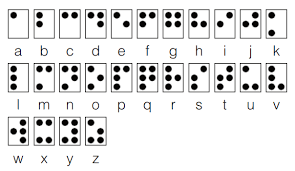
\includegraphics[width=1\textwidth]{Imagenes/Fuentes/SAAC/braille.png}
			\caption{Representaci�n del abecedario en el Sistema Braille}
			\label {fig: imgBraille}
		\end{figure}
		
		\item \textit{\textbf{Pictogramas:}} sistema que utiliza dibujos simples o s�mbolos para comunicarse de forma sencilla. Los s�mbolos son dise�ados con el fin de representar las palabras y conceptos de uso m�s com�n. Existen diversos sistemas pictogr�ficos, como por ejemplo MIC o ARASAAC, cuyos pictogramas son los m�s utilizados en Espa�a. En la Figura~\ref {fig: imgPictografico} se muestra la representaci�n de varios elementos comunes mediante pictogramas. 
		
		\begin{figure}[]
			\centering
			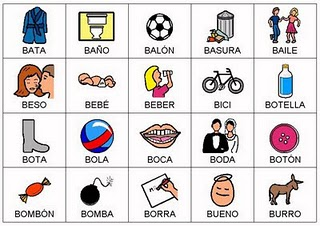
\includegraphics[width=0.9\textwidth]{Imagenes/Fuentes/SAAC/pictogramas.jpg}
			\caption{Representaci�n de distintas palabras con pictogramas}
			\label {fig: imgPictografico}
		\end{figure}
		
	\end{itemize}
\end{itemize}


%-------------------------------------------------------------------
\section{La Lengua de Signos}
%-------------------------------------------------------------------
\label{cap2:sec:La Lengua de Signos}

La Lengua de Signos (LS) \citep*{bkApuntesLing} es una lengua natural gestual que sirve para ayudar a integrarse a las personas con discapacidad auditiva o dificultad en el habla, y a personas que se quieran comunicar con ellas. La Lengua de Signos es considerada como SAAC gestual sin ayuda, es decir, no necesita apoyo de ning�n sistema de informaci�n (im�genes, pictogramas).\\ 

Esta lengua es rica y compleja gramaticalmente, es decir, no es una simple representaci�n literal de la lengua oral. Adem�s, es muy expresiva, ya que permite expresar sentimientos y emociones a la hora de comunicarse mediante el �nfasis en los gestos y expresiones faciales.\\

El desarrollo de esta lengua necesita de unas capacidades tanto cognitivas como motrices, as� como de un entrenamiento espec�fico. Este sistema puede tener una doble finalidad:

\begin{itemize}
	\item \textbf{Como elemento de comunicaci�n:} Para hacer posible la comunicaci�n de manera alternativa al habla o paliar las limitaciones que provoca la p�rdida auditiva y as� mejorar la integraci�n social de las personas que sufren esta discapacidad.
	
	
	
	\item \textbf{Como elemento de desarrollo intelectual:} la audici�n es el �rgano que m�s influye en la educaci�n, ya que es v�a de adquisici�n del lenguaje. El uso de estos sistemas es determinante en el desarrollo intelectual de las personas, sobre todo cuando el lenguaje verbal no est� adquirido.
	
\end{itemize}


La LS no es una lengua universal, es decir, no existe una Lengua de Signos com�n para todo el mundo ni para todos los idiomas. Cada pa�s puede contar con una o varias LS oficiales y no son �nicas para cada lengua. Esto quiere decir que dos pa�ses que comparten lengua oral oficial (como Espa�a y Argentina), tienen Lenguas de Signos totalmente diferentes. Incluso puede ocurrir que una misma LS presente diferencias dependiendo de en qu� regi�n del pa�s se utilice.\\

En Espa�a hay alrededor de 1.064.000 personas mayores de seis a�os con alg�n grado de discapacidad auditiva, de las cuales s�lo el 1,25\% (13.300 personas) utilizan la Lengua de Signos para comunicarse, seg�n los �ltimos datos aportados por el Instituto Nacional de Estad�stica (INE)\footnote{\url{https://www.ine.es/}}. Esto se debe  a que la mayor�a de las personas con esta discapacidad son capaces de comunicarse a trav�s del lenguaje oral, ya que su grado de discapacidad se lo permite y les ayuda a integrarse con el entorno debido a que no es com�n saber Lengua de Signos si no sufres de dicha discapacidad, siendo �nicamente alrededor de 400.000 las personas que saben comunicarse mediante dicha lengua en nuestro pa�s. Desde el a�o 2007 Espa�a cuenta con dos LS oficiales: la Lengua de Signos Espa�ola (LSE) y la Lengua de Signos Catalana (LSC), siendo la LSE la m�s utilizada en nuestro pa�s.\\


La LSE es una lengua normativizada, es decir, consta de unas reglas que marcan el correcto uso de la misma.

%-------------------------------------------------------------------
\subsection{Reglas de la Lengua de Signos Espa�ola}
%-------------------------------------------------------------------
A continuaci�n, se explica el conocimiento b�sico de estas normas en lo referente a la gram�tica, fonolog�a, sintaxis y morfolog�a.

%-------------------------------------------------------------------
\subsubsection{Fonolog�a de la Lengua de Signos Espa�ola}
%-------------------------------------------------------------------

La fonolog�a  \citep*{bkApuntesLing}, en lo relativo a la LSE,  se refiere al estudio de la estructura y organizaci�n interna de los signos.\\

Los signos de la LSE est�n formados por siete elementos esenciales:

\begin{itemize}
	\item \textbf{Forma o configuraci�n de la mano o manos} que intervienen en el signo. Es importante remarcar que no se utilizan los t�rminos ``mano izquierda'' y ``mano derecha'', ya que dependiendo de la persona, la mano dominante puede ser una u otra. Por eso se utilizan los t�rminos ``mano dominante'' y ``mano no dominante'' para se�alar con qu� mano o manos signar. Para indicar qu� mano es la dominante basta con levantarla y rotarla (tal y como se muestra en la Figura~\ref {fig: imgLSEConfig})
	
	\begin{figure}[]
		\centering
		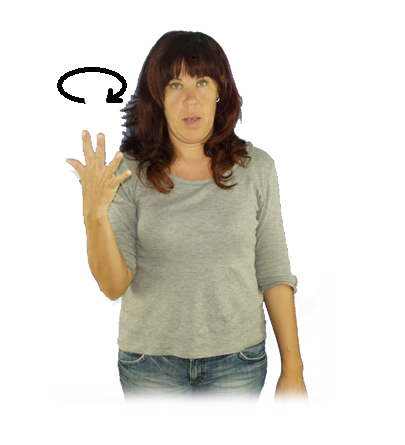
\includegraphics[width=0.5\textwidth]{Imagenes/Fuentes/SAAC/LSEConfig.png}
		\caption{Representaci�n de la configuraci�n de la mano en Lengua de Signos }
		\label {fig: imgLSEConfig}
	\end{figure}
	
	\item \textbf{Orientaci�n} de la mano o manos al signar respecto al cuerpo del individuo. Por ejemplo, gestos como \textit{``ayudar''}, el cual podemos observar en la Figura~\ref {fig: imgLSEAyudar}, van acompa�ados de direcci�n para indicar a qu� persona se refiere el emisor. En la Figura~\ref {fig: imgLSEOrient} se muestran las distintas direcciones que pueden acompa�ar a los gestos. 
	
	\begin{figure}[]
		\centering
		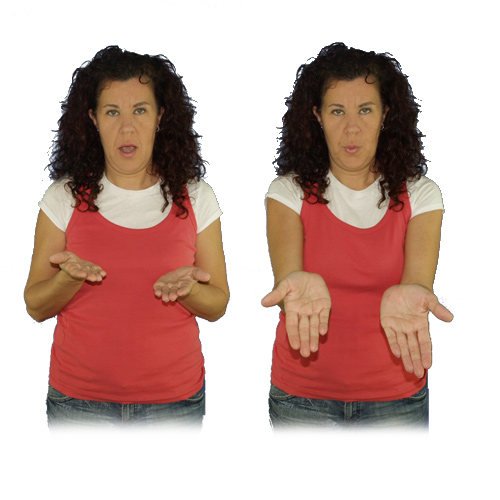
\includegraphics[width=0.45\textwidth]{Imagenes/Fuentes/SAAC/LSEAyudar.jpg}
		\caption{Signo \textit{``ayudar''} en LSE del banco de im�genes ARASAAC}
		\label {fig: imgLSEAyudar}
	\end{figure}
	
	\begin{figure}[]
		\centering
		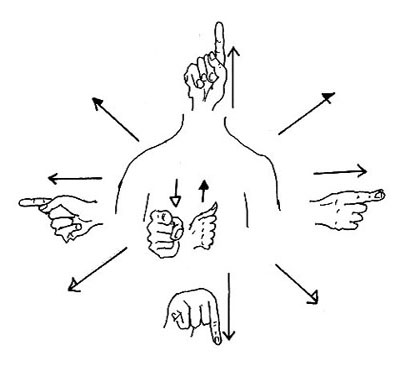
\includegraphics[width=0.5\textwidth]{Imagenes/Fuentes/SAAC/LSEOrient.jpg}
		\caption{Representaci�n de la orientaci�n de las manos en Lengua de Signos }
		\label {fig: imgLSEOrient}
	\end{figure}
	
	
	\item \textbf{Lugar de articulaci�n} del signo, es decir, el espacio en el que se realiza el movimiento. Puede ser ante el pecho, el hombro, la frente o los labios, entre otros. Por ejemplo, en la Figura~\ref {fig: imgLSEVisera}, el gesto referente a la palabra ``visera'' se realiza ante la frente.
	\item \textbf{Plano} en el que se realiza el signo, es decir, la distancia de realizaci�n del signo con respecto al cuerpo del individuo. Sirve para indicar el tiempo verbal de los gestos. Los gestos signados m�s cerca del cuerpo indican pasado y lo m�s alejados futuro.
	\item \textbf{Punto de contacto} de la mano dominante con el cuerpo del individuo al realizar el signo. Por ejemplo, al signar \textit{``oir''} el punto de contacto ser�a la oreja, tal y como se muestra en la Figura~\ref {fig: imgLSEPntContc}.
	
	\begin{figure}[]
		\centering
		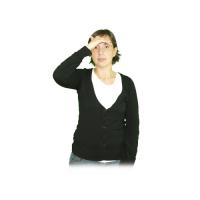
\includegraphics[width=0.5\textwidth]{Imagenes/Fuentes/SAAC/LSEVisera.jpg}
		\caption{Signo \textit{``visera''} en LSE del banco de im�genes ARASAAC }
		\label {fig: imgLSEVisera}
	\end{figure}
	
	\begin{figure}[]
		\centering
		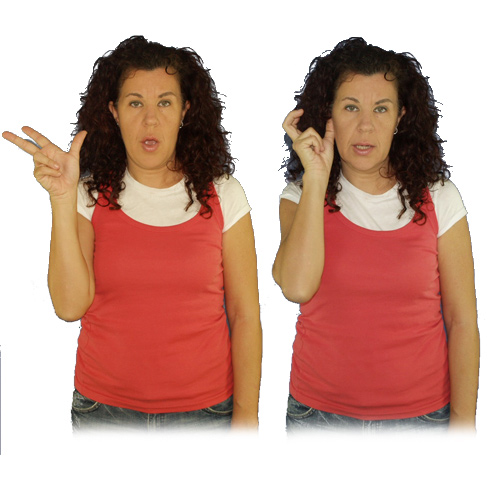
\includegraphics[width=0.5\textwidth]{Imagenes/Fuentes/SAAC/LSEPntContc.jpg}
		\caption{Signo \textit{``oir''} en LSE del banco de im�genes ARASAAC }
		\label {fig: imgLSEPntContc}
	\end{figure}
	
	
	\item \textbf{Movimiento} de las manos al realizar un signo. Puede ser giratorio, vaiv�n o quebrado, entre otros. Podemos observar en que consisten algunos de estos movimientos en la Figura~\ref {fig: imgLSEMovimientos}
	\item \textbf{Componente no manual} del signo, que puede ser desde expresiones faciales hasta movimientos corporales del individuo. Por ejemplo, en la Figura~\ref {fig: imgLSEMucho}, la int�rprete quiere expresar una cantidad abundante, acompa�ando al signo de una expresi�n facial que enfatiza una gran cantidad.
	
	\begin{figure}[]
		\centering
		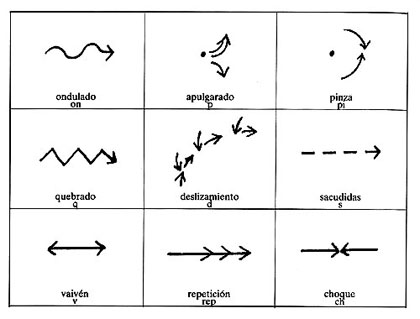
\includegraphics[width=1\textwidth]{Imagenes/Fuentes/SAAC/LSEMovimientos.jpg}
		\caption{Ejemplos de tipos de movimientos realizados al signar en LSE }
		\label {fig: imgLSEMovimientos}
	\end{figure}
	
	\begin{figure}[]
		\centering
		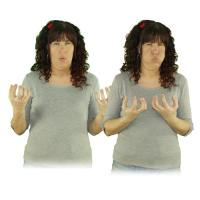
\includegraphics[width=0.5\textwidth]{Imagenes/Fuentes/SAAC/LSEMucho.jpg}
		\caption{Signo \textit{``mucho''} en LSE del banco de im�genes ARASAAC }
		\label {fig: imgLSEMucho}
	\end{figure}
\end{itemize}


%-------------------------------------------------------------------
\subsubsection{Sintaxis de la Lengua de Signos Espa�ola}
%-------------------------------------------------------------------

Las oraciones en la LSE no se estructuran igual que en castellano. La LSE es una lengua anal�tica, es decir, la estructura de las oraciones es muy simple, tendiendo a simplificar las frases para comunicar la informaci�n de la manera m�s concisa posible, al igual que lenguas como japon�s o alem�n.\\

La estructura b�sica de las oraciones se compone de sujeto-objeto-verbo, aunque existen excepciones. Por ejemplo, la oraci�n \textit{``�l come patatas''} en LSE se traducir�a como \textit{``�l patatas comer''}. Seg�n se van incorporando elementos a las oraciones, la estructura se va volviendo m�s compleja siguiendo un orden temporal, es decir, las acciones se nombran en el orden en el que suceden. Por ejemplo, la oraci�n \textit{``Despu�s de comer me fui a dormir''}, se traducir�a a LSE como \textit{``Yo comer fin dormir ir''}, indicando que primero se realiz� la acci�n de comer y despu�s la acci�n de irse a dormir.


%-------------------------------------------------------------------
\subsubsection{Morfolog�a de la Lengua de Signos Espa�ola}
%-------------------------------------------------------------------

En la lengua oral, los morfemas de g�nero sirven principalmente para marcar la concordancia entre el sustantivo y el adjetivo. En la LSE esto no existe, ya que tanto los adjetivos como los sustantivos son palabras invariables y adem�s, no existen los art�culos. Los elementos inanimados no tienen g�nero en la LSE, por lo que no es necesario signarlos, mientras que los elementos animados s� que precisan de distinci�n. En caso de que se quiera hacer �nfasis en el g�nero de alguna palabra, al terminar de signar la palabra en cuesti�n se a�aden los signos de  \textit{``hombre''} (Figura~\ref {fig: imgLSEHombre}) o de  \textit{``mujer''} (Figura~\ref {fig: imgLSEMujer}).\\


\begin{figure}[]
	\centering
	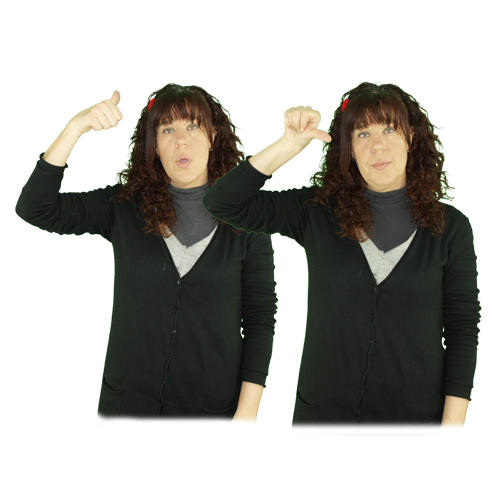
\includegraphics[width=0.45\textwidth]{Imagenes/Fuentes/SAAC/LSEHombre.jpg}
	\caption{Signo \textit{``hombre''} del banco de im�genes ARASAAC }
	\label {fig: imgLSEHombre}
\end{figure}

\begin{figure}[]
	\centering
	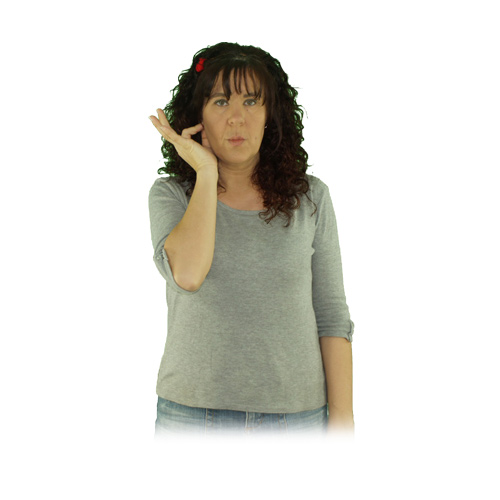
\includegraphics[width=0.4\textwidth]{Imagenes/Fuentes/SAAC/LSEMujer.jpg}
	\caption{Signo \textit{``mujer''} del banco de im�genes ARASAAC }
	\label {fig: imgLSEMujer}
\end{figure}

En las Figuras~\ref {fig: imgLSEAbuelo} y~\ref {fig: imgLSEAbuela} podemos observar c�mo se a�aden los signos \textit{``hombre''} y \textit{``mujer''} para marcar el g�nero de las palabras \textit{``abuela''} y \textit{``abuelo''}.\\

\begin{figure}[]
	\centering
	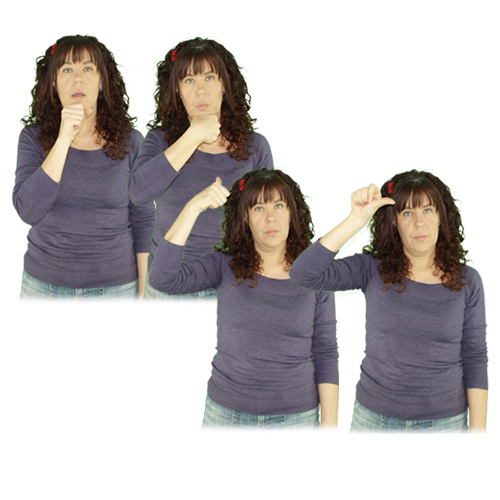
\includegraphics[width=0.45\textwidth]{Imagenes/Fuentes/SAAC/LSEAbuelo.jpg}
	\caption{Signo \textit{``abuelo''} del banco de im�genes ARASAAC }
	\label {fig: imgLSEAbuelo}
\end{figure}

\begin{figure}[]
	\centering
	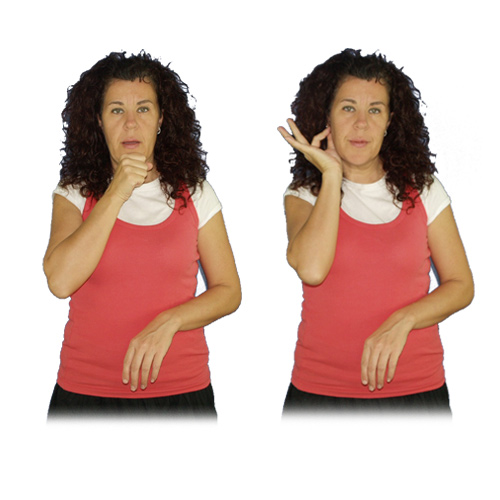
\includegraphics[width=0.4\textwidth]{Imagenes/Fuentes/SAAC/LSEAbuela.jpg}
	\caption{Signo \textit{``abuela''} del banco de im�genes ARASAAC }
	\label {fig: imgLSEAbuela}
\end{figure}


Existen algunas excepciones, como el caso de los signos para \textit{``ni�o''} y \textit{``ni�a''}, los cuales tienen su propio signo para definir el g�nero de la palabra. Podemos verlos en la Figura~\ref {fig: imgLSENi�o} y en la Figura~\ref {fig: imgLSENi�a} respectivamente.\\


\begin{figure}[]
	\centering
	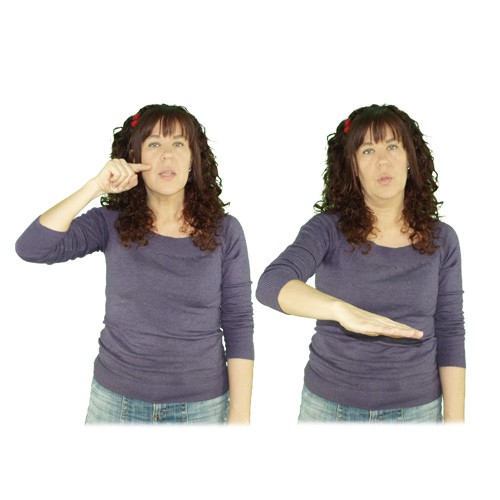
\includegraphics[width=0.45\textwidth]{Imagenes/Fuentes/SAAC/LSENino.jpg}
	\caption{Signo \textit{``ni�o''} del banco de im�genes ARASAAC }
	\label {fig: imgLSENi�o}
\end{figure}

\begin{figure}[]
	\centering
	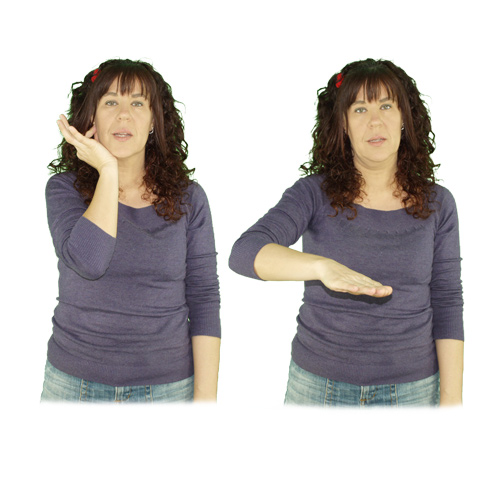
\includegraphics[width=0.45\textwidth]{Imagenes/Fuentes/SAAC/LSENina.jpg}
	\caption{Signo \textit{``ni�a''} del banco de im�genes ARASAAC }
	\label {fig: imgLSENi�a}
\end{figure}

Por otra parte, los morfemas de n�mero en la LSE sirven �nicamente para expresar cantidad. Existen varias formas de expresar cantidad seg�n la categor�a gramatical de la palabra a la que acompa�en:


\begin{itemize}
	
	\item \textbf{Sustantivos: }
	\begin{itemize}
		\item Si no queremos enfatizar el n�mero o queremos expresar solo una unidad, se signa la palabra sin a�adir nada a ella. Por ejemplo, la frase \textit{``La puerta de la universidad es de color gris''} en LSE ser�a \textit{``Universidad puerta color gris''}.\\
		
		\item Se pueden a�adir palabras que expresen cantidad, como cuantificadores definidos, por ejemplo \textit{``uno''}, cuyo signo podemos observar en la Figura~\ref {fig: imgLSEUno}, o cuantificadores indefinidos, por ejemplo \textit{``muchos''}, cuyo signo podemos observar en la Figura~\ref {fig: imgLSEMuchos}.\\
		
		\item Se puede enfatizar la cantidad de un sustantivo mediante la expresi�n facial de la cual se puede distinguir si es mucha o poca la cantidad a la que se quiere referir el emisor. Por ejemplo, en la Figura~\ref {fig: imgLSEMuchos} aparece una int�rprete realizando el signo \textit{``muchos''}. En ella podemos observar el gesto facial indicando una gran cantidad. Esta gesticulaci�n puede sustituir al propio signo \textit{``muchos''} en una oraci�n si se realiza mientras se signa la oraci�n.
		
	\end{itemize}
	
	
	\begin{figure}[]
		\centering
		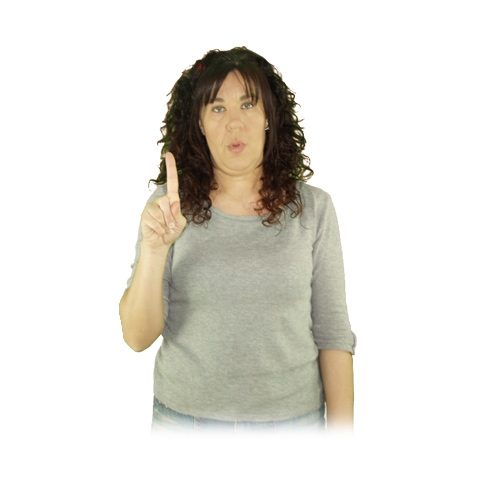
\includegraphics[width=0.45\textwidth]{Imagenes/Fuentes/SAAC/LSEUno.jpg}
		\caption{Signo \textit{``uno''} del banco de im�genes ARASAAC }
		\label {fig: imgLSEUno}
	\end{figure}
	
	\begin{figure}[]
		\centering
		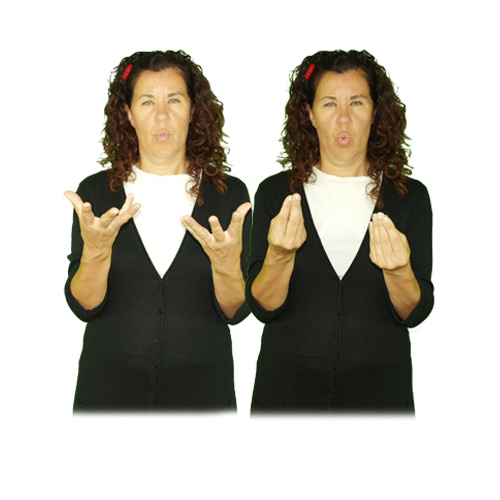
\includegraphics[width=0.45\textwidth]{Imagenes/Fuentes/SAAC/LSEMuchos.jpg}
		\caption{Signo \textit{``muchos''} del banco de im�genes ARASAAC }
		\label {fig: imgLSEMuchos}
	\end{figure}
	
	
	\item \textbf{Adjetivos:} no var�an en cuanto a n�mero.
	\item \textbf{Verbos:} el plural se realiza principalmente mediante la repetici�n del verbo y recae sobre el objeto. Por ejemplo, en la oraci�n \textit{``Yo viajo a muchos sitios''} se repetir�a el verbo viajar: \textit{``Yo viajar viajar sitio''}. \\
	
\end{itemize}

%-------------------------------------------------------------------
\subsubsection{Verbos de la Lengua de Signos Espa�ola}
%-------------------------------------------------------------------
El verbo en la LSE \citep*{tchVerbos} presenta unos rasgos gramaticales propios que es necesario tener en cuenta. Se distinguen tres clases b�sicas de verbos en LSE:

\begin{itemize}
	\item \textbf{Verbos planos:} Los verbos planos son aquellos cuyo signo no se modifica para marcar informaci�n complementaria, como por ejemplo el g�nero, el n�mero o a qui�n va dirigida la acci�n. Para a�adir este tipo de informaci�n se a�aden palabras independientes, como cuantificadores (uno, dos, etc), pronombres personales (yo, �l, etc). Por ejemplo, \textit{Querer, Comer, Pensar, Conducir, etc.} Podemos observar en la Figura~\ref {fig: imgLSEQuerer} como el signo de la palabra \textit{``Querer''} no aporta ning�n tipo de informaci�n adicional por s� mismo. 
	
	\item \textbf{Verbos de concordancia:} Los verbos de concordancia son aquellos que en la realizaci�n del propio signo se a�ade informaci�n adicional, como por ejemplo, a qui�n va dirigida la acci�n mediante la articulaci�n del signo. Esto podemos observarlo en la Figura~\ref {fig: imgLSEAyudar}, que muestra el signo de la palabra \textit{``ayudar''}, el cual termina se�alando en el espacio a la persona a la que se est� ayudando. Algunos ejemplos de verbos de concordacia son: \textit{Avisar, Ayudar, Contar, Cuidar, Responder, etc.} 
	
	
	\item \textbf{Verbos espaciales:} Los verbos espaciales son aquellos que no necesitan un signo espec�fico para expresar su significado, ya que indican la situaci�n en el espacio de algo o alguien a trav�s de la direcci�n y la velocidad con la que se realiza el signo. Al igual que en los verbos planos, se puede a�adir informaci�n adicional como g�nero o n�mero a trav�s de palabras independientes, como cuantificadores. Por ejemplo, \textit{``Hay un rat�n ah�''} se traduce como \textit{``Rat�n (Se�alando el sitio)''}. Esto podemos observarlo en la Figura~\ref {fig: imgLSESe�alar}, en la que se muestra el signo de la palabra \textit{``se�alar''}. 
	
	\begin{figure}[]
		\centering
		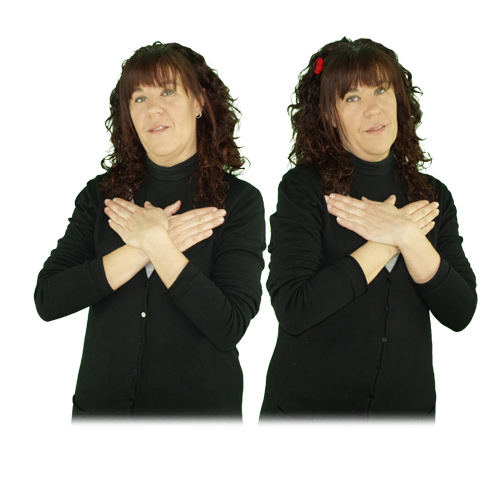
\includegraphics[width=0.45\textwidth]{Imagenes/Fuentes/SAAC/LSEQuerer.jpg}
		\caption{Signo \textit{``querer''} en LSE del banco de im�genes ARASAAC}
		\label {fig: imgLSEQuerer}
	\end{figure}
	
	
	
	\begin{figure}[]
		\centering
		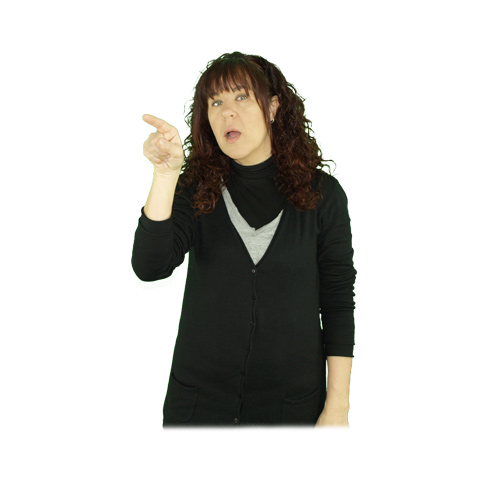
\includegraphics[width=0.45\textwidth]{Imagenes/Fuentes/SAAC/LSESenalar.jpg}
		\caption{Signo \textit{``se�alar''} en LSE del banco de im�genes ARASAAC}
		\label {fig: imgLSESe�alar}
	\end{figure}
	
\end{itemize} 


%-------------------------------------------------------------------
\subsection{Bancos de videos e im�genes LSE}
%-------------------------------------------------------------------

%-------------------------------------------------------------------
\subsubsection{ARASAAC}
%-------------------------------------------------------------------

El Portal Aragon�s de la Comunicaci�n Aumentativa y Alternativa (ARASAAC)\footnote {\url{http://www.arasaac.org/}}, es un proyecto desarrollado en el a�o 2007 por el gobierno de Arag�n. Tiene como objetivo la creaci�n de un sistema pictogr�fico de comunicaci�n y un conjunto de herramientas de libre distribuci�n. Estos recursos facilitan la accesibilidad de car�cter comunicativo y cognitivo en diversos �mbitos de la vida a todas las personas que lo puedan requerir. ARASAAC proporciona un cat�logo con m�s de 8.000 pictogramas en color, en blanco y negro, fotograf�as, as� como un banco de v�deos e im�genes a color de signos de la Lengua de Signos Espa�ola. En la Figura~\ref {fig: imgLSEHola} se muestra el signo \textit{``hola''} en LSE del banco de im�genes de LSE de ARASAAC. Este contenido est� disponible como contenido descargable con licencia Creative Commons, es decir, se puede usar libremente sin �nimo de lucro. \\

ARASAAC ofrece una API\footnote {\url{https://beta.arasaac.org/developers/api}} a trav�s de la cual se pueden obtener sus pictogramas y los materiales generados con sus pictogramas a trav�s de llamadas a los m�todos de dicha API. Para obtener los recursos correspondientes a la LSE es necesario descargarlos a trav�s del apartado de descargas de su p�gina web\footnote {\url{http://www.arasaac.org/descargas.php}}.


\begin{figure}[]
	\centering
	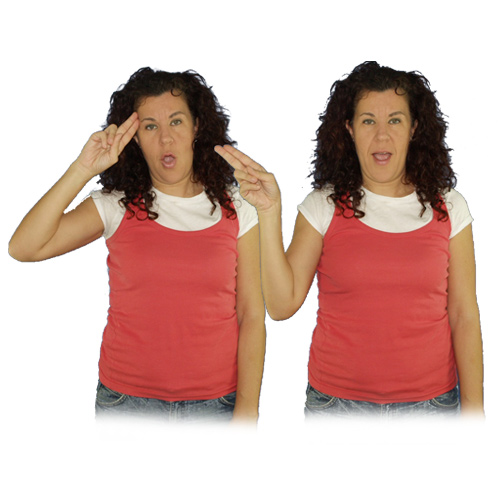
\includegraphics[width=0.45\textwidth]{Imagenes/Fuentes/SAAC/LSEHola.jpg}
	\caption{Signo \textit{``hola''} en LSE del banco de im�genes ARASAAC}
	\label {fig: imgLSEHola}
\end{figure}




%-------------------------------------------------------------------
\subsubsection{Banco de im�genes Fundacion CNSE}
%-------------------------------------------------------------------
La Confederaci�n Estatal de Personas Sordas (CNSE)\footnote{\url{http://www.fundacioncnse.org/}}  es una organizaci�n que  atiende los intereses de las personas sordas y sus familias en Espa�a. Es la primera entidad asociativa de la  discapacidad de nuestro pa�s, y desde su creaci�n se ha ocupado de incentivar el desarrollo y la participaci�n social de dicho colectivo. En ella se integran 17 federaciones de personas sordas, una por cada comunidad aut�noma, que, a su vez, mantienen afiliadas a m�s de 120 asociaciones provinciales y locales de todo el Estado. No obstante, la CNSE atiende cualquier necesidad relacionada con el colectivo de personas sordas, est�n o no afiliadas a su movimiento asociativo.\\

En 1998, la CNSE constituye la Fundaci�n CNSE para la Supresi�n de las Barreras de Comunicaci�n. Se trata de una organizaci�n estatal sin �nimo de lucro, desde la que se impulsa la investigaci�n y el estudio de la Lengua de Signos Espa�ola y se trabaja por mejorar la accesibilidad de las personas sordas en todos los �mbitos y se promueve el desarrollo de proyectos que mejoren la calidad de vida de las personas sordas y de sus familias.\\

Esta fundaci�n cuenta con un banco de im�genes\footnote{\url{http://www.fundacioncnse.org/educa/bancolse/}} (ver Figura~\ref {fig: imgFundCNSE}) y signos de la LSE, accesible a trav�s de su p�gina web. En esta p�gina no existe la opci�n de descargar todas las im�genes de una vez, sino que es necesario hacerlo manualmente una a una, y no cuenta con un banco de videos de signos.\\


\begin{figure}[]
	\centering
	\includegraphics[width=1\textwidth]{Imagenes/Fuentes/Apps/fundCNSE.png}
	\caption{Recursos LSE de la Fundaci�n CNSE}
	\label {fig: imgFundCNSE}
\end{figure}

%-------------------------------------------------------------------
\subsubsection{SpreadTheSign}
%-------------------------------------------------------------------
SpreadTheSign\footnote{\url{https://www.spreadthesign.com/es.es/search/}} es un diccionario online administrado por el Centro Europeo de Lenguas de Signos, que cuenta con m�s de 400.000 signos en v�deo (ver Figura~\ref {fig: imgSpreadTheSign}) de diferentes Lenguas de Signos, como la espa�ola, estadounidense o alemana, entre muchas otras, as� como de un alfabeto dactilol�gico para cada una de ellas y frases previamente almacenadas. Es una herramienta de autoaprendizaje gratuita, accesible a trav�s de su p�gina web y desde su aplicaci�n para Android\footnote{\url{https://play.google.com/store/apps/details?id=com.spreadthesign.androidapp_paid&hl=es}} e IOS\footnote{\url{https://apps.apple.com/ni/app/spreadthesign/id438811366}}, aunque ninguna de estas aplicaciones permite la descarga de contenido. 


\begin{figure}[]
	\centering
	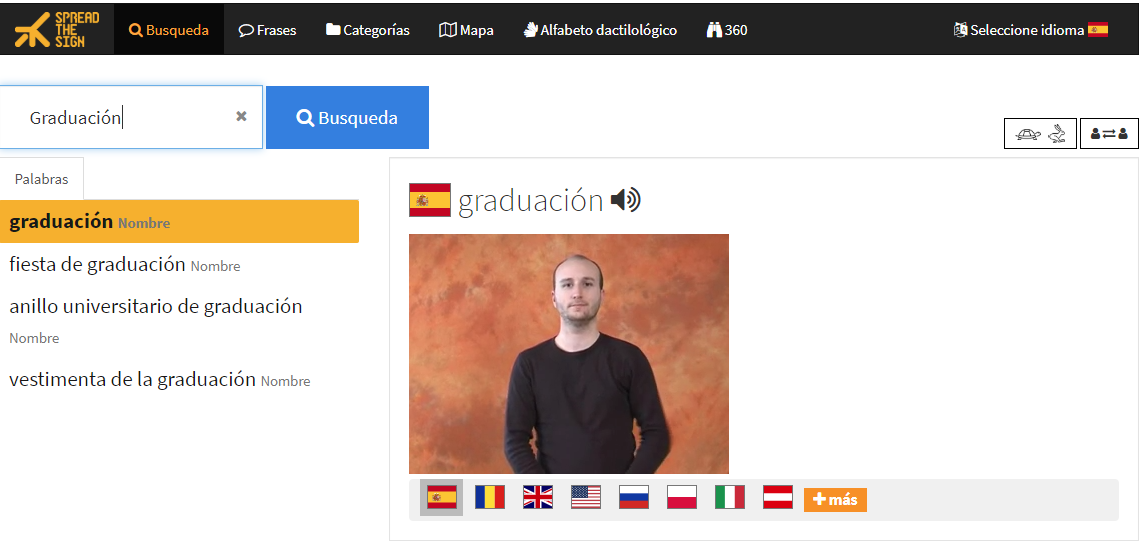
\includegraphics[width=1\textwidth]{Imagenes/Fuentes/Apps/SpreadTheSign_1.png}
	\caption{Imagen de la p�gina web SpreadTheSign}
	\label {fig: imgSpreadTheSign}
\end{figure}


%-------------------------------------------------------------------
\section{Aplicaciones de Traducci�n de Texto a LSE}
%-------------------------------------------------------------------
La variedad de recursos y aplicaciones orientadas a la integraci�n social de las personas con discapacidad auditiva ha ido aumentado con el paso del tiempo. En esta secci�n se presentan aplicaciones con un objetivo similar al de nuestro TFG cuyo prop�sito es ayudar en la integraci�n de las personas que sufren de discapacidad auditiva.


%-------------------------------------------------------------------
\subsection{Text2Sign}
\label{Text2Sign}
%-------------------------------------------------------------------
Text2Sign\footnote{\url{http://text2sign.es/}} es una aplicaci�n tanto web como m�vil gratuita que permite enviar un texto en formato PDF, imagen o Word a un equipo de int�rpretes que se encarga de traducirlo a la LSE. Una vez realizada la traducci�n se puede descargar a trav�s de la plataforma entre un periodo de 24 y 72 horas dependiendo de la longitud del texto ya que no es un servicio instant�neo y est� limitado a una o dos p�ginas.


%-------------------------------------------------------------------
\subsection{TextoSign}
%-------------------------------------------------------------------

TextoSign\footnote{\url{http://textosign.es/}} es una herramienta software que funciona en p�ginas web, asistentes virtuales y dispositivos m�viles que traduce en tiempo real un texto a la Lengua de Signos Espa�ola mediante un int�rprete visual llamado Maya (Figura~\ref {fig: imgTextSign}). Se trata de herramienta de pago y es utilizada hoy en d�a por La Caixa, Adif, Inturjoven y otras entidades.

\begin{figure}[]
	\centering
	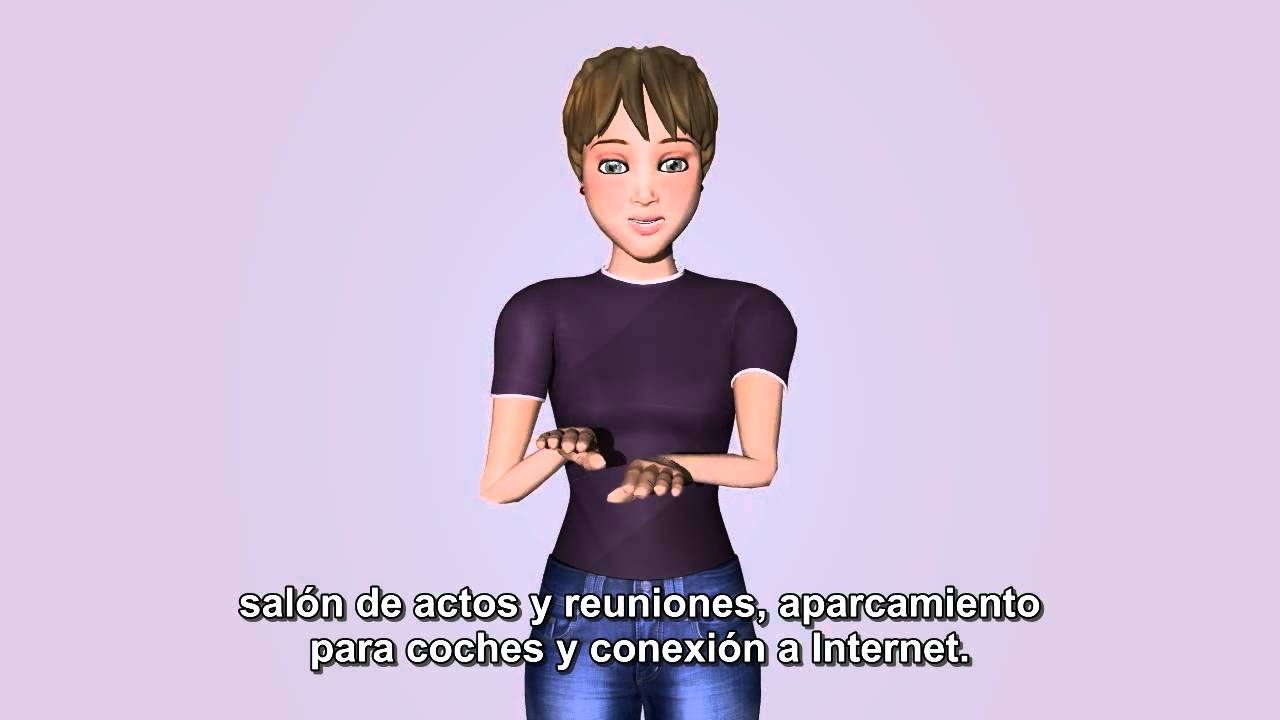
\includegraphics[width=0.8\textwidth]{Imagenes/Fuentes/Apps/textsign.jpg}
	\caption{Maya, avatar usado por TextoSign.}
	\label {fig: imgTextSign}
\end{figure}


%-------------------------------------------------------------------
\subsection{StorySign}
%-------------------------------------------------------------------
StorySign\footnote{\url{https://play.google.com/}} es una aplicaci�n para Android gratuita desarrollada por Huawei, que traduce en tiempo real  una selecci�n de cuentos infantiles a diferentes Lenguas de Signos como la espa�ola, italiana, francesa o inglesa. Para utilizarla es necesario abrir la aplicaci�n y sostener el m�vil encima del libro f�sico (especialmente dise�ado para esta aplicaci�n). Un avatar llamado Star interpreta el cuento en Lengua de Signos mientras la aplicaci�n resalta cada palabra que Star interpreta como podemos ver en la Figura~\ref {fig: imgStorySign}.

\begin{figure}[]
	\centering
	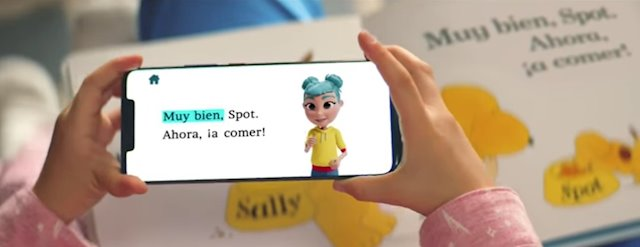
\includegraphics[width=1\textwidth]{Imagenes/Fuentes/Apps/storySign_1.jpg}
	\caption{Imagen de la aplicaci�n StorySign.}
	\label {fig: imgStorySign}
\end{figure}

%-------------------------------------------------------------------
\subsection{TeCuento}
%-------------------------------------------------------------------
TeCuento\footnote{\url{https://play.google.com/}}  es una aplicaci�n Android gratuita que contiene diversos cuentos que se reproducen en video con subt�tulos y LSE, como podemos apreciar en la Figura~\ref {fig: imgTeCuento}. No se traduce en el momento, son videos previamente grabados por personas f�sicas dando tambi�n la opci�n de poder escribir tu propio cuento y que lo traduzcan a LSE.



\begin{figure}[]
	\centering
	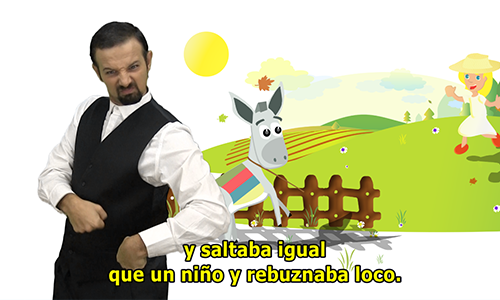
\includegraphics[width=1\textwidth]{Imagenes/Fuentes/Apps/teCuento_1.png}
	\caption{Imagen de la aplicaci�n TeCuento.}
	\label {fig: imgTeCuento}
\end{figure}

%-------------------------------------------------------------------
\subsection{Conclusiones}
%-------------------------------------------------------------------


Como se ha podido comprobar existe un abanico amplio de aplicaciones que son capaces de traducir texto a LSE. Estas herramientas en su mayor�a cumplen el prop�sito de facilitar el uso de la Lengua de Signos a las personas que quieran comunicarse con ella. No obstante, presentan algunas limitaciones como licencias de pago, tiempo de respuesta lento o disponibilidad en un solo tipo de dispositivo.\\

Nuestro proyecto Text2LSE pretende solventar muchas de estas limitaciones proporcionando una aplicaci�n gratuita que sea accesible desde cualquier dispositivo, ya sea web o m�vil. El objetivo es ofrecer una traducci�n al instante de cualquier frase o palabra en castellano a LSE y la posibilidad de integrarse mediante servicios web en aplicaciones que requieran su uso.























%---------------------------------------------------------------------
%
%                          Cap�tulo 3
%
%---------------------------------------------------------------------

\chapter{Herramientas utilizadas}

\begin{FraseCelebre}
	\begin{Frase}
		"Controlar la complejidad es la esencia de la programaci�n". 
	\end{Frase}
	\begin{Fuente}
		Brian Kernigan
	\end{Fuente}
\end{FraseCelebre}


Introducci�n capitulo 3 COMPLETAR 
\\



%-------------------------------------------------------------------
\section{Python}
%-------------------------------------------------------------------
\label{cap3:sec:Python}

Python \citep*{tchDesarrolloWeb} es un lenguaje de programaci�n desarrollado a lo largo de la d�cada de los a�os 80 por Guido Vam Rossum. El objetivo del creador era desarrollar un lenguaje de programaci�n orientado a objetos de uso sencillo que sirviese para programar diversos tipos de tareas, no limitarlo a un solo tipo de uso. Sus principales caracter�sticas son:

\begin{itemize}
	
	\item \textbf{Din�mico:} Se puede utilizar para desarrollar desde simples scripts o p�ginas web hasta para servidores de gran potencia.
	
	\item \textbf{Interpretado:} El programador no necesita realizar el paso de compilar el c�digo, ya que Python se encarga de hacer esa compilaci�n por s� mismo de manera que el desarrollador  no tiene que realizar ese paso extra.
	
	\item \textbf{Multiplataforma:} Se puede utilizar en cualquier sistema inform�tico, siempre y cuando se haya instalado previamente un int�rprete compatible con �l.
	
	\item \textbf{Interactivo:} Python contiene un int�rprete por l�nea de comandos, a trav�s del cual se pueden introducir sentencias y ver en tiempo real el resultado de dicha sentencia.
	
	\item \textbf{Orientado a objetos:} el c�digo se estructura en elementos llamados clases, a trav�s de las cuales se crean los objetos con funcionalidades espec�ficas.
	
	\item \textbf{Funciones y librer�as:} python incluye una serie de funciones incluidas de base, como por ejemplo, la manipulaci�n de strings, n�meros, etc. A parte, existen multitud de librer�as que se pueden importar al desarrollar un programa para cubrir necesidades espec�ficas, como por ejemplo, el procesamiento del lenguaje natural.
	
	\item \textbf{Sintaxis clara:} La estructura del c�digo se basa en los m�rgenes de obligado cumplimiento, siendo as� muy visual. Esto hace que sea m�s sencillo distinguir las distintas partes del c�digo.
	
	\item \textbf{Licencia de c�digo abierto} \citep*{tchPython}: Licencia compatible con la Licencia p�blica general de GNU, la cual permite que el usuario final pueda tener acceso al c�digo, descargarlo, copiarlo y manipularlo.
	
\end{itemize}

Se ha decidido utilizar Python en este proyecto debido a la facilidad de uso y a la existencia de diversas librer�as de procesamiento de lenguaje natural, como Spacy y NLTK, las cuales se describen en los apartados previos \hyperref[cap2:sec:PLN:subsec:Spacy]{``Spacy''} y \hyperref[cap2:sec:PLN:subsec:NLTK]{``NLTK''} respectivamente.



%-------------------------------------------------------------------
\section{Flask}
%-------------------------------------------------------------------
\label{cap2:sec:Flask}
Flask es un ``micro'' Framework escrito en Python y concebido para facilitar el desarrollo de Aplicaciones Web y APIs.\\

La palabra micro hace referencia a que Flask �nicamente trae por defecto las herramientas necesarias para crear una aplicaci�n web b�sica, aunque si se necesitan a�adir nuevas funcionalidades hay un conjunto muy grande de extensiones (plugins) que se pueden instalar f�cilmente. Por ello, Flask es muy recomendable para el desarrollo de aplicaciones que no requieran muchas extensiones o que se necesiten implementar de una forma �gil y r�pida. Tambi�n es muy recomendable para implementar microservicios.\\

Algunas de las caracter�sticas de Flask por las que decidimos desarrollar nuestra API con este framework son las siguientes:\\

\newpage
\begin{itemize}
	
	\item Rapidez y facilidad en la instalaci�n y configuraci�n, a diferencia de otros frameworks como Django, que tiene una curva de aprendizaje mucho m�s baja.
	
	\item Es compatible con Python. Nuestra API est� implementada en dicho lenguaje.
	
	\item Incluye un servidor web de desarrollo. No se necesita una infraestructura con un servidor web para probar las aplicaciones, sino que de una manera sencilla se puede levantar un servidor web para ir viendo los resultados que se van obteniendo.
	
	\item Cuenta con depurador. Si tenemos alg�n error en el c�digo que se est� desarrollando, se puede depurar ese error y ver los valores de las variables.
	
	\item Flask es Open Source y est� amparado bajo una licencia BSD, que es la licencia utilizada para los sistemas operativos BSD (Berkeley Software Distribution), y tiene menos restricciones en comparaci�n con otras licencias como la GPL, estando muy cercana al dominio p�blico.
	
	\item Cuenta con una muy buena documentaci�n.
	
\end{itemize}


%-------------------------------------------------------------------
\section{Nginx}
%-------------------------------------------------------------------
\label{cap2:sec:Nginx}

Nginx \footnote{Web oficial de Nginx \url{https://www.nginx.com/}} es un servidor web de alto rendimiento, capaz de trabajar junto con diversas tecnolog�as de desarrollo y lenguajes. La asincron�a es una de sus caracter�sticas fundamentales, junto con su rapidez, debido a que es un servidor web ligero.
A d�a de hoy, adem�s de sus capacidades de servidor HTTP, NGINX tambi�n puede funcionar como un servidor proxy para correo electr�nico (IMAP, POP3 y SMTP) y un proxy inverso y equilibrador de carga para servidores (HTTP, TCP y UDP).\\

Las ventajas de NGINX y el porqu� de su uso:

\begin{itemize}
	
	\item Nginx es un software multiplataforma que se puede usar en la gran mayor�a de los sistemas operativos, tanto en sistemas basados en Unix como en Windows.
	
	\item Consume menos recursos que la mayor�a de servicios que hacen su misma funci�n ya que hace un uso de memoria de forma est�tica y se mantiene bastante estable independientemente del volumen de tr�fico.
	
	\item Proporciona un alto rendimiento sobre todo en casos de mucho tr�fico.
	
	\item Puede ser usado como Proxy inverso cacheando el contenido de nuestros sitios web.
	
	
\end{itemize}















%---------------------------------------------------------------------
%
%                          Cap�tulo 4
%
%---------------------------------------------------------------------

\chapter{Metodolog�as utilizadas}

\begin{FraseCelebre}
	\begin{Frase}
		"Juntarse es un comienzo. Seguir juntos es un progreso. Trabajar juntos es un �xito". 
	\end{Frase}
	\begin{Fuente}
		Henry Ford
	\end{Fuente}
\end{FraseCelebre}

En este cap�tulo se habla de la metodolog�a de trabajo seguida por el equipo de este TFG durante el desarrollo del mismo, junto con algunas de las herramientas utilizadas para organizar y estructurar las tareas a realizar por cada uno de los miembros y mantener el c�digo de la aplicaci�n accesible y con sus correspondientes copias de seguridad. COMPLETAR

%-------------------------------------------------------------------
\section{Metodolog�as �giles}
%-------------------------------------------------------------------
\label{cap4:sec:Metodologias Agiles}

Las metodolog�as �giles \citep*{tchMetAgiles} son aquellas que permiten adaptar la forma de trabajo a las condiciones particulares de cada proyecto, consiguiendo flexibilidad e inmediatez en la respuesta para amoldar el proyecto y su desarrollo a las circunstancias espec�ficas del entorno.\\


La aplicaci�n de metodolog�as �giles permite involucrar a nuestros tutores a lo largo de todo el proyecto. En cada etapa se informa de los logros y progresos del mismo, con la visi�n de involucrarles directamente para sumar su experiencia y conocimiento, y as� optimizar las caracter�sticas del resultado final, obteniendo en todo momento una visi�n completa de su estado. La continua interacci�n entre los alumnos y los tutores tiene como objetivo asegurar que el resultado final sea exactamente lo que se busca y necesita. Adem�s, es posible detectar de forma r�pida tanto errores como problemas que puedan aparecer a lo largo del proyecto, por lo que es posible dar respuesta a todos aquellos contratiempos que puedan darse desde el inicio. Todo esto es posible gracias a las constantes reuniones que se realizan tanto entre los integrantes del grupo como entre los alumnos y los tutores. Estas reuniones se explican con m�s en detalle en la secci�n 4.x.\\

Adem�s, el trabajo se realiza con mayor velocidad y eficiencia, ya que se trabaja a trav�s de entregas parciales del proyecto. De este  modo, es posible entregar en el menor intervalo de tiempo posible una versi�n mucho m�s funcional de la aplicaci�n y de la memoria. La herramienta elegida para gestionar el trabajo realizado ha sido el conocido controlador de versiones Git, del que se habla con detalle en la secci�n 4.x.\\


Desde el comienzo, una de las mayores ventajas de la utilizaci�n de metodolog�as �giles es la mejora de la implicaci�n de los integrantes del equipo. Estas metodolog�as permiten a todos los miembros conocer el estado del proyecto en cualquier momento, y facilita tanto el reparto de tareas como que los compromisos sean acordados y aceptados por todos. La herramienta utilizada para organizar todo el trabajo ha sido Trello, explicada en la secci�n 4.x.\\


Existen diversas modalidades de metodolog�as �giles, algunas de las m�s conocidas son Scrum o Programaci�n Extrema (XP). Concretamente, para el desarrollo de este proyecto se ha optado por la utilizaci�n de Kanban, que se explica en detalle en la secci�n 4.x.


%-------------------------------------------------------------------
\section{Kanban}
%-------------------------------------------------------------------
\label{cap4:sec:Kanban}

Kanban \citep*{tchKanban1} es una metodolog�a agile cuyo objetivo es gestionar de manera general c�mo se van completando las tareas a llevar a cabo. Kanban es una palabra japonesa que significa 'tarjetas visuales', donde Kan es 'visual', y Ban corresponde a 'tarjeta'.\\

Las principales ventajas de esta metodolog�a es que es muy f�cil de utilizar, actualizar y asumir por parte del equipo. Adem�s, destaca por ser una t�cnica de gesti�n de las tareas muy visual, que permite ver a golpe de vista el estado de los proyectos, as� como tambi�n pautar el desarrollo del trabajo de manera efectiva. La herramienta utilizada para gestionar las tareas a realizar por los miembros del equipo ha sido Trello, explicada con detalle en la secci�n 4.x.\\


En Kanban existen una serie de principios b�sicos \citep*{tchKanban2} que ayudan a obtener el m�ximo rendimiento del flujo de trabajo. Algunos de los que hemos aplicado en nuestro proyecto son los siguientes:\\

\begin{itemize}
	
		\item \textbf{Visualizar lo que hace el flujo de trabajo:} una visualizaci�n de todas las tareas contribuye a que todos los miembros del equipo nos mantengamos al corriente de nuestro trabajo. Todos los miembros del equipo somos capaces de trabajar en el mismo tablero y colaborar en tiempo real. Adem�s, el tablero digital Trello, a trav�s de su aplicaci�n m�vil, nos permiten acceder a nuestro flujo de trabajo desde cualquier sitio, compartir tareas con facilidad y comunicarnos entre nosotros.
		
		\item \textbf{Limitar la cantidad de Trabajo en Proceso:} establecer metas asequibles y limitar los trabajos en proceso para prevenir el exceso de cantidad de tareas, que ser�an muy dif�ciles de completar.
		
		\item \textbf{Lectura f�cil de indicadores visuales:} con Kanban es sencillo conocer lo que est� ocurriendo de un solo vistazo. Utilizamos tarjetas de colores para distinguir los tipos de trabajo, prioridades, o fechas l�mite. 

\end{itemize}



%-------------------------------------------------------------------
\section{Trello}
%-------------------------------------------------------------------
\label{cap4:sec:Trello}

A lo largo de todo el proyecto se ha utilizado la herramienta Trello\footnote {\url{https://trello.com/}} para el reparto claro y equitativo de tareas entre los componentes del equipo de trabajo. Trello consiste en un conjunto de tableros, a los cuales se les pueden a�adir una serie de tareas con diferentes estados. Esto podemos observarlo en la Figura~\ref {fig: imgTrello} , donde se muestra un ejemplo de tablero utilizado en el desarrollo del proyecto. Esta herramienta permite ver de manera sencilla el estado del proyecto, facilitando as� la organizaci�n de las tareas a realizar. En el desarrollo de ``Text2LSE'' se han utilizado tres tableros distintos:

\begin{itemize}
	
	\item \textbf{Investigaci�n:} Incluye las tareas relacionadas con toda la investigaci�n referente al proyecto, como por ejemplo LSE, Python, PLN, etc.
	
	\item \textbf{Desarrollo:} Este tablero contiene las distintas tareas de desarrollo de c�digo, tanto de la aplicaci�n web como de la API.
	
	\item \textbf{Memoria:} En este tablero se encuentran las distintas tareas relacionadas con el desarrollo y correcci�n de los apartados de la memoria.
	
\end{itemize}

Para una mayor organizaci�n, cada tablero se ha estructurado en tres estados:

\begin{itemize}
	
	\item \textbf{Lista de Tareas:} Lista de tareas asignadas a un miembro del equipo en concreto que todav�a est�n sin empezar.
	
	\item \textbf{En proceso:} Tareas que el propietario de la tarjeta tiene en proceso de desarrollo. 
	
	\item \textbf{Hecho:} Tareas completadas y subidas al repositorio de GitHub.
	
\end{itemize}

Cada miembro del equipo ha sido el encargado de actualizar en tiempo real el estado de las tarjetas que ten�a asignadas. De esta manera se ha conseguido tener una buena organizaci�n con respecto a las tareas a realizar.

\begin{figure}[]
	\centering
	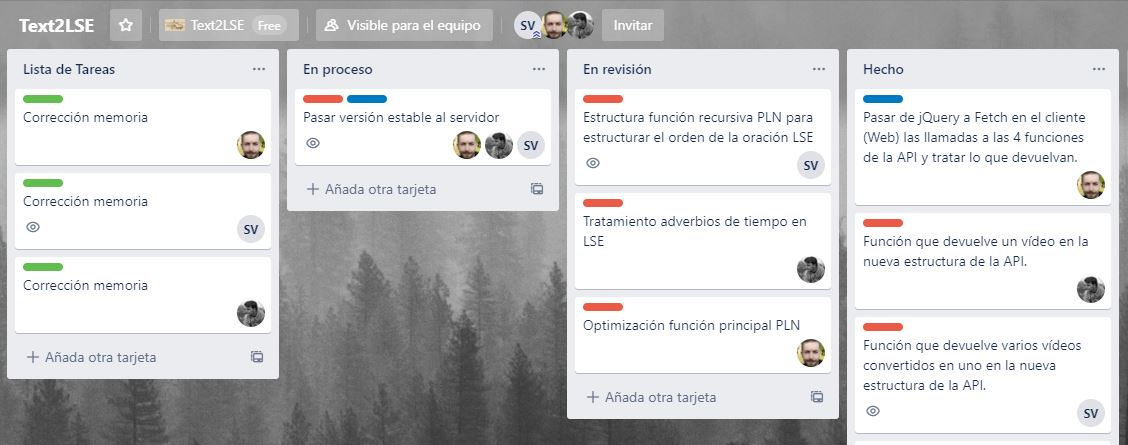
\includegraphics[width=1\textwidth]{Imagenes/Fuentes/Metodologias/trello.jpg}
	\caption{Tablero \textit{``Memoria''} utilizado en el proyecto.  }
	\label {fig: imgTrello}
\end{figure}
 


%-------------------------------------------------------------------
\section{Reuniones}
%-------------------------------------------------------------------
\label{cap4:sec:Reuniones}

Para una buena organizaci�n, desde el principio el equipo de trabajo se ha reunido una vez a la semana para asignar las diferentes tareas, comentar el trabajo realizado y poner en com�n todos los conocimientos adquiridos por cada uno. A lo largo de la semana tambi�n hab�a reuniones a trav�s de Skype\footnote {\url{https://www.skype.com/es/}} para comentar y resolver las posibles dudas que podr�an surgir durante el proceso. \\

El equipo tambi�n se ha mantenido en contacto v�a email con los tutores comentando el estado del proyecto. A esto se a�adieron reuniones mensuales con ellos para realizar correcciones de la memoria, revisar el progreso, resolver dudas y comentar las tareas necesarias para las siguientes fases.\\

De esta forma, los integrantes del equipo y los tutores han estado informados constantemente del progreso del trabajo, se ha podido hacer un reparto claro de tareas y se han podido establecer tiempos de entregas realistas y factibles.\\


%-------------------------------------------------------------------
\section{Control de versiones}
%-------------------------------------------------------------------
\label{cap4:sec:Control de versiones}
\subsection{GIT}

Para el desarrollo del proyecto se ha utilizado Git \footnote{Web oficial de Git \url{https://git-scm.com/}} que es un sistema de control de versiones distribuido que sirve para trabajar en equipo de una manera muy sencilla y optimizada. Git permite al usuario tener un control absoluto de su proyecto pudiendo ver todos los cambios realizados en nuestra aplicaci�n y nuestro c�digo por cada uno de los miembros o incluso volver a versiones anteriores del proyecto.

Sus principales herramientas son:

\begin{itemize}
	
	\item \textbf{Repository:} es un directorio donde se almacenan los archivos de tu proyecto. Puede estar ubicado en el almacenamiento de GitHub o en un repositorio local en tu computadora y tenerlos sincronizados.
	
	
	\item \textbf{Branch:} es una copia de tu repositorio cuyo desarrollo es independiente al repositorio central u otras ramas. Una vez realizados los cambios se puede combinar tu rama con otras ramas y con el repositorio central mediante un request.
	 
	
	\item \textbf{Commits:} son los cambios realizados en los archivos de tu repositorio local.

	\item \textbf{Pull:} acci�n que actualiza el repositorio local de tu ordenador con la �ltima versi�n del proyecto alojado en Github.
	
	\item \textbf{Push:} permite subir a Github los commits realizados en el repositorio local.	
	
\end{itemize}


\subsection{GITHUB}
GitHub \footnote{Web oficial de Github \url{https://help.github.com/}} es una plataforma que proporciona una interfaz que mediante las herramientas del control de versiones Git permite ver y llevar el registro de todos los cambios realizados en nuestro proyecto, organizarlos y resolver cualquier conflicto que pueda surgir. \\

Github tambi�n funciona como una red social para desarrolladores ya que permite a otros usuarios ver y colaborar en tus repositorios as� como resolver dudas que se tengan.






%---------------------------------------------------------------------
%
%                          Cap�tulo 5
%
%---------------------------------------------------------------------

\chapter{Text2LSE}


En este cap�tulo se describe el trabajo desarrollado a lo largo de este TFG. Text2LSE es una aplicaci�n web (ver Figura~\ref {fig: imgWebText2LSE}) que permite traducir textos escritos en castellano a LSE en formato texto LSE, v�deo e imagen en tiempo real. Text2LSE es una aplicaci�n p�blica, y se puede acceder a ella desde la siguiente url: 

\begin{shaded}
	\url{https://holstein.fdi.ucm.es/tfg-text2lse }	
\end{shaded}

Text2LSE sigue una arquitectura SOA y todos los servicios implementados est�n disponibles para todo el mundo de manera gratuita. Los v�deos e im�genes utilizados en la traducci�n a LSE son los recursos ofrecidos en el cat�logo de LSE de ARASAAC. \\

En la secci�n 5.1 se muestra la arquitectura de la aplicaci�n web y c�mo se comunica �sta con los servicios web. En la secci�n 5.2 se explican en profundidad los servicios web desarrollados, tanto los utilizados en la aplicaci�n web, como los desarrollados para aumentar las posibilidades de obtenci�n de informaci�n para futuros desarrolladores. Por �ltimo, en la secci�n 5.3 se detalla la aplicaci�n web, tanto su dise�o como su funcionalidad. \\


\begin{figure}[]
	\centering
	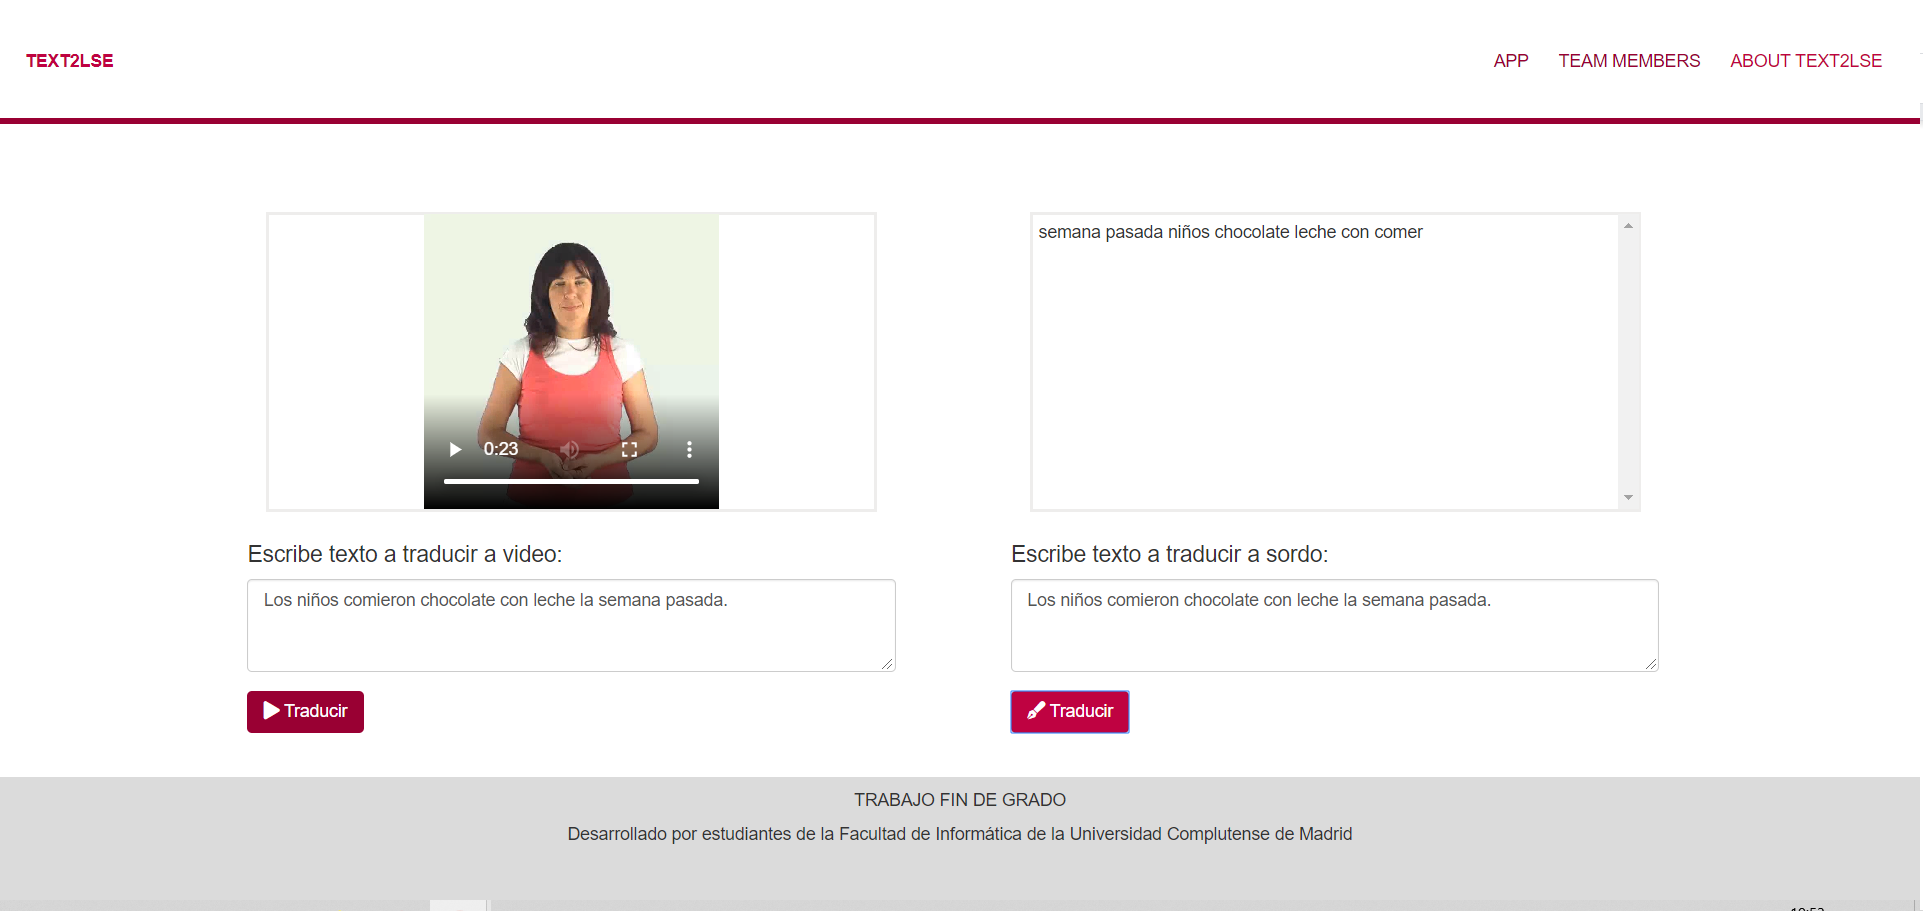
\includegraphics[width=1\textwidth]{Imagenes/Fuentes/Text2LSE/WebText2LSE.png}
	\caption{Aplicaci�n web Text2LSE }
	\label {fig: imgWebText2LSE}
\end{figure}

%-------------------------------------------------------------------
\section{Arquitectura}
%-------------------------------------------------------------------
\label{cap4:sec:Arquitectura}

Text2LSE es una aplicaci�n de traducci�n de castellano a LSE basada en servicios web, de manera que el c�digo desarrollado sea f�cilmente reutilizable. La arquitectura utilizada para el desarrollo de este proyecto es la arquitectura de cliente-servidor, es decir, un cliente muestra una web, la cual hace peticiones al servidor, que almacena los servicios web y devuelve la respuesta al cliente.\\

Se ha optado por desarrollar una aplicaci�n web debido a que �sta es accesible desde cualquier dispositivo que disponga de un navegador, ya sea un tel�fono m�vil, una tablet o un ordenador, sean de la marca y tama�o que sean. Para que se pueda ver de manera correcta en todos esos dispositivos, la aplicaci�n web se ha desarrollado siguiendo un dise�o responsive, es decir, que su visualizaci�n se adapte dependiendo de las dimensiones de la pantalla del dispositivo desde el cual se est� accediendo. La aplicaci�n web ha sido desarrollada usando html, css y javascript.\\

Respecto a la parte del servidor, se han desarrollado siete servicios web distintos: dos para devolver de manera r�pida el v�deo y la imagen en LSE de una sola palabra, otro para devolver el texto traducido a texto en LSE, dos para devolver el texto LSE para v�deos e im�genes y otros dos para devolver el texto traducido a video e im�genes en LSE. \\

Se ha utilizado un proxy inverso para poder acceder tanto a la p�gina web como a los servicios web a trav�s desde un mismo punto de acceso. Un Proxy inverso es un m�todo de redireccionamiento del tr�fico a partes espec�ficas de una infraestructura concreta\citep*{proxyInverso}. Las principales finalidades para las que se usa este tipo de servidores son:

\begin{itemize}
	
	\item \textbf{Anonimizaci�n:} el proxy recibe todas las llamadas al servidor y se encarga de filtrarlas y redirigirlas como se haya configurado previamente. De esta manera, desde fuera del servidor no se va a poder obtener ning�n tipo de informaci�n del servidor ni de los servicios que est�n en �l, solo se podr� obtener informaci�n del proxy.
	
	\item \textbf{Protecci�n y cifrado:} al utilizar un proxy inverso se tiene la posibilidad de instalar sistemas de control y filtros de paquetes que protegen al servidor, aumentando as� la seguridad del sistema.
	
	\item \textbf{Balanceo de carga:} permite redirigir las distintas solicitudes entrantes por varios servidores, permitiendo repartir la carga de trabajo para no sobrecargar ning�n servidor o equilibrar la carga en el caso de que falle uno de ellos.
	
	\item \textbf{Cach�:} el proxy se puede configurar para que sea capaz de almacenar las respuestas del servidor temporalmente para ofrecer una mayor velocidad de respuesta. De esta forma, si se recibe una solicitud cuya respuesta la tiene almacenada el proxy en su cach�, se manda la respuesta de manera inmediata haciendo que no reciba tanta carga de procedimiento el back-end.
	
	\item \textbf{Compresi�n:} un proxy inverso tambi�n se puede utilizar como compresor de datos, tanto entrantes como salientes.
	
\end{itemize}

En este proyecto, se ha configurado el servidor Nginx como servidor proxy inverso con el fin de redirigir las distintas solicitudes al servidor correspondientes. Se han especificado una serie de rutas para diferenciar qu� llamadas de usuario redireccionar a la p�gina web y cu�les a los servicios web. Esta estructura se puede observar en la Figura~\ref {fig: imgProxy}.

\begin{figure}[]
	\centering
	
	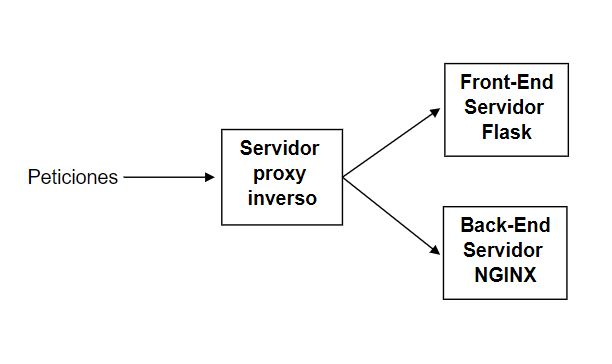
\includegraphics[width=1\textwidth]{Imagenes/Fuentes/Text2LSE/proxy.jpg}
	\caption{Esquema Proxy Inverso}
	\label {fig: imgProxy}
\end{figure}

\section{Back-End}

En esta secci�n se explican con detalle los servicios web desarrollados, su implementaci�n y c�mo utilizan de los recursos LSE de ARASAAC. La API donde est�n estos servicios es p�blica\footnote{\url{https://holstein.fdi.ucm.es/tfg-text2lse}} y en los siguientes apartados se indica la URL para acceder a cada servicio.


\subsection{Recursos LSE}

Todas las im�genes y v�deos LSE se han descargado del cat�logo de recursos de ARASAAC\footnote{\url{http://www.http://www.arasaac.org/descargas.php}}, que cuenta con 4.138 im�genes en formato jpg, y 4.102 v�deos en formato mp4. Estos recursos los hemos almacenado en dos carpetas alojadas en el propio servidor holstein: carpeta ``imagenes'' y carpeta ``videos''. Los servicios de traducci�n de palabra a v�deo LSE y a imagen LSE permiten obtener estos recursos mediante una llamada GET, en la cual se accede a la carpeta correspondiente y se busca el recurso con el nombre del signo buscado, concatenado con el formato que corresponda (jpg en el caso del servicio de traducci�n a imagen y mp4 en el de traducci�n a v�deo). Para crear la respuesta tanto en im�genes como en v�deo, se ha utilizado la funci�n \textit{``sendfile''} de Flask, que indicando como par�metro el fichero y su formato permite devolver archivos transformados en formato JSON.

\subsection{Servicio web de traducci�n de palabra a v�deo LSE }

Este servicio permite obtener el v�deo del signo en LSE correspondiente a una palabra en lenguaje natural. Para poder acceder a este servicio, se debe hacer una llamada GET a la API,  indicando la palabra que se desea traducir a LSE de la siguiente forma:\\

\begin{shaded}
	\url{https://holstein.fdi.ucm.es/tfg-text2lse/video/<palabra> }	
\end{shaded}

En el par�metro \textit{``palabra''} se debe indicar la palabra para la que se desea obtener su traducci�n en LSE. \\

Se utilizar� el par�metro de entrada para construir una ruta concatenando dicho par�metro con la ruta del directorio de v�deos del servidor. Esta ruta se utilizar� para comprobar la existencia del v�deo correspondiente. En caso de que exista, se usar� la funci�n \textit{``sendfile''} de Flask para devolverlo como respuesta, indicando como par�metro la ruta donde se aloja y su formato (mp4). En caso de que el v�deo buscado no exista, se sigue el mismo procedimiento, pero sustituyendo la ruta por la del v�deo de error. Este flujo lo podemos observar en la Figura~\ref {fig: imgFlujo1palabraText2LSE}. \\

Por ejemplo, para obtener el v�deo en LSE de la palabra \textit{``agua''} se debe realizar la siguiente llamada:

\begin{shaded}
	\url{https://holstein.fdi.ucm.es/tfg-text2lse/video/agua }	
\end{shaded}


\begin{figure}[]
	\centering
	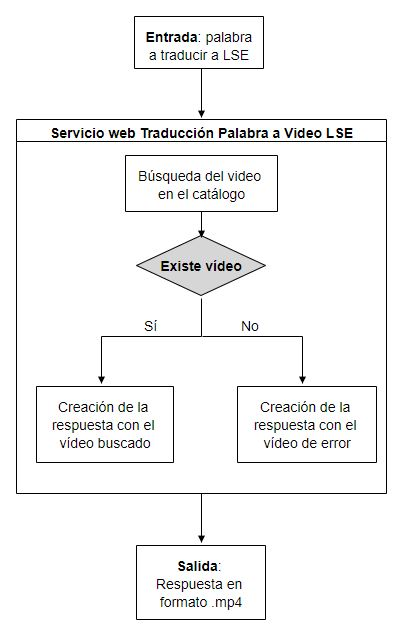
\includegraphics[width=0.7\textwidth]{Imagenes/Fuentes/Text2LSE/FlujoVideo1palabra.jpg}
	\caption{Flujo del servicio de Traducci�n de una palabra a v�deo en LSE}
	\label {fig: imgFlujo1palabraText2LSE}
\end{figure}

\subsection{Servicio web de traducci�n de palabra a imagen LSE }

Este servicio permite obtener la imagen del signo en LSE correspondiente a una palabra en lenguaje natural. Para poder acceder a este servicio, se debe hacer una llamada GET a la API,  indicando la palabra que se desea traducir a LSE de la siguiente forma:\\

\begin{shaded}
	\url{https://holstein.fdi.ucm.es/tfg-text2lse/imagen/<palabra> }	
\end{shaded}

En el par�metro \textit{``palabra''} se debe indicar la palabra de la que se desea obtener su traducci�n en LSE. \\

Se utilizar� el par�metro de entrada para construir una ruta concatenando dicho par�metro con la ruta del directorio de im�genes del servidor. Esta ruta se utilizar� para comprobar la existencia de la imagen correspondiente. En caso de que exista, se usar� la funci�n \textit{``sendfile''} de Flask para devolverlo como respuesta, indicando como par�metro la ruta donde se aloja y su formato (jpg). En caso de que la imagen buscada no exista, se sigue el mismo procedimiento, pero sustituyendo la ruta por la de la imagen de error, la cual la podemos observar en la Figura~\ref {fig: imgError}. Este flujo lo podemos observar en la Figura~\ref {fig: imgFlujo1palabraImagenText2LSE}. \\

Por ejemplo, para obtener la imagen en LSE de la palabra \textit{``coche''} se debe realizar la siguiente llamada:

\begin{shaded}
	\url{https://holstein.fdi.ucm.es/tfg-text2lse/imagen/coche }	
\end{shaded}

La respuesta a la llamada del ejemplo devolver� la imagen de la Figura~\ref {fig: imgCoche}.

\begin{figure}[]
	\centering
	
\includegraphics[width=0.5\textwidth]{Imagenes/Fuentes/Text2LSE/imgError.jpg}
	\caption{Imagen de error devuelta en la traducci�n de una palabra a LSE}
	\label {fig: imgError}
\end{figure}

\begin{figure}[]
	\centering
	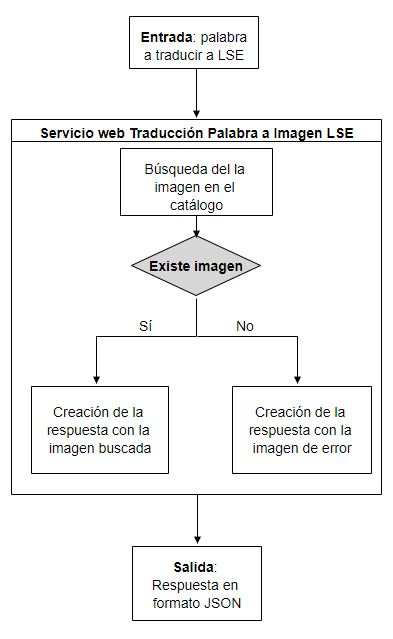
\includegraphics[width=0.7\textwidth]{Imagenes/Fuentes/Text2LSE/FlujoImagen1palabra.jpg}
	\caption{Flujo del servicio de Traducci�n de una palabra a imagen en LSE}
	\label {fig: imgFlujo1palabraImagenText2LSE}
\end{figure}

\begin{figure}[]
	\centering
	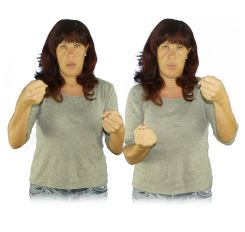
\includegraphics[width=0.5\textwidth]{Imagenes/Fuentes/Text2LSE/imagenEjemplo.jpg}
	\caption{Imagen devuelto por el servicio de traducci�n de la palabra \textit{``coche''} a LSE}
	\label {fig: imgCoche}
\end{figure}


\subsection{Servicio web para Traducci�n de texto en castellano a texto en LSE}
Este servicio implementa la funcionalidad de traducci�n de un texto en castellano a LSE en formato texto.
Para poder acceder a este servicio, se debe realizar una petici�n POST a la API en la siguiente URL:

\begin{shaded}
	\url{https://holstein.fdi.ucm.es/tfg-text2lse/TextoLSE}	
\end{shaded}


Los datos a enviar en la petici�n POST deben tener la siguiente estructura en JSON: 
\begin{center}
	
	\{ 'Texto' : '<texto>' \}
	
\end{center}

En el par�metro ``texto'' se debe incluir el texto que se desea traducir a LSE. Un ejemplo de uso ser�a: 



\begin{center}
	Entrada:  \{ ``Texto'' : ``El ni�o bebe agua.'' \}\\
	Salida:   \{ ``Texto'' : ``ni�o agua beber.'' \}
\end{center}


El flujo de este servicio web lo podremos ver en la Figura~\ref {fig: imgFlujoFlujoTextoLSE}.


\begin{figure}[]
	\centering
	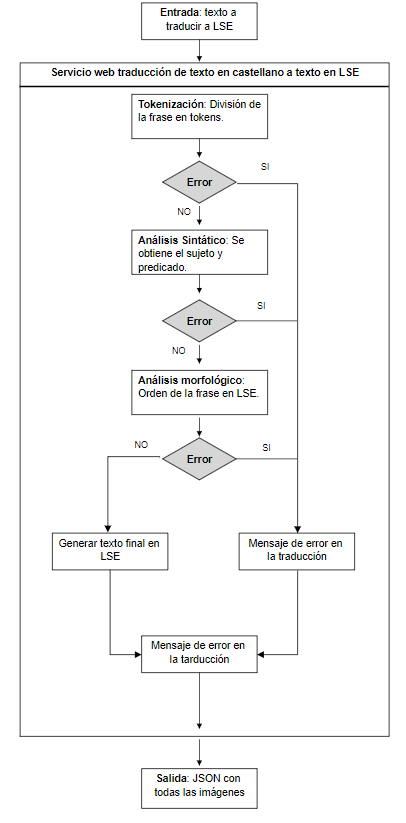
\includegraphics[width=1\textwidth]{Imagenes/Fuentes/Text2LSE/textotextoLSE.png}
	\caption{ Flujo servicio de traducci�n de texto en castellano a texto en LSE }
	\label {fig: imgFlujoFlujoTextoLSE}
\end{figure}

Para que el servicio web sea capaz de traducir una frase a LSE se ha tenido que realizar un procesamiento previo del texto en castellano para poder adaptarlo a la Lengua de Signos Espa�ola.


Este procesamiento es realizado con sistema de reglas las cuales filtran qu� palabras deben de ser utilizadas y cuales no al igual que determina su orden en la oraci�n en LSE. La elecci�n a la hora de desarrollar el Procesamiento del Lenguaje Natural para nuestro proyecto estaba entre un sistema basado en reglas o mediante el uso de aprendizaje autom�tico. La opci�n de desarrollar un aprendizaje autom�tico no era viable debido a la dificultad y la falta de ejemplos en castellano para entrenar el sistema. Por este motivo se eligi� el sistema basado en reglas ya que era m�s f�cil de implementar y aunque puede limitar la capacidad de traducci�n de frases que no cumplan dichas reglas, cumple con los objetivos marcados en el proyecto que es traducir frases simples a LSE.\\

Nuestro PLN se divide en tres fases. Lo primero que hace es recopilar informaci�n de la frase para luego realizar un an�lisis sint�ctico y morfol�gico de la frase y as� poder ordenarla respetando la estructura de la LSE. A continuaci�n se explicar� con m�s detalle cada una de las fases:

\subsubsection{Tokenizaci�n} 
Para poder realizar el an�lisis sint�ctico y morfol�gico de la frase se necesita obtener toda la informaci�n posible de la frase. Para ello se realizar� el proceso de tokenizaci�n el cual divide la frase en una lista de palabras denominadas \textit{tokens} donde cada token contiene la siguiente informaci�n de cada palabra:


\begin{itemize}
	
	\item \textbf{Dependencia:} Indica la relaci�n de dependencia sint�ctica dentro de la oraci�n, es decir, que funci�n tiene la palabra dentro de la oraci�n donde las m�s importantes son sujeto, ra�z u objeto.
	\item \textbf{Tags:} Indica el g�nero, n�mero, el tiempo verbal y la persona de cada token.
	\item \textbf{Part of speech:} Indica el tipo de palabra en funci�n de su uso en la oraci�n, tales como nombres, adjetivos, adverbios y verbos.
	\item \textbf{Lemma:} Indica el lema de una palabra,es decir, la palabra que se encuentra al frente del diccionario por ejemplo, El lemma de ``jug�bamos'' es ``jugar''
	
\end{itemize}


Por ejemplo los tokens que aparecen en \textit{`Los ni�os merendaron chocolate'} ser�a los que aparecen en la Figura ~\ref {fig: tokenInformacion}:
\begin{figure}[h]
	\centering
	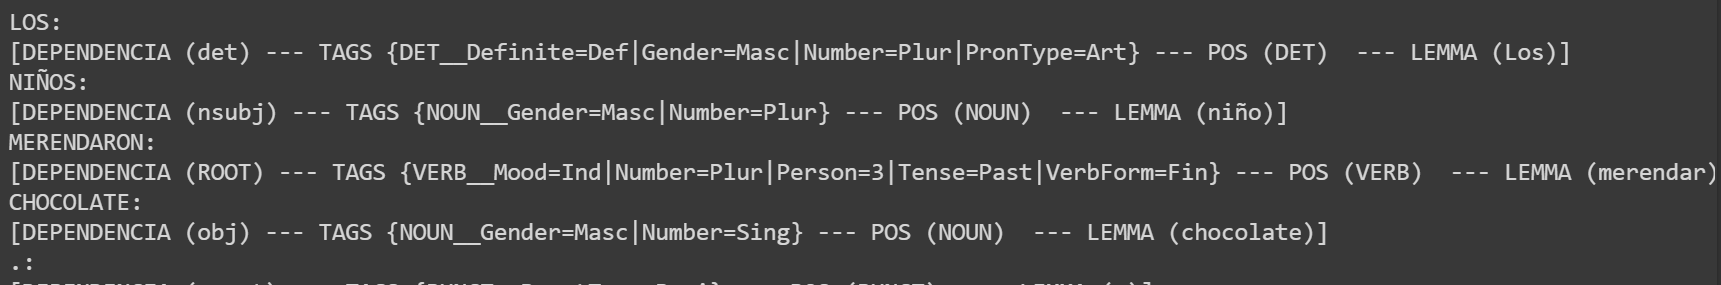
\includegraphics[width=1 \textwidth]{Imagenes/Fuentes/PNL/InfoPLN.png}
	\caption{ Tokens de la frase ``Los ni�os meredaron chocolate'' }
	\label {fig: tokenInformacion}
\end{figure}

Como se ve en la Figura ~\ref {fig: tokenInformacion} cada token tiene su informaci�n detallada. Por ejemplo de los tokens \textit{``los''} y \textit{``ni�os''} la informaci�n obtenida ser�a:
\begin{itemize}
	\item \textbf{Los:} la dependencia indica que es un determinante y los tags que es art�culo determinado, masculino y plural. 
	\item \textbf{ni�os:} la dependencia indica que es el sujeto de la oraci�n, los tags que es masculino y plural y el lemma proporciona la palabra que vendr�a en el diccionario.  
	
\end{itemize}

Mediante la tokenizaci�n a parte de poder obtener la informaci�n de cada palabra se obtiene un �rbol de dependencias entre palabras. Para entender c�mo funcionan las dependencias se va a utilizar como ejemplo la oraci�n `Ayer los ni�os merendaban chocolate' donde sus dependencias se muestran en la Figura ~\ref {fig: dependencias} 

\begin{figure}[h]
	\centering
	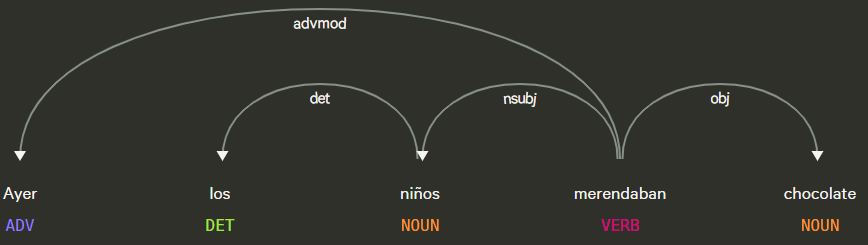
\includegraphics[width=1\textwidth]{Imagenes/Fuentes/Text2LSE/dependencias.png}
	\caption{ Displacy grafo de dependencias }
	\label {fig: dependencias}
\end{figure}

Como se puede apreciar en el diagrama del token `merendaban' dependen tres tokens (Ayer, ni�os y chocolate) y de ellos tambi�n dependen otros y as� sucesivamente. Estas dependencias se traducen en un �rbol donde el ROOT es la ra�z como podemos ver en la Figura~\ref {fig: grafo}:\\


\begin{figure}[]
	\centering
	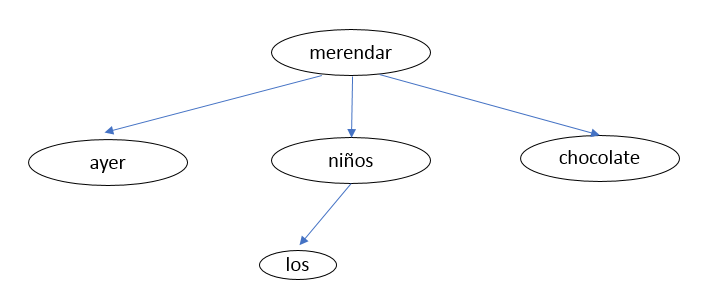
\includegraphics[width=1\textwidth]{Imagenes/Fuentes/Text2LSE/grafo.png}
	\caption{ �rbol de ls oraci�n ``Los ni�os merendaron chocolate'' }
	\label {fig: grafo}
\end{figure}



\subsubsection{An�lisis sint�ctico} 
Una vez separado la oraci�n en tokens hay que diferenciar que palabras forman parte del sujeto y cuales del predicado. Para ello hay que recorrer el �rbol de dependencias mediante una funci�n recursiva empezando desde el ROOT que es el token ra�z del cual dependen todos los dem�s.\\

Para obtener el sujeto se busca el token que contenga la dependencia ``nsuj''. A continuaci�n se obtienen los hijos del token ``nsuj'' y se guardan como parte del sujeto mientras que los tokens restantes, es decir, aquellos que no pertenecen al sujeto formar�an parte del predicado. En el ejemplo anterior \textit{``Ayer los ni�os merendaban chocolate''} el \textbf{sujeto} ser�a \textit{``Los, ni�os''} y el \textbf{predicado} \textit{``Ayer, merendaban y chocolate''}.\\

El resultado de los tokens pertenecientes al sujeto y al predicado se almacena en una lista
\begin{center}
	\begin{itemize}
		\item \textbf{Sujeto:}  [Los, ni�os]
		\item \textbf{Predicado:} [Ayer, merendaban, chocolate]
		
	\end{itemize}
\end{center}

\subsubsection{An�lisis morfol�gico} 

La Lengua de Signos Espa�ola tiene una estructura gramatical diferente al castellano. Para comenzar con la traducci�n se toma como punto de partida la estructura m�s simple en LSE: 
\begin{center}
	TIEMPO + SUJETO + OBJETO + VERBO.
\end{center}

Como se explica en la secci�n ~\ref {cap2:sec:Sintaxis de la Lengua de Signos} en la LSE las palabras pueden estar estructuradas de forma diferente con respecto a la oraci�n original en castellano.


Para conseguir la traducci�n de la frase original en castellano a LSE se necesita un an�lisis morfol�gico que permita detectar:

\begin{itemize}
	
	\item \textbf{Determinantes:} Los determinantes se omiten a la hora de hacer la traducci�n \textit{por ejemplo, ``El ni�o come carne''} se traduce como \textit{``Ni�o carne comer''.}
	
	\item \textbf{Verbos copulativos:} Los verbos copulativos ser, estar o parecer se omiten a la hora de la traducci�n \textit{por ejemplo, ``yo soy bajo''} se traduce como \textit{``yo bajo''.}
	
	\item \textbf{Posesivos:} Los determinantes posesivos se sustituyen por pronombres personales \textit{por ejemplo, ``Mi ni�o es bajo''} se traduce como \textit{``yo ni�o bajo''.}
	
	\item \textbf{Preposiciones:} Algunas preposiciones se quitan y otras se a�aden \textit{por ejemplo, ``Mi ni�o est� en el parque''} se traduce como \textit{``yo hijo parque''.} o \textit{por ejemplo, ``yo jugaba con el perro''} se traduce como \textit{``yo perro jugar''.}
	
	\item \textbf{Adjetivos:} Los adjetivos se ponen en masculino\textit{por ejemplo, ``Mi mam� es fea''} se traduce como \textit{``yo mam� feo''.}
	
	\item \textbf{Temporalidad:} La temporalidad va al principio de la oraci�n. \textit{por ejemplo, ``Yo com� chocolate ayer''} se traduce como \textit{``Ayer yo chocolate comer''.} Sin embargo no siempre hay adverbios de tiempo en la oraci�n que indican la temporalidad, en este caso el tiempo viene determinado por el tiempo verbal \textit{por ejemplo, ``Yo comer� chocolate''} se traduce como \textit{``Futuro yo chocolate comer''.}
	
	
	
\end{itemize}


Una vez a�adido y quitado las palabras el sujeto y predicado, la frase se tiene que ordenar seg�n la estructura tiempo + sujeto + objeto + verbo por lo que el resultado final de la frase usada como ejemplo ``Los ni�os ayer merendaban chocolate'' ser�a: 

\begin{center}
	\begin{itemize}
		\item \textbf{Sujeto:}  [ni�os]
		\item \textbf{Predicado:} [Ayer, merendar, chocolate]
		\item \textbf{Frase ordenada:} ``Ayer ni�os chocolate merendar'' 
		
		
	\end{itemize}
\end{center}

\subsection{Servicio web de traducci�n de texto en LN a texto LSE adaptado al cat�logo de v�deos de ARASAAC }
\label{cap5:sec:textoLSEvideo}

Este servicio implementa la funcionalidad de traducci�n de un texto en castellano a LSE en formato texto en funci�n de los v�deos existentes en el cat�logo de ARASAAC. Para poder acceder a este servicio, se debe realizar la siguiente petici�n POST a la API:\\

\begin{shaded}
	\url{https://holstein.fdi.ucm.es/tfg-text2lse/TextoLSEVideos/  }	
\end{shaded}


Los datos a enviar en la petici�n POST deben tener la siguiente estructura en JSON: 
\begin{center}
	
	\{ `Texto' : `<texto>' \}
	
\end{center}


En el par�metro \textit{``texto''} se debe incluir el texto que se desea traducir a LSE. Al recibir este par�metro, este servicio lo utilizar� para hacer una llamada al servicio de traducci�n de texto en LN a texto LSE, con el fin obtener la traducci�n a texto LSE. Una vez obtenida esta traducci�n, se realizar�n una serie de comprobaciones y transformaciones por cada palabra que sea un sustantivo, con la finalidad de adaptarlas al cat�logo de v�deos de ARASAAC. Para comenzar, se comprueba si existe v�deo para ese sustantivo, y en caso de que exista se pasa a comprobar la siguiente palabra. Si por el contrario no existe el v�deo, se eliminan los morfemas de g�nero y n�mero, y se vuelve a comprobar si existe el v�deo. Si tras este cambio sigue sin existir el v�deo, se deja la palabra sin modificar y se pasa a comprobar la siguiente. Si existe v�deo tras el cambio, se comprueba si la palabra era femenina y si es as� se a�ade a continuaci�n la palabra \textit{``FEMENINO''}. Despu�s se comprueba si la palabra estaba en plural y si es as� se a�ade a continuaci�n la palabra \textit{``PLURAL''}. Al realizar estas comprobaciones con todas las palabras, se crea la respuesta en formato JSON y se devuelve. El flujo de este servicio lo podemos observar en la Figura~\ref {fig: imgFlujoTextoVideoTextoText2LSE}.\\

Por ejemplo, para traducir el texto \textit{``Mis t�as comen chocolate''} a LSE en formato texto en funci�n de los v�deos existentes, se debe realizar la llamada POST indicada anteriormente con el siguiente JSON:


\begin{center}
	Entrada: \{ `Texto' : `Mis t�as comen chocolate' \} \\
\end{center}

Al no existir el v�deo para la palabra \textit{``t�as''}, busca el v�deo de esa palabra sin morfemas de g�nero y n�mero, que en este caso es la palabra \textit{``t�o''}. Como \textit{``t�as''} es plural y femenino, se a�aden las palabras  \textit{``FEMENINO''} para indicar el femenino y \textit{``PLURAL''} para indicar el plural. Para finalizar, se crea la respuesta en formato JSON y se devuelve. La salida en este caso ser�a:

\begin{center}
	Salida: \{ `Texto' : `YO T�O FEMENINO PLURAL CHOCOLATE COMER' \}
\end{center}

\begin{figure}[]
	\centering
	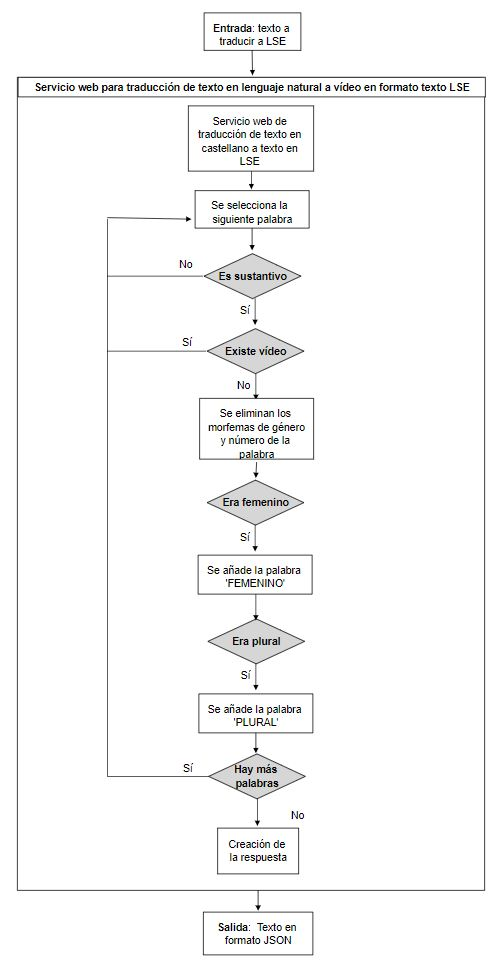
\includegraphics[width=0.8\textwidth]{Imagenes/Fuentes/Text2LSE/FlujoTextoVideoTexto.jpg}
	\caption{ Flujo servicio web de traducci�n de texto en LN a texto LSE adaptado al cat�logo de v�deos de ARASAAC }
	\label {fig: imgFlujoTextoVideoTextoText2LSE}
\end{figure}

\subsection{Servicio web de traducci�n de texto en LN a texto LSE adaptado a las im�genes del cat�logo de ARASAAC}

Este servicio implementa la funcionalidad de traducci�n de un texto en castellano a LSE en formato texto en funci�n de las im�genes existentes en el sistema. Para poder acceder a este servicio, se debe realizar la siguiente petici�n POST a la API:\\

\begin{shaded}
	\url{https://holstein.fdi.ucm.es/tfg-text2lse/textoImagen/  }	
\end{shaded}


Los datos a enviar en la petici�n POST deben tener la siguiente estructura en JSON: 
\begin{center}
	
	\{ `Texto' : `<texto>' \}
	
\end{center}


En el par�metro \textit{``texto''} se debe incluir el texto que se desea traducir a LSE. Al recibir este par�metro, este servicio lo utilizar� para hacer una llamada al servicio de traducci�n de texto en LN a texto LSE, con el fin obtener la traducci�n a texto LSE. Una vez obtenida esta traducci�n, se realizar�n una serie de comprobaciones y transformaciones por cada palabra que sea un sustantivo, con la finalidad de adaptarlas al cat�logo de im�genes de ARASAAC. Para comenzar, se comprueba si existe la imagen para ese sustantivo, y en caso de que exista se pasa a comprobar la siguiente palabra. Si por el contrario no existe la imagen, se eliminan los morfemas de g�nero y n�mero, y se vuelve a comprobar si existe la imagen. Si tras este cambio sigue sin existir la imagen, se deja la palabra sin modificar y se pasa a comprobar la siguiente. Si existe la im�gen tras el cambio, se comprueba si la palabra era femenina y si es as� se a�ade a continuaci�n la palabra \textit{``FEMENINO''}. Despu�s se comprueba si la palabra estaba en plural y si es as� se a�ade a continuaci�n la palabra \textit{``PLURAL''}. Al realizar estas comprobaciones con todas las palabras, se crea la respuesta en formato JSON y se devuelve. El flujo de este servicio lo podemos observar en la Figura~\ref {fig: imgFlujoTextoImagenTextoText2LSE}.\\

Por ejemplo, para traducir el texto \textit{``Los caballos son r�pidos''} a LSE en formato texto en funci�n de las im�genes existentes, se debe realizar la llamada POST indicada anteriormente con el siguiente JSON:


\begin{center}
	Entrada: \{ `Texto' : `Los caballos son r�pidos' \} 
\end{center}

Al no existir la imagen para la palabra  \textit{``caballos''}, busca la imagen de esa palabra sin morfemas de g�nero y n�mero, que en este caso es la palabra \textit{``caballo''}. Como \textit{``caballos''} es plural, se a�ade la palabra \textit{``PLURAL''} para indicar el plural. Para finalizar, se crea la respuesta en formato JSON y se devuelve. La salida en este caso ser�a:
 
\begin{center}
	Salida: \{ `Texto' : `CABALLO PLURAL R�PIDO' \}
\end{center}

\begin{figure}[]
	\centering
	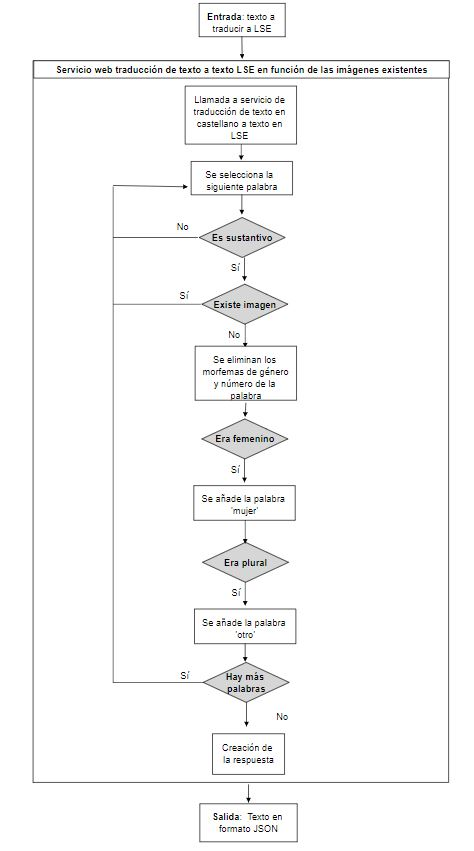
\includegraphics[width=0.8\textwidth]{Imagenes/Fuentes/Text2LSE/FlujoTextoImagenTexto.jpg}
	\caption{ Flujo servicio web de traducci�n de texto en LN a texto LSE adaptado al cat�logo de im�genes de ARASAAC}
	\label {fig: imgFlujoTextoImagenTextoText2LSE}
\end{figure}


\subsection{Servicio web para traducci�n de texto a LSE (v�deo)}
\label{cap5:sec:textoLSEvideoCompleto}

Este servicio implementa la funcionalidad de traducci�n de un texto en castellano a LSE en formato video.  Para poder acceder a este servicio, se debe realizar la siguiente petici�n POST a la API:\\

\begin{shaded}
	\url{https://holstein.fdi.ucm.es/tfg-text2lse/video/  }	
\end{shaded}


Los datos a enviar en la petici�n POST deben tener la siguiente estructura en JSON: 
\begin{center}

		\{ 'Texto' : '<texto>' \}

\end{center}


En el par�metro \textit{``texto''} se debe incluir el texto que se desea traducir a LSE. Al recibir este par�metro, este servicio lo utilizar� para hacer una llamada al servicio de traducci�n de texto en LN a texto LSE adaptado al cat�logo de v�deos de ARASAAC, con el fin obtener la traducci�n a texto LSE. Una vez obtenida esta traducci�n, por cada palabra se llamar� al servicio de traducci�n de palabra a v�deo LSE, que devolver� el video correspondiente o el v�deo de error en caso de que no exista el video buscado. Al finalizar con todas las palabras se utilizar� la libreria Moviepy\footnote{\url{https://zulko.github.io/moviepy/index.html}} de Python para concatenar todos v�deos recibidos en uno solo, que se devolver� como respuesta. El flujo de este servicio lo podemos observar en la Figura~\ref {fig: imgFlujoVideoTextoText2LSE}.\\

Por ejemplo, para obtener el v�deo en LSE del texto \textit{``Los ni�os comen chocolate''}, se debe realizar la llamada POST indicada anteriormente con el siguiente JSON:

\begin{center}
	
	\{ `Texto' : `Los ni�os comen chocolate' \}
	
\end{center}

La respuesta recibida ser� un �nico v�deo en formato mp4 con la traducci�n deseada.

\begin{figure}[]
	\centering
	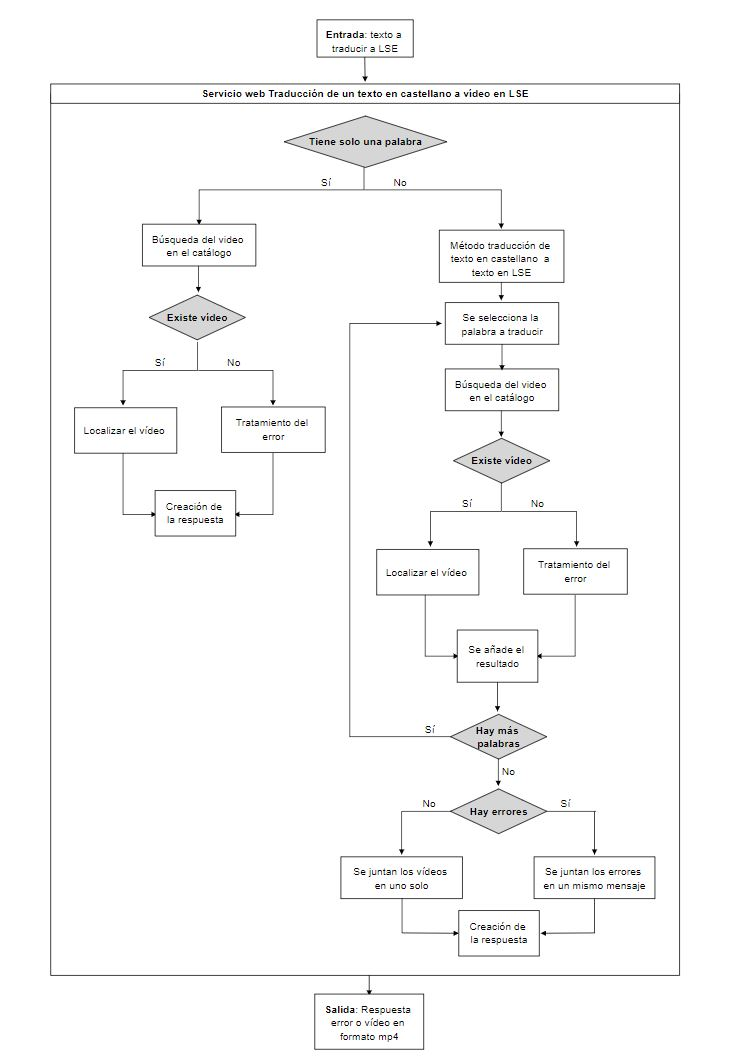
\includegraphics[width=1\textwidth]{Imagenes/Fuentes/Text2LSE/FlujoVideoTexto.jpg}
	\caption{ Flujo del servicio web para traducci�n de texto a LSE (v�deo) }
	\label {fig: imgFlujoVideoTextoText2LSE}
\end{figure}




\subsection{Servicio web para traducci�n de texto a LSE (imagen)}

Este servicio implementa la funcionalidad de traducci�n de un texto en castellano a LSE en formato imagen. Para poder acceder a este servicio, se debe realizar la siguiente petici�n POST a la API:\\

\begin{shaded}
	\url{https://holstein.fdi.ucm.es/tfg-text2lse/imagenes/  }	
\end{shaded}

Los datos a enviar en la petici�n POST deben tener la siguiente estructura en JSON:

\begin{center}
	
	\{ 'Texto' : '<texto>' \}
	
\end{center}


En el par�metro \textit{``texto''} se debe incluir el texto que se desea traducir a LSE. Al recibir este par�metro, este servicio lo utilizar� para hacer una llamada al servicio de traducci�n de texto en LN a texto LSE adaptado al cat�logo de im�genes de ARASAAC, con el fin obtener la traducci�n a texto LSE. Una vez obtenida esta traducci�n, por cada palabra se llamar� al servicio de traducci�n de palabra a imagen LSE, que devolver� la ruta de la imagen correspondiente o la ruta de la imagen de error en caso de que no exista la imagen buscada. Al finalizar con todas las palabras se a�adir�n sus rutas en orden en un array JSON que se devolver� como respuesta. El flujo de este servicio lo podemos observar en la Figura~\ref {fig: FlujoImagenTexto}.\\

Por ejemplo, para obtener las im�genes en LSE del texto \textit{``Ma�ana yo ir� al m�dico''}, se debe realizar la llamada POST indicada anteriormente con el siguiente JSON:

\begin{center}
	
	\{ `Texto' : `Ma�ana yo ir� al m�dico' \}
	
\end{center}

La respuesta recibida ser� un JSON que contendr� un array con todas las rutas de las im�genes, como podemos ver a continuaci�n en la Figura \ref{fig: jsonImagenes}. 




\begin{figure}[]
	\centering
	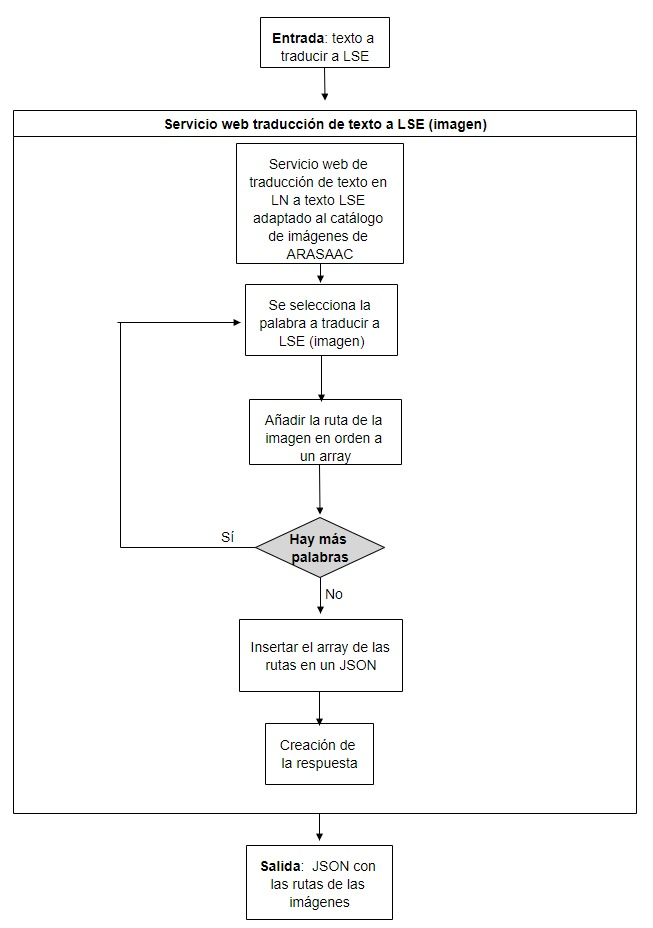
\includegraphics[width=1\textwidth]{Imagenes/Fuentes/Text2LSE/FlujoImagenText.jpg}
	\caption{ Flujo del servicio web para traducci�n de texto a LSE (imagen) }
	\label {fig: FlujoImagenTexto}
\end{figure}

\begin{figure}[]
	\centering
	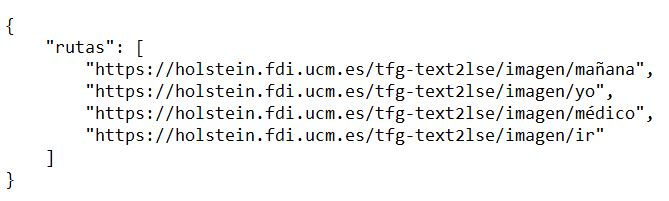
\includegraphics[width=1\textwidth]{Imagenes/Fuentes/Text2LSE/arrayImagenes.jpg}
	\caption{ JSON devuelto por el servicio web para traducci�n de texto a LSE (imagen) }
	\label {fig: jsonImagenes}
\end{figure}


\section{Front-End}

En esta secci�n se explica en detalle la aplicaci�n web desarrollada, cuya finalidad es proporcionar a los usuarios una interfaz sencilla donde puedan introducir el texto que desean traducir y obtener la traducci�n del texto en LSE, tanto en im�genes como en v�deo. En la  Figura~\ref {fig: imgWebText2LSE} se muestra la interfaz de la aplicaci�n, que consta de un input donde el usuario podr� introducir el texto en castellano que desee traducir, un desplegable donde podr� seleccionar el formato de salida y un bot�n para realizar la traducci�n.\\

Los formatos de salida disponibles en el desplegable son los siguientes:

\begin{itemize}

	\item \textbf{Traducci�n a v�deo:} tras seleccionar este formato y pulsar el bot�n ``traducir'', se realizar� una llamada Fetch al servicio web de traducci�n de texto en lenguaje natural a texto LSE (ver secci�n \ref{cap5:sec:textoLSEvideo}), pasando por el servidor proxy, que a su vez redirigir� la petici�n a la API. Una funci�n Fetch se encargar� de recibir el texto resultante y de llamar por cada una de esas palabras al servicio que devuelve el video LSE correspondiente. Posteriormente se incrustan todos los v�deos en orden en el c�digo HTML, de tal manera que se reproduce uno detr�s de otro. As�, se podr� visualizar por pantalla un v�deo en el que se podr� ver a un int�rprete de ARASAAC realizando los signos LSE correspondientes. En la Figura~\ref {fig: esquemaTradVideo} se puede observar el flujo para la traducci�n en este formato. Se ha decididohacerlo as� en lugar de llamar directamente servicio de traducci�n de texto a LSE (v�deo), explicado en la secci�n \ref{cap5:sec:textoLSEvideoCompleto}, porque el tiempo de respuesta de ese servicio web es largo y supone una gran carga de trabajo para el servidor concatenar v�deos mp4 y devolverlos como respuesta.
	

	
	\item \textbf{Traducci�n a im�genes:} de la misma manera que en el caso de los v�deos, tras seleccionar este formato y pulsar el bot�n ``traducir'', se realizar� una llamada Fetch  al servicio web de traducci�n de texto en lenguaje natural a texto LSE adaptado al cat�logo de im�genes de ARASAAC, pasando por el servidor proxy, que a su vez redirigir� la petici�n a la API. Una funci�n Fetch se encargar� de recibir el texto resultante y de llamar por cada una de esas palabras al servicio que devuelve la imagen LSE correspondiente. Posteriormente se incrustan todas las im�genes en orden en el c�digo HTML. En la Figura~\ref {fig: esquemaTradImagen} se puede observar el flujo para la traducci�n a im�genes.

	\item \textbf{Traducci�n a texto LSE:} tras seleccionar este formato y pulsar el bot�n ``traducir'' se llamar� a una funci�n Fetch que realizar� una petici�n al servicio de traducci�n de texto en castellano a texto en LSE. En caso de �xito aparecer� por pantalla dicho texto traducido a texto LSE. En la Figura~\ref {fig: esquemaTradTexto} se puede observar el flujo para esta traducci�n.

\end{itemize}


\begin{figure}[]
	\centering
	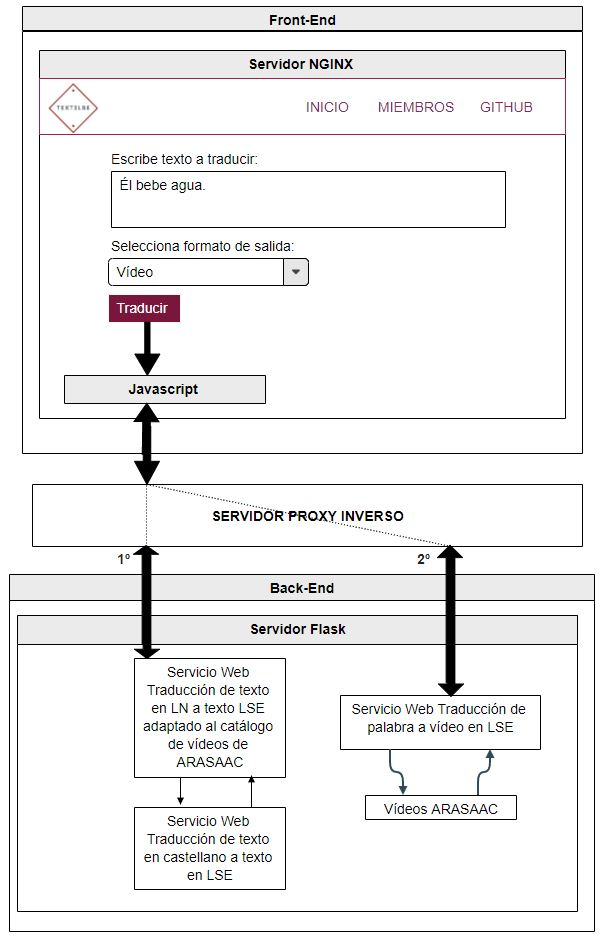
\includegraphics[width=1\textwidth]{Imagenes/Fuentes/Text2LSE/esquemaTradVideo.jpg}
	\caption{ Flujo de la aplicaci�n web al seleccionar la traducci�n en formato v�deo. }
	\label {fig: esquemaTradVideo}
\end{figure}

\begin{figure}[]
	\centering
	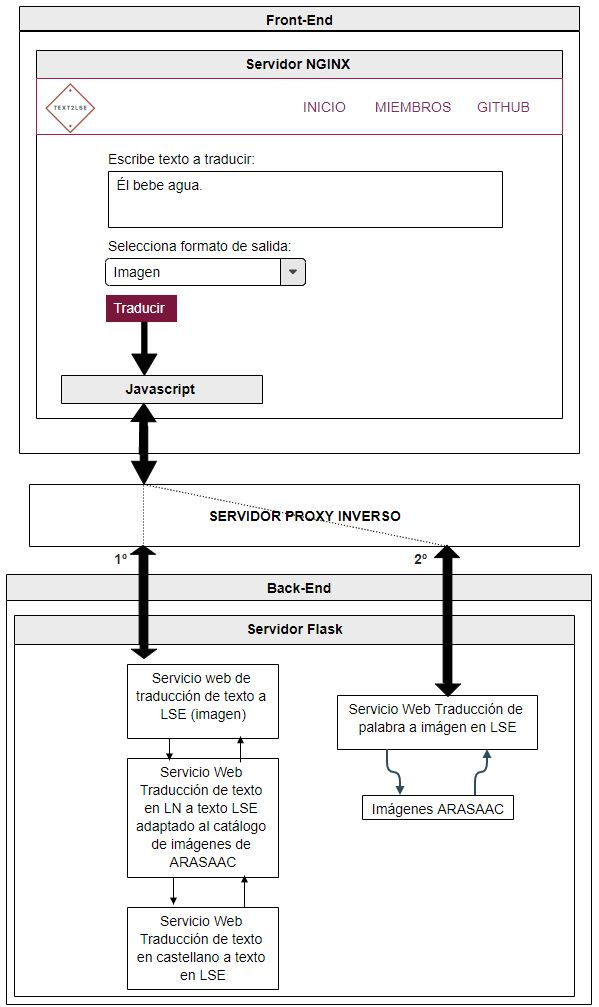
\includegraphics[width=1\textwidth]{Imagenes/Fuentes/Text2LSE/esquemaTradImagen.jpg}
	\caption{ Flujo de la aplicaci�n web al seleccionar la traducci�n en formato imagen. }
	\label {fig: esquemaTradImagen}
\end{figure}


\begin{figure}[]
	\centering
	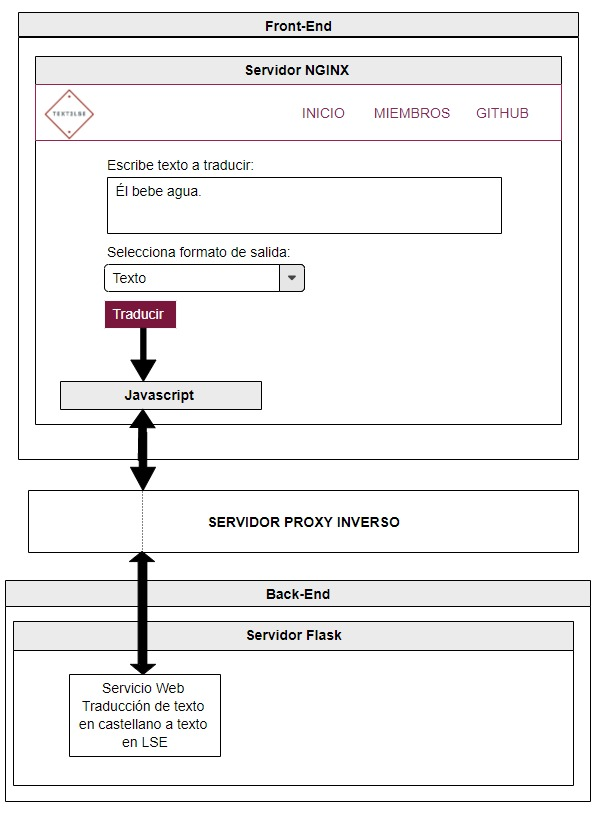
\includegraphics[width=1\textwidth]{Imagenes/Fuentes/Text2LSE/esquemaTradTexto.jpg}
	\caption{ Flujo de la aplicaci�n web al seleccionar la traducci�n en formato texto.}
	\label {fig: esquemaTradTexto}
\end{figure}

En caso de error en cualquiera de las tres funcionalidades, la aplicaci�n mostrar� un modal con el tipo y detalle del error obtenido al realizar la petici�n a la API donde se encuentran nuestros servicios web.\\ 

Por otro lado, la interfaz tambi�n cuenta con un men� en la parte superior, donde adem�s de a la p�gina principal podemos acceder a una p�gina con informaci�n sobre los miembros del equipo y de los tutores, y a otra con informaci�n sobre la aplicaci�n.\\ 

Toda la aplicaci�n se ha implementado siguiendo un dise�o responsive, haciendo uso de Bootstrap 3, para garantizar que la herramienta sea accesible desde cualquier dispositivo. En la Figura~\ref {fig: imgResponsive} podemos observar la interfaz vista desde un dispositivo m�vil.\\


\begin{figure}[H]
	\centering
	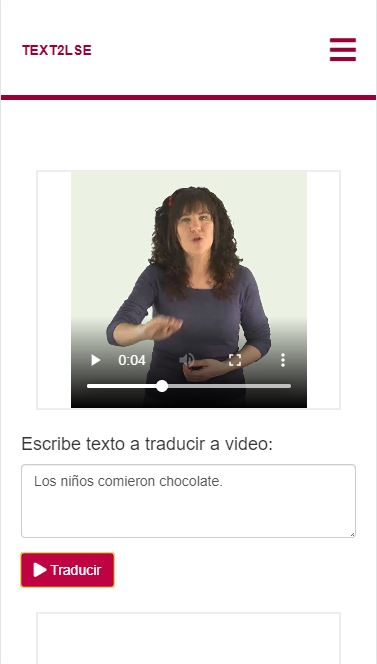
\includegraphics[width=0.6\textwidth]{Imagenes/Fuentes/Text2LSE/responsive.jpg}
	\caption{ Aplicaci�n Web vista desde un dispositivo m�vil }
	\label {fig: imgResponsive}
\end{figure}




%---------------------------------------------------------------------
%
%                          Cap�tulo 6
%
%---------------------------------------------------------------------

\chapter{Evaluaci�n}

Al terminar la fase de desarrollo, comenz� la fase de evaluaci�n, cuya finalidad era comprobar la correcci�n del trabajo realizado y la precisi�n y alcance de las traducciones, para la cual se usar�n m�tricas y se realizar� un an�lisis cualitativo. En este cap�tulo se muestra el proceso de dicha evaluaci�n para poder determinar qu� tipo de oraciones se logra traducir y con qu� nivel de fiabilidad. En la Secci�n \ref{cap6:sec:Dise�o de la evaluaci�n} se explica el dise�o de la evaluaci�n realizada, en la Secci�n \ref{cap6:sec:Resultados de la Evaluaci�n} se presentan los resultados y en la Secci�n \ref{cap6:sec:An�lisis de los Resultados} se realiza el an�lisis y discusi�n de los resultados obtenidos.

%-------------------------------------------------------------------
\section{Dise�o de la evaluaci�n}
%-------------------------------------------------------------------
\label{cap6:sec:Dise�o de la evaluaci�n}

Hemos enfocado la fase de evaluaci�n en la precisi�n de la traducci�n a LSE, dejando fuera, por falta de tiempo, aspectos de usabilidad de la aplicaci�n web desarrollada. Para llevar a cabo la evaluaci�n, se cre� un corpus de evaluaci�n compuesto por 5 textos, con un total de 137 oraciones. Todas las frases del corpus fueron traducidas a LSE (en formato imagen y v�deo) y fueron enviadas a un experto en LSE para su evaluaci�n.\\

A la hora de seleccionar los textos del corpus de evaluaci�n se tuvieron en cuenta las aplicaciones que podr�a tener nuestra herramienta de traducci�n de texto a LSE: traducci�n de subt�tulos, traducci�n de transcripciones de megafon�as de estaciones de tren o aeropuertos, etc. Teniendo en cuenta todo esto, hemos seleccionado como textos para la evaluaci�n las instrucciones de seguridad de un avi�n, un cap�tulo de una serie infantil, un anuncio de televisi�n y un trailer de una pel�cula, de los que se reliaz� una transcripci�n manual para obtener todas las oraciones que conten�an y que fueron usadas para la evaluaci�n. Tambi�n se ha a�adido un corpus de oraciones sencillas con el fin de medir mejor el alcance de las traducciones. A continuaci�n explicamos en detalle los textos seleccionados. \\



\begin{enumerate}
	\item \textbf{Corpus de oraciones de instrucciones de seguridad de un vuelo\footnote{\url{https://www.youtube.com/watch?v=rFohg-glVCU}}:} Este corpus est� formado por oraciones complejas que componen los subt�tulos de un video real de las instrucciones de seguridad de un avi�n. Consta de oraciones compuestas con varios verbos y con varios sustantivos, tanto en el sujeto como en el predicado. Est� formado por 54 oraciones que podemos observar en el Ap�ndice \ref{ap1:A}. Algunas de las oraciones que componen este corpus son: 
		
		\begin{itemize}
			\item Les damos la bienvenida a este vuelo de Iberia en nuestro nombre y en el de Madrid.
			\item Antes de despegar tenemos que darles unas instrucciones de seguridad. 
			\item Es importante que presten atenci�n.
		\end{itemize}
	
	\item \textbf{Corpus de oraciones de un cap�tulo de la serie infantil Peppa Pig\footnote{\url{https://www.youtube.com/watch?v=B1rgTUWqWzI}}:} Corpus compuesto por 34 oraciones simples, en las que se incluyen construcciones espec�ficas del espa�ol. En el Ap�ndice \ref{ap1:B} encontramos las oraciones que componen este corpus. Algunas de estas oraciones son:
	
		\begin{itemize}
			\item Yo soy Pepa.
			\item Este es mi hermano peque�o.
			\item A Pepa le encanta saltar en los charcos.
		\end{itemize}
	
	\item \textbf{Corpus de subt�tulos del trailer de la pel�cula Togo\footnote{\url{https://www.youtube.com/watch?v=42ubb5bIs9o}}:} Compuesto por 13 oraciones. En este corpus hay oraciones simples con estructura SUJETO + VERBO + OBJETO, y oraciones m�s complejas que incluyen varios verbos y diversos tipos de complementos. El texto en su totalidad lo podemos encontrar en el Ap�ndice \ref{ap1:C}. Algunas de estas oraciones son:
	
		\begin{itemize}
			\item Mi negocio son los perros.
			\item Solo un hombre y un perro pueden hacer esa carrera.
			\item Yo siempre pens� que viv�a para los trineos.
		\end{itemize}
		
	
	\item \textbf{Corpus de subt�tulos de un anuncio de la Covid-19\footnote{\url{https://www.youtube.com/watch?v=oSncDP_vC3Q}}:} Conjunto de 11 oraciones con distintos niveles de complejidad. Hay desde oraciones m�s simples hasta m�s complejas con m�s de un verbo y diversidad de complementos. Algunas de las frases de este corpus cuentan con lenguaje metaf�rico y oraciones hechas espec�ficas del castellano. El texto que compone este corpus lo encontramos en el Ap�ndice \ref{ap1:D}. Algunas de las oraciones que lo componen son:
	
		\begin{itemize}
			\item Qu�date en casa.
			\item Mant�n una distancia de dos metros.
			\item Evita tocar cualquier superficie si es necesario.
		\end{itemize}
	
	\item \textbf{Corpus de oraciones simples:} Conjunto de 25 oraciones, desde oraciones simples con estructura SUJETO + VERBO + SUJETO, hasta oraciones a las que se le va a�adiendo complejidad con diversos complementos (temporalidad, preposiciones, etc) y varios sustantivos dentro del sujeto. Podemos encontrar todas las oraciones que componen este corpus en el Ap�ndice \ref{ap1:E}. Algunas de estas oraciones son:
	
		\begin{itemize}
			\item �l bebe agua.
			\item Mis t�os ir�n al supermercado en coche.
			\item Mi hermana y mi t�a est�n de vacaciones en la playa.
		\end{itemize}
	
\end{enumerate}



%-------------------------------------------------------------------
\section{Resultados de la Evaluaci�n}
%-------------------------------------------------------------------
\label{cap6:sec:Resultados de la Evaluaci�n}

En el Ap�ndice \ref{ap1:F} pueden verse todas las traducciones de las oraciones del corpus de evaluaci�n en formato imagen, cuya traducci�n es similar en formato v�deo. Hemos decidido clasificar los resultados en tres grupos: oraciones traducidas correctamente, oraciones cuya traducci�n no es exacta pero se entiende su significado y oraciones err�neas. En la Tabla \ref{tabla:resultadosCorrectos} se detallan los resultados obtenidos en la evaluaci�n de cada corpus incluyendo �nicamente las oraciones traducidas correctamente. La tabla contiene el n�mero de oraciones que componen el corpus, n�mero de oraciones correctas y el porcentaje de aciertos. A continuaci�n, en la tabla \ref{tabla:resultadosNoExactas} se muestra el n�mero de oraciones no traducidas a la perfecci�n, pero cuyo significado se comprende, y el porcentaje que representa. Adem�s, en la tabla \ref{tabla:resultadosEntendibles} se hace referencia a la suma de ambos grupos, mostrando el n�mero y porcentaje de oraciones entendibles, que incluye tanto las oraciones traducidas a la perfecci�n como las no exactas.\\

\begin{table}[H]
	\begin{center}
		\begin{tabular}{|l|c|c|c|}
			\hline
			\textbf{Corpus}  & \textbf{N� oraciones} & \textbf{N� aciertos} & \textbf{\% acierto}    \\
			\hline \hline
			Instrucciones de avi�n & 54 & 0 &  0 \%  \\ \hline
			Serie infantil & 34 & 0 & 0 \%   \\ \hline
			Trailer de pel�cula & 13 & 0 & 0 \%  \\ \hline
			Anuncio & 11 & 0 & 0 \%   \\ \hline
			Oraciones simples & 25 & 9 & 36 \%  \\ \hline
		\end{tabular}
		\caption{Resultados de la evaluaci�n: traducciones correctas}
		\label{tabla:resultadosCorrectos}
	\end{center}
\end{table}

\begin{table}[H]
	\begin{center}
		\begin{tabular}{|l|c|c|c|}
			\hline
			\textbf{Corpus}  & \textbf{N� oraciones} & \textbf{N� no exactas} & \textbf{\% no exactas}  \\
			\hline \hline
			Instrucciones de avi�n & 54 & 0 & 0 \% \\ \hline
			Serie infantil & 34 & 1 & 2.94 \%  \\ \hline
			Trailer de pel�cula & 13 & 2 & 15.38 \%  \\ \hline
			Anuncio & 11 & 0 & 0 \%  \\ \hline
			Oraciones simples & 25 & 6 & 24 \%  \\ \hline
		\end{tabular}
		\caption{Resultados de la evaluaci�n: traducciones no exactas}
		\label{tabla:resultadosNoExactas}
	\end{center}
\end{table}

\begin{table}[H]
	\begin{center}
		\begin{tabular}{|l|c|c|c|}
			\hline
			\textbf{Corpus}  & \textbf{N� oraciones} & \textbf{N� entendibles} & \textbf{\% entendible}  \\
			\hline \hline
			Instrucciones de avi�n & 54 & 0 &  0 \% \\ \hline
			Serie infantil & 34 & 1 &  2.94 \%  \\ \hline
			Trailer de pel�cula & 13 & 2 & 15.38 \%  \\ \hline
			Anuncio & 11 & 0 &  0 \%  \\ \hline
			Oraciones simples & 25 & 15 & 60 \%  \\ \hline
		\end{tabular}
		\caption{Resultados de la evaluaci�n: traducciones entendibles}
		\label{tabla:resultadosEntendibles}
	\end{center}
\end{table}

Como podemos observar en estos resultados, el corpus de oraciones sencillas cuenta con un porcentaje de traducciones entendibles bastante alto (60\%), mientras que el resto de corpus cuentan con mayor margen de mejora. Esto es debido a que en estos �ltimos la complejidad de las oraciones es m�s elevada, produciendo as� una serie de errores que analizaremos a continuaci�n.

%-------------------------------------------------------------------
\section{An�lisis de los Resultados}
%-------------------------------------------------------------------
\label{cap6:sec:An�lisis de los Resultados}

En este apartado se han analizado los resultados en las oraciones que no se han traducido a la perfecci�n (traducciones err�neas y traducciones no exactas), agrup�ndolas seg�n el tipo de error que se ha obtenido. De cada una de estas oraciones �nicamente se ha extra�do el error m�s grave, ya que el resto de errores (si los hubiera), podr�an haber sido provocados por este. Para realizar esta clasificaci�n se han analizado las traducciones en formato imagen, ya que el resultado es similar al formato v�deo, y se ha revisado tanto los signos como el texto que los acompa�a con el fin de determinar de qu� tipo de error se trata. Para el resto de casos hemos agrupado los resultados dependiendo del tipo de error obtenido. En la Tabla \ref{tabla:analisisResultados} podemos observar el n�mero de fallos de cada tipo y su porcentaje de error.

\begin{itemize}
	
	\item \textbf{G�nero y n�mero:} El sistema si no encuentra el signo de un sustantivo busca esa palabra sin morfemas de g�nero y n�mero, y si as� encuentra el signo se a�ade a continuaci�n los signos \textit{``FEMENINO''} y \textit{``PLURAL''} en caso de que el sustantivo fuese femenino y plural. Hay ocasiones que no har�a falta a�adirlo. Por ejemplo, en la oraci�n \textit{``y disponen de rampas o balsas de evacuaci�n''} se traduce \textit{``rampas''} como \textit{``RAMPA FEMENINO PLURAL''}, pero en este caso al ser la palabra \textit{``rampa''} femenino no har�a falta a�adir el signo \textit{``FEMENINO''}.
	
	\item \textbf{Cambio de significado:} El significado de la oraci�n ha cambiado al realizar la traducci�n a LSE. Por ejemplo, en la oraci�n \textit{``Mi negocio son los perros''} se traduce \textit{``perros''} como \textit{``PERRO PLURAL''}. Sin embargo, en este caso en LSE se entiende que su negocio son los perros y cosas similares, no que su negocio sean los perros.
	
	\item \textbf{Preposiciones:} La aplicaci�n no tiene en cuenta todas las particularidades de las preposiciones en la LSE. Por ejemplo, al traducir la oraci�n \textit{``Le gan� a todos los dem�s''}  elimina la preposici�n \textit{``a''}, cuando s� deber�a de aparecer en la traducci�n final.
	
	\item \textbf{Negaci�n:} Text2LSE no ha contemplado el orden de aparici�n de la negaci�n en una oraci�n. Por eso en oraciones, como por ejemplo, \textit{``�l no es un perro de trineo''} realiza la traducci�n \textit{``�L PERRO NO TRINEO''}, cuando deber�a ser \textit{``�L PERRO TRINEO NO''}, ya que en LSE la negaci�n se colcoa al final de la oraci�n.
	
	\item \textbf{Particularidad LSE:} En LSE existen oraciones que se dicen con un �nico signo concreto, por lo que es incorrecto realizar la traducci�n literal. Por ejemplo, la oraci�n \textit{``No saludes dando la mano''} es una oraci�n hecha y en LSE se traduce como un solo signo que representa saludar dando la mano.
	
	\item \textbf{Estructuras compuestas:} En esta primera versi�n de Text2LSE no se han tenido en cuenta en el desarrollo las estructuras m�s complejas, como pueden ser verbos compuestos, pasados perfectos u oraciones compuestas con varios verbos. Esto se puede observar en la oraci�n \textit{``Antes de despegar tenemos que darles unas instrucciones de seguridad''} cuya traducci�n proporcionada por la aplicaci�n es \textit{``ANTES DARLES QUE INSTRUCCIONES SEGURIDAD DESPEGAR''}. En este caso, al no tener en cuenta la aparici�n de varios verbos, la estructura de la frase queda desordenada.
	
	\item \textbf{Misma palabra con distinto significado:} El sistema no tiene en cuenta la polisemia de las palabras, es decir, que una misma palabra pueda tener varios significados, por lo que en la traducci�n en estos casos se pueden mostrar signos err�neos. Por ejemplo, en la oraci�n \textit{``Encontraron la cura''} el signo \textit{``CURA''} buscado debe ser el de cura referente a sanaci�n, y no el de \textit{``CURA''} referente a sacerdote.
	
	\item \textbf{Fallo del analizador Spacy:} Text2LSE ha utilizado el analizador Spacy, el cual no tiene un porcentaje de acierto del 100\%. Esto lo podemos comprobar en oraciones como \textit{``Solo es barro''}, ya que la palabra \textit{``barro''} no la toma como sustantivo, sino como verbo \textit{(``barrer'')}, generando la traducci�n \textit{``SOLO BARRER''}, que es incorrecta.
	
	\item \textbf{Falta de recursos:} Para realizar las traducciones se han utilizado los recursos LSE de ARASAAC, los cuales no incluyen signos para todas las palabras del castellano. Por ejemplo, al traducir la frase \textit{``El coraz�n de un superviviente''}, vemos que la traduccion \textit{``CORAZ�N SUPERVIVIENTE''} es correcta, sin embargo, el cat�logo de recursos LSE de ARASAAC no incluye el signo para la palabra \textit{``SUPERVIVIENTE''}, por lo que la traducci�n queda incompleta.
	
	\item \textbf{Nombres propios:} No existen signos para nombres propios, sino que estos se deletrean. En el desarrollo de la aplicaci�n no se han tenido en cuenta los nombres propios, por lo que al intentar traducir estos sale el recurso que muestra un error.
		
	
	
	
\end{itemize}
		
		
 Como podemos observar en la Tabla \ref{tabla:analisisResultados}, las oraciones con un margen de mejora m�s amplio son las que contienen estructuras compuestas, que suponen un 32\% del total de errores obtenidos. Esto se debe a que en el desarrollo de la aplicaci�n nos hemos centrado en la traducci�n de oraciones con estructuras simples como primera aproximaci�n al problema planteado. Otro aspecto a mejorar ser�an las particularidades de la LSE, cuya soluci�n ser�a introducir reglas concretas en el c�digo para tratar todas estas particularidades de forma correcta. A pesar de estos errores en las traducciones, los resultados de la evaluaci�n han sido muy satisfactorios. Teniendo en cuenta que actualmente no existe ninguna aplicaci�n capaz de traducir castellano a LSE en tiempo real. Text2LSE en un futuro puede ser de gran ayuda para el colectivo de personas sordas, ya que actualmente traduce un n�mero de oraciones considerable, que f�cilmente se puede ampliar trabajando en los problemas anteriormente mencionados.

\begin{table}[htbp]
	\begin{center}
		\begin{tabular}{|l|c|c|}
			\hline
			\textbf{Tipos de fallos}  & \textbf{N� fallos / Total Fallos} & \textbf{\% fallos}  \\
			\hline \hline
			Estructuras compuestas	  					& 42 / 129 	&  32.55 \%  \\ \hline
			Particularidad LSE  						& 35 / 129 	&  27.13 \%  \\ \hline
			Fallo del analizador	  					& 21 / 129 	&  16.27 \%  \\ \hline
			Falta de recursos	  					    & 11 / 129 	&  8.52 \%  \\ \hline
			Preposiciones  								& 8 / 129	&  6.20 \%  \\ \hline
			Nombres propios	  					    	& 4 / 129 	&  3.10 \%  \\ \hline
			Negaci�n	  								& 3 / 129 	&  2.32 \%  \\ \hline
			G�nero y n�mero 							& 2 / 129 	&  1.55 \%  \\ \hline
			Cambio de significado  						& 2 / 129 	&  1.55 \%  \\ \hline
			Misma palabra con distinto significado  	& 1 / 129 	&  0.77 \%  \\ \hline	
			
			
			
		\end{tabular}
		\caption{Oraciones traducidas incorrectamente por cada tipo de error}
		\label{tabla:analisisResultados}
	\end{center}
\end{table}




Adem�s de la evaluaci�n completa, ya que este TFG se centra en uso del PLN, hemos inclu�do los resultados de la evaluaci�n �nicamente teniendo en cuenta el texto LSE, es decir, sin tener en cuenta la falta de recursos LSE (im�genes y v�deos). En la Tabla \ref{tabla:resultadosCorrectosText} se muestran las traducciones perfectas y su porcentaje con respecto al n�mero  total de frases por corpus. La Tabla \ref{tabla:resultadosNoExactasText} de la misma manera refleja las traducciones que se entienden pero no son perfectas, y finalmente en la Tabla \ref{tabla:resultadosEntendiblesText} se pueden observar los resultados en cuanto a traducciones entendibles (suma de perfectas y no exactas) siguiendo este mismo criterio.\\

\begin{table}[H]
	\begin{center}
		\begin{tabular}{|l|c|c|c|}
			\hline
			\textbf{Corpus}  & \textbf{N� oraciones} & \textbf{N� aciertos} & \textbf{\% acierto}    \\
			\hline \hline
			Instrucciones de avi�n & 54 & 7 &  12.96 \%  \\ \hline
			Serie infantil & 34 & 4 & 11.76 \%   \\ \hline
			Trailer de pel�cula & 13 & 1 & 7.69 \%  \\ \hline
			Anuncio & 11 & 1 & 9.09 \%   \\ \hline
			Oraciones simples & 25 & 11 & 44 \%  \\ \hline
		\end{tabular}
		\caption{Resultados de la evaluaci�n: traducciones correctas en texto LSE}
		\label{tabla:resultadosCorrectosText}
	\end{center}
\end{table}

\begin{table}[H]
	\begin{center}
		\begin{tabular}{|l|c|c|c|}
			\hline
			\textbf{Corpus}  & \textbf{N� oraciones} & \textbf{N� no exactas} & \textbf{\% no exactas}  \\
			\hline \hline
			Instrucciones de avi�n & 54 & 14 & 25.92 \% \\ \hline
			Serie infantil & 34 & 7 & 20.58 \%  \\ \hline
			Trailer de pel�cula & 13 & 3 & 23.07 \%  \\ \hline
			Anuncio & 11 & 2 & 18.18 \%  \\ \hline
			Oraciones simples & 25 & 8 & 32\%  \\ \hline
		\end{tabular}
		\caption{Resultados de la evaluaci�n: traducciones no exactas en texto LSE}
		\label{tabla:resultadosNoExactasText}
	\end{center}
\end{table}

\begin{table}[H]
	\begin{center}
		\begin{tabular}{|l|c|c|c|}
			\hline
			\textbf{Corpus}  & \textbf{N� oraciones} & \textbf{N� entendibles} & \textbf{\% entendible}  \\
			\hline \hline
			Instrucciones de avi�n & 54 & 21 &  38.88\% \\ \hline
			Serie infantil & 34 & 11 &  28.94\%  \\ \hline
			Trailer de pel�cula & 13 & 4 & 30.76 \%  \\ \hline
			Anuncio & 11 & 3 &  27.27\%  \\ \hline
			Oraciones simples & 25 & 19 & 76\%  \\ \hline
		\end{tabular}
		\caption{Resultados de la evaluaci�n: traducciones entendibles en texto LSE}
		\label{tabla:resultadosEntendiblesText}
	\end{center}
\end{table}



Como podemos observar en estos resultados, el corpus de oraciones sencillas cuenta con un porcentaje de traducciones entendibles bastante m�s alto (76\%) que el resto de corpus, cuyos porcentajes rondan el 20 o el 30\%. Esto es debido a que en estos �ltimos la complejidad y riqueza de vocabulario de las oraciones es m�s elevada. En comparaci�n con los resultados globales, llegamos a la conclusi�n de que a�adiendo m�s recursos a la biblioteca de recursos LSE de ARASAAC, los porcentajes de �xito aumentan de manera notable, por lo que merece la pena trabajar en este sentido.

%---------------------------------------------------------------------
%
%                          Trabajo individual
%
%---------------------------------------------------------------------

\chapter{Trabajo individual}


%-------------------------------------------------------------------
\section{Sara Vegas Ca�as}
%-------------------------------------------------------------------
\label{capTrabajoIndividual:sec:Sara}

Lo primero de todo fue una investigaci�n profunda de la discapacidad auditiva y de la Lengua de Signos Espa�ola por parte de los tres integrantes de este proyecto, de esta manera todos nos concienciamos de las dificultades que tienen todas las personas sordas para comunicarse en su d�a a d�a. Realic� una investigaci�n de las herramientas que tienen estas personas a su disposici�n, tanto posibles traductores a LSE, como bancos de v�deos e im�genes. Encontr� una variedad de aplicaciones, las cuales prob� para poder ver hasta donde llegaban las soluciones actuales para el problema de comunicaci�n de las personas sordas. \\

Cuando fijamos los objetivos de nuestro TFG, empezamos con la investigaci�n de las posibles tecnolog�as que podr�amos usar en el proyecto. Mi investigaci�n en este tema se centr� en servicios web, sobre todo de tipo REST, Python y en el Procesamiento del Lenguaje Natural, probando diferentes librer�as, como Spacy y NLTK, para poder elegir la que m�s se ajustase a nuestras necesidades.\\

Una vez que termin� la primera parte de investigaci�n, nos reunimos para juntar todas nuestras conclusiones. Con �stas comenzamos a desarrollar la motivaci�n y objetivos de la memoria, junto con todos los apartados referentes a la Lengua de Signos, encarg�ndome sobre todo de las Reglas de la LSE y de los bancos de v�deos e im�genes LSE. \\

A continuaci�n, comenzamos a crear una primera base de la aplicaci�n. Lo primero fue realizar la preparaci�n del entorno local en Debian 10, utilizando Nginx para alojar la aplicaci�n web, y Flask para ejecutar la API, preparando el modo debug para el posterior proceso de desarrollo de c�digo. Construimos una web b�sica, en la cual pod�amos escribir un texto y enviarlo a la API a trav�s de JavaScript, mediante jQuery y Ajax, y una primera estructura de la API REST en Python. En este apartado me encargue junto con mi compa�ero Alejandro del desarrollo de una funcionalidad javascript capaz de lanzar una petici�n a la API con el texto y que esta nos devolviese un v�deo mp4. M�s adelante decidimos cambiar las llamadas AJAX por llamadas Fetch. Respecto a los servicios web, me dediqu� de estructurar la funci�n que devuelve un v�deo con varios signos y de desarrollar las llamadas a las funciones que devuelven diferente tipo de informaci�n en formato JSON. Respecto a PLN, en un principio me centr� en desarrollar un algoritmo recursivo que recorriese un �rbol de dependencias desde el verbo a partir de una frase, complement�ndolo con el tratamiento de preposiciones y art�culos colocando las palabras en orden de LSE.\\

Respecto a la parte t�cnica de la memoria, me encargu� de desarrollar los apartados de Google Colaboratory y la estructura de GitHub dentro de herramientas utilizadas, y de metodolog�as como Trello y Reuniones. \\


%-------------------------------------------------------------------
\section{Alejandro Torralbo Fuentes}
%-------------------------------------------------------------------


Al comienzo del proyecto, los tres integrantes del grupo realizamos una fase de investigaci�n, en la que adquirimos conocimientos sobre la discapacidad auditiva y la Lengua de Signos, y nos pusimos al d�a en los problemas a los que se enfrenta el colectivo de personas sordas, para poder orientar nuestro proyecto a solucionar dichos problemas. A continuaci�n, realizamos una b�squeda de recursos que pudi�ramos utilizar en el desarrollo de nuestra aplicaci�n, encontrando bancos de im�genes y v�deos de Lengua de Signos Espa�ola como la de ARASAAC, entre otras herramientas.\\

Una vez recopilada la informaci�n necesaria, comenzamos con la instalaci�n y preparaci�n del entorno de desarrollo local: una m�quina virtual con Debian 10, en la que instalamos un servidor para alojar el cliente con nginx, y una api desarrollada en python y ejecutada mediante flask. Me encargu� de configurar el entorno flask, activando el modo debug para poder empezar a depurar el c�digo de la API, e instal� la herramienta Postman para la realizaci�n de pruebas y el controlador de versiones Git, para trabajar en el c�digo de forma conjunta con el resto de compa�eros.\\

A partir de este punto, comenzamos con el desarrollo de la aplicaci�n. Me encargu� de desarrollar una web responsive con html, css y javascript, alojada en el servidor nginx. Junto con mi compa�era Sara, conseguimos implementar una funci�n en  Ajax, que realiza una petici�n POST a la API, enviando el texto introducido por el usuario y recibiendo un v�deo en formato .mp4 para mostrarlo en la web. Adem�s, me encargu� de que la API fuera capaz de juntar varios v�deos en funci�n del texto recibido, y prepararlo para enviarlo a la p�gina web. Posteriormente los tres integrantes decidimos estructurar la API y dividir esta funcionalidad en varias funciones diferentes, de modo que el usuario interesado en utilizar nuestra API cuente con varias opciones de llamada. Mis compa�eros Miguel y Sara se encargaron de dividir esta funci�n.\\


Por otro lado, decidimos cambiar las llamadas AJAX de la web  por llamadas Fetch, y yo me encargu� de programar estas llamadas con ayuda de mi compa�era Sara. \\

Junto con el trabajo t�cnico, tambi�n particip� en la redacci�n y correcci�n  de la memoria, en la que trabajamos los tres compa�eros conjuntamente. Me encargu� de la correcci�n del cap�tulo 1 y parte del cap�tulo 2. Adem�s, desarroll� el apartado de Flask del cap�tulo 3,  y metodolog�as agiles y kanban en el cap�tulo 4.\\

Por otro lado, decidimos cambiar las llamadas AJAX de la web  por llamadas Fetch, y yo me encargu� de programar estas llamadas con ayuda de mi compa�era Sara. \\

Junto con el trabajo t�cnico, tambi�n particip� en la redacci�n y correcci�n  de la memoria, en la que trabajamos los tres compa�eros conjuntamente. Me encargu� de la correcci�n del cap�tulo 1 y parte del cap�tulo 2. Adem�s, desarroll� el apartado de Flask del cap�tulo 3,  y metodolog�as agiles y kanban en el cap�tulo 4.\\


%-------------------------------------------------------------------
\section{Miguel Rodr�guez Cuesta}
%-------------------------------------------------------------------
\label{capTrabajoIndividual:sec:Miguel}

En comienzo del proyecto fue de investigaci�n. Cada miembro del grupo busc� informaci�n de distinta variedad relacionada con el mundo de la Lengua de Signos para despu�s realizar una puesta en com�n para empezar a redactar la memoria.\\

Personalmente durante este per�odo he ido recopilando informaci�n sobre qu� es la LSE, qui�n la usa, como funciona, etc. Tambi�n investigu� sobre la comunidad sorda y sus problemas de adaptaci�n la sociedad actual, discapacidad auditiva y una gran variedad de art�culos de inter�s.\\

Despu�s de la puesta en com�n y de la primera correcci�n, nos dividimos la memoria entre los tres, siendo mi parte reescribir servicios Web, aplicaciones de traducci�n de texto a LSE y procesamiento del Lenguaje Natural.\\

Para la segunda parte del proyecto decidimos los tres integrantes del equipo organizar una buena estructura de proyecto para poder dividirnos bien el trabajo.
Nos dividimos los nuevos apartados de la memoria siendo mi parte arreglar redacciones anteriores y crear los nuevos apartados de Nginx, Git y Github.\\

En cuanto al desarrollo de c�digo mi parte era realizar el apartado capaz de devolver una palabra en video mediante el m�todo Get as� como investigar como hacer  una buena gesti�n de errores de la Api.\\

De forma independiente me estuve informando sobre como usar Git de forma correcta y as� explicar a mis compa�eros como usarlo mediante visual studio y tambi�n recibir sus consejos pues ellos tambi�n sab�an muchas cosas nuevas. Tambi�n me he informado e investigado como empezar a realizar el PLN para poder dividirnos el trabajo m�s adelante.\\

Para m� la gran importancia de esta segunda parte del trabajo ha sido la gran gesti�n del proyecto que hemos hecho que nos ha llevado m�s tiempo incluso que el desarrollo de c�digo. Hemos organizado una estructura la cual nos permite trabajar de forma independiente y de forma eficiente en distintas partes del proyecto.







%---------------------------------------------------------------------
%
%                          Conclusiones y Trabajo futuro
%
%---------------------------------------------------------------------

\chapter{Conclusiones y Trabajo Futuro}


%-------------------------------------------------------------------

En este cap�tulo se presentar�n las conclusiones finales del TFG as� como las posibles mejoras que se podr�an realizar si se continua con el proyecto Text2LSE en un futuro.
\section{Conclusiones}

En la sociedad actual la comunicaci�n es esencial en la vida diaria de las personas, ya que permite transmitir informaci�n e intercambiar opiniones y sentimientos unos con otros, lo cual es algo imprescindible como seres humanos. A d�a de hoy la sociedad no est� completamente adaptada a las necesidades de todos, pues hay muchas personas que tienen distintas discapacidades: cognitivas, f�sicas, visuales, auditivas...\\

Algunas de las personas con estas discapacidades a veces pueden sentirse un poco apartadas del resto por no tener acceso completo a la informaci�n, como el caso de una persona con discapacidad auditiva a la hora de escuchar mensajes de megafon�a en una estaci�n de tren.\\

Las personas con discapacidad auditiva disponen de una gran cantidad de posibilidades de comunicarse con los dem�s ya que la gran mayor�a sabe leer y escribir, pero adem�s tienen una Lengua propia que es la LSE la cual les permite expresar emociones y sentimientos a la hora de comunicarse. Para ayudar a las personas con discapacidad auditiva vimos necesario desarrollar una herramienta que fuera capaz de traducir texto a la LSE, ya que podr�a tener muchas utilidades y facilitar el d�a a d�a de las personas de este colectivo. Algunas de estas utilidades podr�an ser aprendizaje de la Lengua de Signos, traducci�n de subt�tulos de pel�culas o un texto informativo, como las instrucciones de un avi�n.\\

El objetivo principal de este TFG era desarrollar una aplicaci�n capaz de traducir cualquier texto a LSE en formato v�deo o imagen y para ello se ha desarrollado Text2LSE.\\

Tex2LSE actualmente es capaz de traducir frases simples siguiendo la estructura TIEMPO + SUJETO + OBJETO + VERBO, adem�s de tener en cuenta un gran n�mero de reglas gramaticales de la LSE, siendo alguna de ellas:



\begin{itemize}
	
	
	\item \textbf{A�adir el tiempo verbal: } Detecta el tiempo verbal de cada frase y a�ade el signo correspondiente ya sea ``FUTURO'' o ``PASADO'' como se puede ver en la Figura ~\ref {fig: AP_E17_cap8}

	
	\item \textbf{Cambiar los determinantes posesivos:} Los determinantes que indican posesi�n los sustituye por pronombres personales como se puede ver tambi�n en la Figura ~\ref {fig: AP_E17_cap8}
	
	\begin{figure}[]
		\centering
		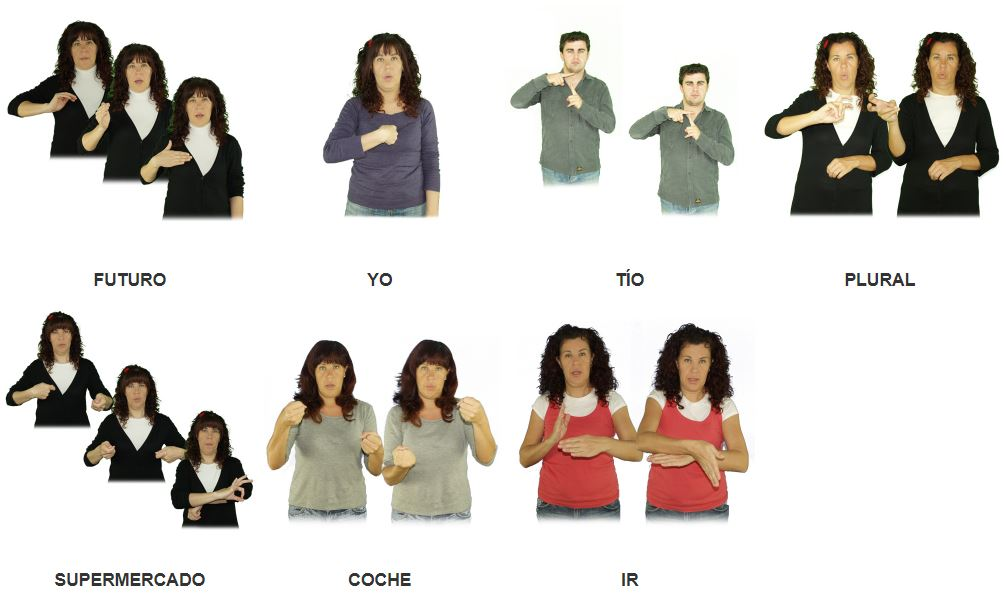
\includegraphics[width=1\textwidth]{Imagenes/Fuentes/Apendices/E17.jpg}
		\caption{Oraci�n con tiempo verbal y posesivos en LSE }
		\label {fig: AP_E17_cap8}
	\end{figure}
	
	\item \textbf{G�nero y N�mero}: Detecta el g�nero y n�mero de cada sustantivo e indica el signo de ``PLURAL'' en caso del n�mero o ``FEMENINO'' en caso del g�nero, como se puede ver en la Figura  ~\ref {fig: AP_E16_cap8}
	
	\begin{figure}[]
		\centering
		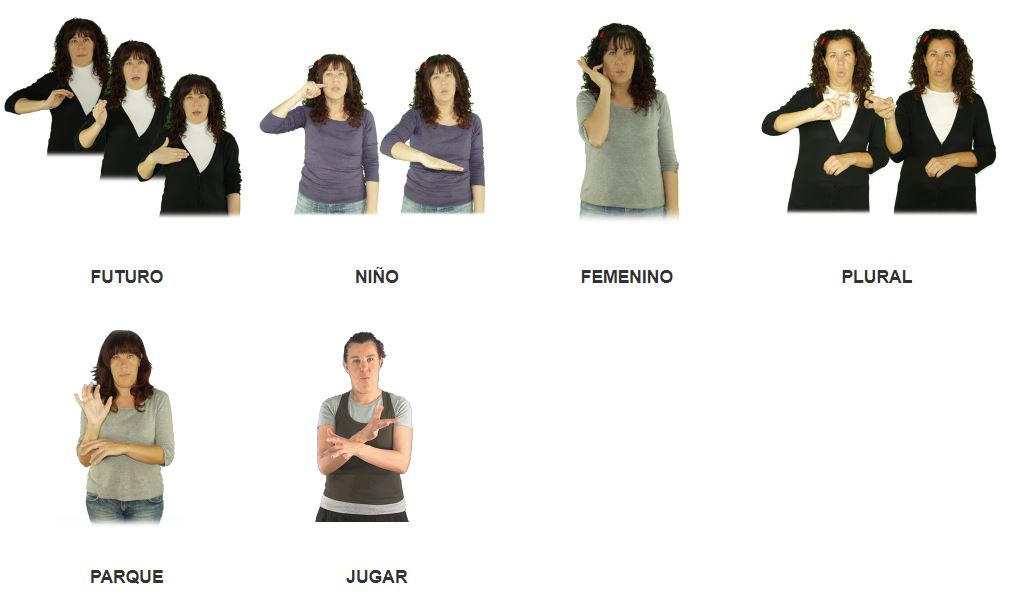
\includegraphics[width=1\textwidth]{Imagenes/Fuentes/Apendices/E16.jpg}
		\caption{Oraci�n con g�nero y n�mero en LSE }
		\label {fig: AP_E16_cap8}
	\end{figure}
	
	\item \textbf{Adjetivos}: Detecta todos los adjetivos de la oraci�n y los pasa a masculino singular como por ejemplo la Figura ~\ref {fig: AP_E2_cap8}
	
		\begin{figure}[]
		\centering
		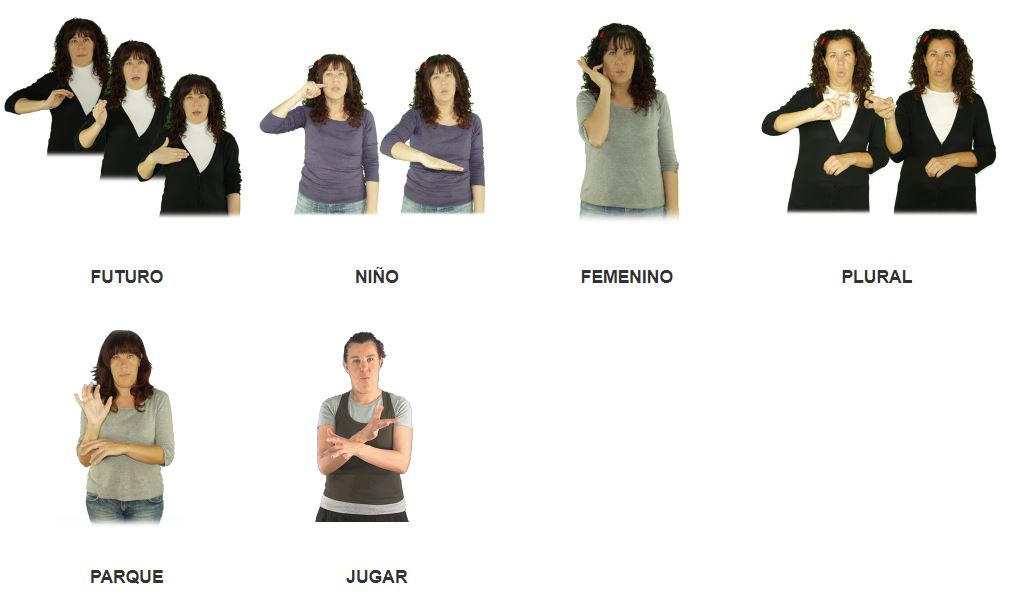
\includegraphics[width=1\textwidth]{Imagenes/Fuentes/Apendices/E16.jpg}
		\caption{Oraci�n con adjetivos en LSE }
		\label {fig: AP_E2_cap8}
	\end{figure}
	
	
\end{itemize}


Aunque queda mucho trabajo por hacer, nos gustar�a destacar que al comienzo de este TFG se hizo un an�lisis de distintas aplicaciones similares en el mercado pero no encontramos ninguna aplicaci�n que realizara traducciones de texto a LSE en tiempo real, por lo que podemos afirmar que a�n no siendo perfecto el resultado, este trabajo es una buena base para la traducci�n de lenguaje natural a Lengua de Signos Espa�ola. \\

Un objetivo tambi�n importante ha sido desarrollar una aplicaci�n mediante servicios web, de tal forma que sea f�cil de utilizar en otros proyectos o de facilitar las posibles mejoras en un futuro.\\ 


Aparte de la traducci�n, el prop�sito era crear tambi�n una aplicaci�n con una interfaz intuitiva y accesible para todos desde cualquier dispositivo. Se ten�a la intenci�n de hacer una evaluaci�n de la interfaz con usuarios reales pero debido a la Covid-19 no ha sido posible realizar dicha evaluaci�n. A�n as�, teniendo en cuenta las opiniones de los tutores en este sentido y siguiendo sus consejos de dise�o creemos que la interfaz es sencilla e intuitiva y cumplimos el objetivo marcado.\\


El desarrollo de Text2LSE nos ha permitido aplicar muchos conocimientos adquiridos durante el Grado de Ingenier�a Inform�tica en un proyecto grande y con una utilidad para la vida real, no solo para el �mbito acad�mico. Algunas asignaturas que han sido muy importantes para poder realizar este proyecto han sido:


\begin{itemize}
	
	
	\item \textbf{Aplicaciones Web: } Nos ha servido mucho a la hora de realizar el Front-end ya que nos aport� grandes conocimientos sobre el desarrollo web con HTML, CSS y Javascript que han sido muy �tiles para este TFG.
	
	\item \textbf{Tecnolog�a de la Programaci�n:} Gracias a esta asignatura aprendimos a como realizar un proyecto en JAVA. Aunque el TFG est� hecho en Python, lo importante de esta asignatura es que nos aport� un gran conocimiento a la hora de programar, por lo que aprender un nuevo lenguaje como PYTHON no ha sido tan complicado.
	
	\item \textbf{Estructura de Datos Algor�tmicos}: De esta asignatura lo que m�s nos ha ayudado ha sido saber como utilizar la recursi�n a la hora de programar, ya que ha sido un pilar fundamental en el PLN.
	
	\item \textbf{�tica, Legislaci�n y Profesi�n} Es una asignatura que nos ha ense�ado como usar las licencias con las que proteger nuestro trabajo, as� como aprender a utilizar el software libre y referenciar bien toda la informaci�n utilizada en el proyecto.
	
	
\end{itemize}

Tambi�n el proyecto nos ha permitido desarrollar muchos conocimientos nuevos que no se han cursado en la carrera, como por ejemplo: Servicios Web, Proxys, PLN, PYTHON.


\section{Trabajo Futuro}
\label{cap8:sec:TrabajoFuturo}

Con el objetivo de mejorar algunas funcionalidades de la aplicaci�n de Text2LSE de cara a obtener una aplicaci�n m�s completa, pensamos que se podr�a marcar como trabajo futuro lo siguiente:

\begin{itemize}
	

	\item \textbf{Traducci�n de nombres propios:} En la LSE los nombres propios se pueden traducir usando el signo de cada letra hasta completar el nombre, o utilizar un signo propio que defina a la persona. Actualmente la apliaci�n detecta el nombre propio pero no encuentra traducci�n, ya que no hay im�genes o v�deos para ese nombre, como se puede ver en la Figura  ~\ref {fig: AnaAlta}. La soluci�n ser�a utilizar el signo de cada letra del nombre propio como se puede ver en la Figura ~\ref {fig: NombreBien}
	
	\begin{figure}[]
		\centering
		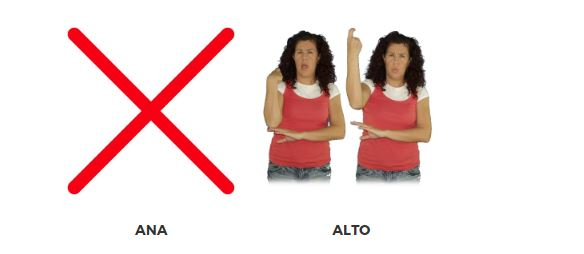
\includegraphics[width=1\textwidth]{Imagenes/Fuentes/Conclusiones/AnaAlta.jpg}
		\caption{Ejemplo de mala traducci�n de un nombre propio }
		\label {fig: AnaAlta}
	\end{figure}

	
	\begin{figure}[]
		\centering
		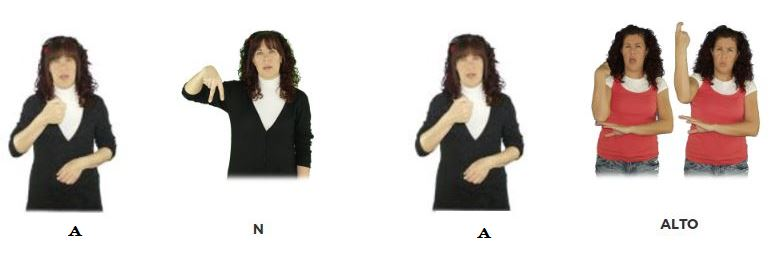
\includegraphics[width=1\textwidth]{Imagenes/Fuentes/Conclusiones/NombreBien.jpg}
		\caption{Ejemplo de buena traducci�n de un nombre propio}
		\label {fig: NombreBien}
	\end{figure}


	\item \textbf{Mejorar el G�nero y N�mero:} Como se indica en la secci�n de an�lisis de los resultados \ref{cap6:sec:An�lisis de los Resultados}, una mejora ser�a detectar cuando a�adir el signo que indica Femenino o el signo que indica el Plural, ya que hay veces que no es necesario a�adirlo, por ejemplo en la palabra ``rampas'' cuya traducci�n ser�a el signo \textit{``RAMPAS''} (Figura ~\ref {fig: rampas}). Sin embargo, la aplicaci�n a veces lo traduce como ``RAMPAS + FEMENINO + PLURAL'', como se puede ver en la Figura ~\ref {fig: rampasMal}
	
	\begin{figure}[]
		\centering
		\includegraphics[width=0.6\textwidth]{Imagenes/Fuentes/Conclusiones/rampas.jpg}
		\caption{Traducci�n correcta de la palabra rampas}
		\label {fig: rampas}
	\end{figure}

	\begin{figure}[]
		\centering
		\includegraphics[width=1\textwidth]{Imagenes/Fuentes/Conclusiones/rampasMal.jpg}
		\caption{Traducci�n incorrecta de la palabra rampas}
		\label {fig: rampasMal}
	\end{figure}

	\item \textbf{A�adir la negaci�n:} Actualmente el sistema de reglas no contempla la negaci�n de las oraciones, por lo que ser�a un gran avance a�adir una regla que permita traducir bien una oraci�n negativa en LSE, como se puede ver en la secci�n de an�lisis de los resultados \ref{cap6:sec:An�lisis de los Resultados}.

	\item \textbf{Reconocimiento de tiempos compuestos:} La aplicaci�n actualmente no es capaz de reconocer los tiempos compuestos, como pueden ser ``han comido'' o ``estaban comiendo'', por lo que ser�a importante desarrollar el PLN para que este tipo de verbos se traduzcan de manera correcta. En la Figura ~\ref {fig: hanComidoPanMal} se puede ver que intenta traducir el verbo haber y no encuentra resultado. La opci�n correcta ser�a la de la Figura ~\ref {fig: hanComidoPanBien}
	
	\begin{figure}[]
		\centering
		\includegraphics[width=1\textwidth]{Imagenes/Fuentes/Conclusiones/hanComidoPanMal.jpg}
		\caption{Ejemplo de mala traducci�n de tiempos compuestos }
		\label {fig: hanComidoPanMal}
	\end{figure}

	\begin{figure}[]
		\centering
		\includegraphics[width=1\textwidth]{Imagenes/Fuentes/Conclusiones/hanComidoPanBien.jpg}
		\caption{Ejemplo de buena traducci�n de tiempos compuestos }
		\label {fig: hanComidoPanBien}
	\end{figure}
	
	\item \textbf{Particularidad:} Contemplar frases hechas que no requieren traducci�n, ya que la LSE tiene un signo propio para esa frase. Por ejemplo la frase ``Secar el pelo'' se traduce con un solo signo, como se puede ver en la Figura ~\ref {fig: pelosecar}. Sin embargo, nuestra aplicaci�n realiza la traducci�n como si fuera una oraci�n normal. 
	
	\begin{figure}[]
		\centering
		\includegraphics[width=0.4\textwidth]{Imagenes/Fuentes/Conclusiones/pelosecar.jpg}
		\caption{Ejemplo de Particularidad }
		\label {fig: pelosecar}
	\end{figure}

	\item \textbf{Traducci�n de oraciones compuestas:} La traducci�n actual permite traducir frases simples, pero no traduce frases compuestas, como por ejemplo ``Los ni�os fueron al parque para jugar con sus amigos''. En esta oraci�n se puede apreciar que hay dos oraciones m�s simples bien distinguidas: ``Los ni�os fueron al parque'' y ``(Los ni�os) jugar con sus amigos''. Una posible mejora ser�a realizar un conjunto de reglas que permitan traducir estas frases compuestas.


	\item \textbf{Mejora en el Procesamiento de Lenguaje Natural:} El PLN utilizado en el proyecto ha sido mediante un sistema de reglas utilizando la herramienta Spacy. Este sistema no es capaz de traducir frases que no est�n contempladas en las reglas previamente programadas. Un cambio interesante y muy importante ser�a cambiar el sistema basado en reglas por uno basado en aprendizaje autom�tico, que sea capaz de aprender por s� mismo a traducir cualquier tipo de frase a base de entrenamiento.

	
\end{itemize}








%-------------------------------------------------------------------




%---------------------------------------------------------------------
%
%                          Conclusiones y Trabajo futuro Ingl�s
%
%---------------------------------------------------------------------
\begin{otherlanguage}{english}
	
\setcounter{chapter}{7}
\chapter{Conclusions and Future Work}


%-------------------------------------------------------------------

In this chapter, the final conclusions of the project are presented as well as possible improvements that could be applied as future work dhould the project continue.

\section{Conclusions}

In today's society, communication is essential in people daily life, since it allows for conveying information and exchanging opinions and feelings with each other, which is something that is essential as human beings. Nowadays, society is not completely adapted to everyone's needs, since there are many people who have different disabilities: cognitive, physical, visual, auditory... People with disabilities may sometimes feel a little isolated due to a lack of full access to information, as in the case of a person with a hearing impairment when listening to public address messages at a train station.\\

Hearing impaired people have many possibilities to communicate with others since the vast majority can read and write, but they also have a language of their own that is the Sign Language, which allows them to express emotions and feelings when communicating. In order to help hearing impaired people, we saw the need to develop a tool that would be capable of translating text into the SSL, since it could have many uses and facilitate day-to-day life to people from this group. Some of these utilities could be learning about SSL, translating film subtitles or an informative text, such as an airplane safety guide to SSL...\\

The main goal of this project is to develop an application capable of translating any text in spanish into SSL in video, image or SSL text format. Text2LSE tool  has been developed for this purpose.\\

Tex2LSE is capable of translating simple sentences structured as TIME + SUBJECT + OBJECT + VERB, in addition to taking into account a large number of grammatical rules of the SSL. Some of this rules are:



\begin{itemize}
	
	
	\item \textbf{Additional verbal tenses: }The tool detects the verbal tense of each sentence and adds the corresponding sign, either future (``FUTURO'') or past (``PASADO''), as it can be seen in Figure ~\ref {fig: AP_E15_cap8_in}.
	
	\begin{figure}[]
		\centering
		\includegraphics[width=1\textwidth]{Imagenes/Fuentes/Apendices/E15.jpg}
		\caption{Verbal tense and possessive sentence in SSL translated by Text2LSE }
		\label {fig: AP_E15_cap8_in}
	\end{figure}
	
	
	\item \textbf{Changes in possessive determinants:} The determinants that indicate possession are replaced by personal pronouns, as it can be seen in Figure ~\ref {fig: AP_E17_cap8_in}.
	
	\begin{figure}[]
		\centering
		\includegraphics[width=1\textwidth]{Imagenes/Fuentes/Apendices/E17.jpg}
		\caption{Verbal tense and possessive sentence in SSL translated by Text2LSE }
		\label {fig: AP_E17_cap8_in}
	\end{figure}
	
	\item \textbf{Gender and number}: The tool detects the gender and number of each noun and shows the signs ``PLURAL'' in the case of the number or woman (``MUJER'') in the case of gender, as it can be seen in Figure  ~\ref {fig: AP_E16_cap8_in}.
	
	\begin{figure}[]
		\centering
		\includegraphics[width=1\textwidth]{Imagenes/Fuentes/Apendices/E16.jpg}
		\caption{Sentence with gender and number in SSL translated by Text2LSE}
		\label {fig: AP_E16_cap8_in}
	\end{figure}
	
	\item \textbf{Adjectives}: It detects every adjective in the sentence and turns them to singular masculine, such as Figure ~\ref {fig: AP_E2_cap8_in}.
	
	\begin{figure}[]
		\centering
		\includegraphics[width=1\textwidth]{Imagenes/Fuentes/Apendices/E16.jpg}
		\caption{Sentence with adjectives in SSL translated by Text2LSE}
		\label {fig: AP_E2_cap8_in}
	\end{figure}
	
	
\end{itemize}

Although there is a lot of work to be done, we would like to highlight the fact that at the beginning of this project an analysis was made to similar applications on the market, but we did not find any application that carried out text translations to SSL in real time, so we can say that, though the result is not perfect, this work provides a good basis for the translation from natural language to Spanish Sign Language. \\

Another important aspect of the work that we developed was creating a public API\footnote{\url{https://holstein.fdi.ucm.es/tfg-text2lse/}} with the developed web services, in such a way that it is easy to use in other projects.\\ 

Apart from translation, the purpose was also to create an application with an intuitive interface that is accessible to everyone from any device. The initial plan was to carry out an evaluation of the interface with real users, but due to the Covid-19 crisis such an evaluation was not possible. Still, taking into account the opinions of the tutors in this regard and following their design advice, we believe that the interface is simple and intuitive and we meet the objective set.\\

The development of Text2LSE has allowed us to apply a great amount of knowledge acquired during the Computer Engineering Degree in a large project with a social utility, not only in the academic field. Some subjects that have been very important to carry out this project are:

\begin{itemize}
	
	
	\item \textbf{Web applications: } This subject helped us when doing the Front-end, since it provided us with great knowledge about web development with HTML, CSS and Javascript, which was very useful for this project.
	
	\item \textbf{Programming Technology:} Thanks to this subject we learned to program a project in Java. Although the project is programmed in Python, the important thing about this course is that it provided us with great knowledge when programming, so learning a new language like Python was not very complicated.
	
	\item \textbf{Algorithmic Data Structure}: What helped us the most in this subject was knowing how to use recursion when programming, since it has been a fundamental pillar in the NLP.
	
	\item \textbf{Ethics, Legislation and Profession}: This is a subject that taught us how to use the licenses with which to protect our work, as well as learning to use free software and to  correctly reference all the information used in the project.
	
	
\end{itemize}

Also the project allowed us to gain new knowledge that was not taught in the degree, such as: Web Services, Proxies, NLP, Python...


\section{Future Work}
\label{cap8:sec:TrabajoFuturo_in}

With the aim of improving some functionalities of the Text2LSE tool in order to obtain a more complete application and with greater coverage, we think that the following could be marked as future work:

\begin{itemize}
	
	
	\item \textbf{Proper names translation:} In the SSL, proper names can be translated using either the sign of each letter to complete the name or use a proper sign that defines the person. Currently, the application detects the proper name but cannot find a translation, since there are no images or videos for that name, as it can be seen in Figure ~\ref{fig: AnaAlta_in}. The solution would be to use the sign of each letter of the proper name, as it can be seen in Figure ~\ref{fig: NombreBien_in}
	
	\begin{figure}[]
		\centering
		\includegraphics[width=1\textwidth]{Imagenes/Fuentes/Conclusiones/AnaAlta.jpg}
		\caption{Example of bad translation of a proper name made by Text2LSE }
		\label {fig: AnaAlta_in}
	\end{figure}
	
	
	\begin{figure}[]
		\centering
		\includegraphics[width=1\textwidth]{Imagenes/Fuentes/Conclusiones/NombreBien.jpg}
		\caption{Example of a good translation of a proper name made by Text2LSE}
		\label {fig: NombreBien_in}
	\end{figure}
	
	
	\item \textbf{Improving Gender and Number:} As stated in section \ref{cap6:sec:An�lisis de los Resultados}, the detection of when to add the sings that indicate femenine or plural would be an improvement, since sometimes it is not necessary to add then, for example in the word ``rampas'' whose translation would be the sign \textit{``RAMPAS''} (Figure ~\ref {fig: rampas_in}). However, the application translates it as ``RAMPAS + FEMENINO + PLURAL'', as it can be seen in Figure ~\ref {fig: rampasMal_in}
	
	\begin{figure}[]
		\centering
		\includegraphics[width=0.6\textwidth]{Imagenes/Fuentes/Conclusiones/rampas.jpg}
		\caption{Correct translation of the word ``rampas'' by Text2LSE}
		\label {fig: rampas_in}
	\end{figure}
	
	\begin{figure}[]
		\centering
		\includegraphics[width=1\textwidth]{Imagenes/Fuentes/Conclusiones/rampasMal.jpg}
		\caption{Incorrect translation of the word ``rampas'' by Text2LSE}
		\label {fig: rampasMal_in}
	\end{figure}
	
	\item \textbf{Adding denial:} Currently, the rule system does not contemplate negative sentences, so it would be a great advance to add a rule that allows a negative sentence to be correctly translated in SSL.
	
	\item \textbf{Recognition of compound verbal tenses:} The application is currently not capable of recognizing compound tenses, such as ``han comido'' or ``estaban comiendo'', so it would be important to expand the NLP part of Text2LSE so that these types of verbs are correctly translated. In Figure ~\ref {fig: hanComidoPanMal_in} it can be seen that our application tries to translate the verb ``to have'' and finds no result. The correct option would be the one in Figure ~\ref {fig: hanComidoPanBien_in}
	
	\begin{figure}[]
		\centering
		\includegraphics[width=1\textwidth]{Imagenes/Fuentes/Conclusiones/hanComidoPanMal.jpg}
		\caption{Example of bad translation of compound times made by Text2LSE}
		\label {fig: hanComidoPanMal_in}
	\end{figure}
	
	\begin{figure}[]
		\centering
		\includegraphics[width=1\textwidth]{Imagenes/Fuentes/Conclusiones/hanComidoPanBien.jpg}
		\caption{Example of good translation of compound times made by Text2LSE}
		\label {fig: hanComidoPanBien_in}
	\end{figure}
	
	\item \textbf{Sentences that do not requiere NLP:} It contemplates the identification of sentences made that have their own sign and do not require a word-by-word translation. For example, the sentence ``Secar el pelo'' is translated with a single sign, as it can be seen in Figure ~\ref {fig: pelosecar_in}. However, our application performs the translation as if it were a normal sentence (See Figure ~\ref {fig: SecarPeloMAL_in})
	
	\begin{figure}[]
		\centering
		\includegraphics[width=0.4\textwidth]{Imagenes/Fuentes/Conclusiones/pelosecar.jpg}
		\caption{Sign in SSL for the phrase ``Secar el pelo'' }
		\label {fig: pelosecar_in}
	\end{figure}
	
	\begin{figure}[]
		\centering
		\includegraphics[width=1\textwidth]{Imagenes/Fuentes/Conclusiones/SecarPeloMAL.png}
		\caption{Sign in SSL for the phrase ``Secar el pelo'' made by Text2LSE}
		\label {fig: SecarPeloMAL_in}
	\end{figure}
	
	\item \textbf{Translation of compound sentences:} The current version of Text2LSE allows for the translation of simple sentences, but it does not translate compound sentences, such as ``Los ni�os fueron al parque para jugar con sus amigos'' In this sentence, it can be seen that there are two simpler well distinguished sentences: ``Los ni�os fueron al parque'' and ``(Los ni�os) jugar con sus amigos''. Developing a set of rules to translate compound sentences would be an improvement.
	
	
	\item \textbf{Improvement in the System NLP:} The NLP system is used in this project through a system of rules using the Spacy tool. This system is not capable of translating sentences that are not contemplated in the previously programmed rules. Changing the rule-based system to one based on machine learning, which is capable of learning by itself in order to translate any sentence would be an interesting and very important improvement.
	
	
\end{itemize}


\end{otherlanguage}





%-------------------------------------------------------------------






%\include{...}
%\include{...}
%\include{...}
%\include{...}

% Apéndices
\appendix
%---------------------------------------------------------------------
%
%                          Parte 3
%
%---------------------------------------------------------------------
%
% Parte3.tex
% Copyright 2009 Marco Antonio Gomez-Martin, Pedro Pablo Gomez-Martin
%
% This file belongs to the TeXiS manual, a LaTeX template for writting
% Thesis and other documents. The complete last TeXiS package can
% be obtained from http://gaia.fdi.ucm.es/projects/texis/
%
% Although the TeXiS template itself is distributed under the 
% conditions of the LaTeX Project Public License
% (http://www.latex-project.org/lppl.txt), the manual content
% uses the CC-BY-SA license that stays that you are free:
%
%    - to share & to copy, distribute and transmit the work
%    - to remix and to adapt the work
%
% under the following conditions:
%
%    - Attribution: you must attribute the work in the manner
%      specified by the author or licensor (but not in any way that
%      suggests that they endorse you or your use of the work).
%    - Share Alike: if you alter, transform, or build upon this
%      work, you may distribute the resulting work only under the
%      same, similar or a compatible license.
%
% The complete license is available in
% http://creativecommons.org/licenses/by-sa/3.0/legalcode
%
%---------------------------------------------------------------------

% Definici�n de la �ltima parte del manual, los ap�ndices

%\partTitle{Ap�ndices}

%\makepart

%---------------------------------------------------------------------
%
%                          Ap�ndice A
%
%---------------------------------------------------------------------

\chapter{Corpus de oraciones de instrucciones de seguridad de un vuelo}.
\label{ap1:A}
\begin{enumerate}


 \item Hola, les damos la bienvenida a este vuelo de Iberia en nuestro nombre y en el de Madrid. 
 \item Antes de despegar tenemos que darles unas instrucciones de seguridad. 
 \item Es importante que presten atenci�n. 
 \item Durante el despegue y aterrizaje. 
 \item Los dispositivos electr�nicos deber�n permanecer desenchufados y en modo avi�n. 
 \item Despu�s podr�n utilizarlos durante todo el vuelo.
 \item Excepto cuando la tripulaci�n les pida que los apaguen. 
 \item Recuerden que este avi�n dispone de conexi�n Wifi.
 \item Y que podr�n conectarse a Internet cuando se lo comuniquemos. 
 \item Si han tra�do equipaje de mano.
 \item Por favor, col�quelo en los compartimentos situados encima de sus butacas o debajo de sus asientos delanteros.
 \item Dejando despejados los pasillos y salidas de emergencia. 
 \item Durante el vuelo podr�n ponerse c�modos.
 \item Pero durante el despegue y aterrizaje.
 \item Por favor, pongan sus asientos en posici�n vertical.
 \item Y mantengan su mesa plegada. 
 \item Por su seguridad.
 \item Les recomendamos que mantengan su cintur�n abrochado y visible durante todo el vuelo. 
 \item Y siempre que la se�al luminosa lo indique. 
 \item Para abrocharlo.
 \item Inserte la trabilla en su enganche correspondiente. 
 \item Para soltarlo.
 \item Simplemente levanten la leng�eta del enganche. 
 \item Este avi�n cuenta con ocho puertas y dos ventanas de salida, 4 puertas a cada lado del avi�n y una ventana sobre cada ala. 
 \item Todas est�n se�alizadas con la palabra EXIT. 
 \item Y disponen de rampas o balsas de evacuaci�n. 
 \item Debajo de sus asientos encontrar�n un chaleco salvavidas. 
 \item S�quenlo de la bolsa.
 \item Y para pon�rselo.
 \item Introduzcan la cabeza por la abertura.
 \item Y pasen la cinta de atado por detr�s de su cintura.
 \item Enganchando la fijaci�n de la hebilla de un extremo a otro. 
 \item Y tirando de la cinta para ajust�rselo. 
 \item Para inflarlo.
 \item Solo tienen que tirar con fuerza del tirador del pl�stico rojo.
 \item O soplar por el tubo. 
 \item Y recuerden.
 \item Nunca deben inflar el chaleco dentro del avi�n. 
 \item En caso de despresurizaci�n de la cabina.
 \item Se abrir� autom�ticamente un compartimento sobre sus asientos.
 \item Que contiene m�scaras de ox�geno. 
 \item Tire de la suya.
 \item Col�quela sobre su nariz y boca.
 \item Y respire con normalidad. 
 \item Despu�s preste ayuda a qui�n pueda depender de usted. 
 \item Recuerden.
 \item Que para evitar poner en peligro la seguridad de este vuelo.
 \item No est� permitido fumar.
 \item O usar dispositivos de liberaci�n de nicotina en ning�n caso. 
 \item Y no olviden.
 \item Que tienen m�s informaci�n en las instrucciones de seguridad.
 \item Que encontrar�n en la bolsa delantera de sus asientos. 
 \item Muchas gracias por su atenci�n. 
 \item Esperamos que disfruten de un feliz vuelo.
 
\end{enumerate}


  
%---------------------------------------------------------------------
%
%                          Ap�ndice B
%
%---------------------------------------------------------------------

\chapter{Corpus de oraciones de un cap�tulo de una serie infantil}
\label{ap1:B}
\begin{enumerate}


 \item Yo soy Pepa.
 \item Este es mi hermano peque�o. 
 \item Esta es mam� Pig. 
 \item Este es pap� Pig. 
 \item Hoy est� lloviendo. 
 \item As� que Pepa no puede jugar fuera.
 \item Ha dejado de llover. 
 \item �Podemos salir a jugar?
 \item Salid un rato. 
 \item A Pepa le encanta saltar en los charcos.
 \item Me encanta saltar en los charcos.
 \item Si vas a pisar charcos debes ponerte las botas de agua. 
 \item Lo siento.
 \item A George tambi�n le gusta saltar en los charcos.
 \item Si vas a saltar en los charcos, debes ponerte tus botas.
 \item A Pepa le gusta cuidar de su hermano peque�o. 
 \item Vamos a buscar m�s charcos.
 \item Pepa y George se lo est�n pasando muy bien. 
 \item Pepa ha encontrado un charco peque�o. 
 \item Ese charco s� que es grande.
 \item George quiere ser el primero en saltar en el gran charco. 
 \item Tengo que ver si es seguro para ti.
 \item Parece seguro para t�. 
 \item Solo es barro. 
 \item Vamos a ense�arselo a Papi. 
 \item Adivina qu� hemos estado haciendo. 
 \item D�jame pensar. 
 \item Hab�is estado saltando en los charcos de barro.
 \item Hemos saltado en los charcos de barro.
 \item Mirad c�mo os hab�is puesto.
 \item No pasa nada.
 \item S�lo es barro. 
 \item Voy a limpiaros antes de que os vea mam�. 
 \item Podemos jugar todos juntos.
 \item Pepa y George llevan sus botas de agua.

\end{enumerate}


  
%---------------------------------------------------------------------
%
%                          Ap�ndice C
%
%---------------------------------------------------------------------

\chapter{Corpus de subt�tulos de un trailer de una pel�cula}
\label{ap1:C}
\begin{enumerate}


 \item Mi negocio son los perros.
 \item El coraz�n de un superviviente. 
 \item Le gan� a todos los dem�s. 
 \item �l no es un perro de trineo.
 \item Es un ganador. 
 \item Lo que tienen nuestros ni�os no es una epidemia, es una sentencia de muerte. 
 \item Encontraron la cura.
 \item Solo un hombre y un perro pueden hacer esa carrera. 
 \item Tiene 12 a�os.
 \item Es demasiado viejo.
 \item Pienso que no los vamos a poder encontrar despu�s de deshielo. 
 \item Es el momento de descubrir quienes somos.
 \item Yo siempre pens� que viv�a para los trineos.


\end{enumerate}


  
%---------------------------------------------------------------------
%
%                          Ap�ndice D
%
%---------------------------------------------------------------------

\chapter{Corpus de subt�tulos de un anuncio}
\label{ap1:D}
\begin{enumerate}


 \item Qu�date en casa.
 \item Mant�n una distancia de dos metros. 
 \item No te toques la cara. 
 \item L�vate las manos con frecuencia. 
 \item Evita tocar cualquier superficie si es necesario. 
 \item No saludes dando la mano.
 \item No des besos ni abrazos. 
 \item Puedes saludar con la mirada o de palabra.
 \item Mant�n tu tel�fono m�vil limpio. 
 \item Si tienes s�ntomas.
 \item Qu�date en casa y a�slate en tu habitaci�n.
 

\end{enumerate}


  
%---------------------------------------------------------------------
%
%                          Ap�ndice B
%
%---------------------------------------------------------------------

\chapter{Corpus de frases simples}
\label{ap1:E}
\begin{enumerate}


 \item �l bebe agua.
 \item Yo soy morena. 
 \item Ellos parecen contentos. 
 \item Mar�a compra galletas. 
 \item Yo bebo agua. 
 \item Yo como carne.
 \item Ellos compraron aceite. 
 \item �l vender� refrescos
 \item Ella gan� la carrera. 
 \item Yo har� la cama.
 \item Mi t�a y mi hermana beber�n agua
 \item Ella y �l comieron arroz. 
 \item Mar�a y Javier nadan.
 \item Mi hermana y mi t�a est�n de vacaciones en la playa.
 \item Los ni�os comer�n chocolate negro.
 \item Las ni�as jugar�n en el parque. 
 \item Mis t�os ir�n al supermercado en coche.
 \item Los ni�os jugar�n con la pelota. 
 \item Los ganadores recibir�n un trofeo de oro. 
 \item �l pasa ante la casa todos los d�as.
 \item �l pasea ante la casa por la ma�ana
 \item Ma�ana yo ir� al m�dico.
 \item �l comi� mucho en la fiesta. 
 \item �l se comi� la hamburguesa aqu�. 
 \item Mi t�a conduce muy despacio. 


\end{enumerate}


  
%---------------------------------------------------------------------
%
%                          Ap�ndice A
%
%---------------------------------------------------------------------
\chapter{Traducci�n de los corpus mediante Text2LSE}.
\label{ap1:F}
%-------------------------------------------------------------------
\section{Corpus de oraciones de instrucciones de seguridad de un vuelo}
%-------------------------------------------------------------------
\label{ap1:F_A}

\begin{enumerate}
  \item Hola, les damos la bienvenida a este vuelo de Iberia en nuestro nombre y en el de Madrid. 
 \begin{figure}[H]
 	\centering
 	\includegraphics[width=1\textwidth]{Imagenes/Fuentes/apendices/A1_1.jpg}
 	\label {fig: AP_A1.1}
 \end{figure}
\begin{figure}[H]
	\centering
	\includegraphics[width=1\textwidth]{Imagenes/Fuentes/apendices/A1_2.jpg}
	\label {fig: AP_A1.2}
\end{figure}
\begin{figure}[H]
	\centering
	\includegraphics[width=0.6\textwidth]{Imagenes/Fuentes/apendices/A1_3.jpg}
	\label {fig: AP_A1.3}
\end{figure}
 
 \item Antes de despegar tenemos que darles unas instrucciones de seguridad. 
 
 \begin{figure}[H]
 	\centering
 	\includegraphics[width=1\textwidth]{Imagenes/Fuentes/apendices/A2.jpg}
 	\label {fig: AP_A2}
 \end{figure}
 
 \item Es importante que presten atenci�n. 
 
 \begin{figure}[H]
 	\centering
 	\includegraphics[width=1\textwidth]{Imagenes/Fuentes/apendices/A3.jpg}
 	\label {fig: AP_A3}
 \end{figure}
 
 \item Durante el despegue y aterrizaje. 
 
 \begin{figure}[H]
 	\centering
 	\includegraphics[width=1\textwidth]{Imagenes/Fuentes/apendices/A4.jpg}
 	\label {fig: AP_A4}
 \end{figure}
 
 \item Los dispositivos electr�nicos deber�n permanecer desenchufados y en modo avi�n. 
 
 \begin{figure}[H]
 	\centering
 	\includegraphics[width=1\textwidth]{Imagenes/Fuentes/apendices/A5.jpg}
 	\label {fig: AP_A5}
 \end{figure}

\newpage
 \item Despu�s podr�n utilizarlos durante todo el vuelo.
 
 \begin{figure}[H]
 	\centering
 	\includegraphics[width=1\textwidth]{Imagenes/Fuentes/apendices/A6.jpg}
 	\label {fig: AP_A6}
 \end{figure}
 
 \item Excepto cuando la tripulaci�n les pida que los apaguen. 
 
 \begin{figure}[H]
 	\centering
 	\includegraphics[width=1\textwidth]{Imagenes/Fuentes/apendices/A7.jpg}
 	\label {fig: AP_A7}
 \end{figure}

\newpage
 \item Recuerden que este avi�n dispone de conexi�n Wifi.
 
 \begin{figure}[H]
 	\centering
 	\includegraphics[width=1\textwidth]{Imagenes/Fuentes/apendices/A8.jpg}
 	\label {fig: AP_A8}
 \end{figure}

 \item Y que podr�n conectarse a Internet cuando se lo comuniquemos. 
 
 \begin{figure}[H]
 	\centering
 	\includegraphics[width=1\textwidth]{Imagenes/Fuentes/apendices/A9.jpg}
 	\label {fig: AP_A9}
 \end{figure}
 \newpage
 \item Si han tra�do equipaje de mano.
 
  \begin{figure}[H]
 	\centering
 	\includegraphics[width=1\textwidth]{Imagenes/Fuentes/apendices/A10.jpg}
 	\label {fig: AP_A10}
 \end{figure}
 
 \item Por favor, col�quelo en los compartimentos situados encima de sus butacas o debajo de sus asientos delanteros.
 
\begin{figure}[H]
	\centering
	\includegraphics[width=1\textwidth]{Imagenes/Fuentes/apendices/A11_1.jpg}
	\label {fig: AP_A11_1}
\end{figure}

\begin{figure}[H]
	\centering
	\includegraphics[width=1\textwidth]{Imagenes/Fuentes/apendices/A11_2.jpg}
	\label {fig: AP_A11_2}
\end{figure}

 \item Dejando despejados los pasillos y salidas de emergencia. 
 
   \begin{figure}[H]
 	\centering
 	\includegraphics[width=1\textwidth]{Imagenes/Fuentes/apendices/A12.jpg}
 	\label {fig: AP_A12}
 \end{figure}
 
   \newpage
 \item Durante el vuelo podr�n ponerse c�modos.
 

\begin{figure}[H]
 	\centering
 	\includegraphics[width=1\textwidth]{Imagenes/Fuentes/apendices/A13.jpg}
 	\label {fig: AP_A13}
 \end{figure}

 \item Pero durante el despegue y aterrizaje.
 
 \begin{figure}[H]
 	\centering
 	\includegraphics[width=1\textwidth]{Imagenes/Fuentes/apendices/A14.jpg}
 	\label {fig: AP_A14}
 \end{figure}
 
   \newpage
 \item Por favor, pongan sus asientos en posici�n vertical.
 
  \begin{figure}[H]
 	\centering
 	\includegraphics[width=1\textwidth]{Imagenes/Fuentes/apendices/A15.jpg}
 	\label {fig: AP_A15}
 \end{figure}
 
 \item Y mantengan su mesa plegada.
 
  \begin{figure}[H]
 	\centering
 	\includegraphics[width=1\textwidth]{Imagenes/Fuentes/apendices/A16.jpg}
 	\label {fig: AP_A16}
 \end{figure}

  \newpage
 \item Por su seguridad.
 
 \begin{figure}[H]
 	\centering
 	\includegraphics[width=1\textwidth]{Imagenes/Fuentes/apendices/A17.jpg}
 	\label {fig: AP_A17}
 \end{figure}
 
 \item Les recomendamos que mantengan su cintur�n abrochado y visible durante todo el vuelo.
 
  \begin{figure}[H]
 	\centering
 	\includegraphics[width=1\textwidth]{Imagenes/Fuentes/apendices/A18.jpg}
 	\label {fig: AP_A18}
 \end{figure}
  \newpage
  
 \item Y siempre que la se�al luminosa lo indique.
 
 \begin{figure}[H]
 	\centering
 	\includegraphics[width=1\textwidth]{Imagenes/Fuentes/apendices/A19.jpg}
 	\label {fig: AP_A19}
 \end{figure}
  
 \item Para abrocharlo.
 
\begin{figure}[H]
	\centering
	\includegraphics[width=0.6\textwidth]{Imagenes/Fuentes/apendices/A20.jpg}
	\label {fig: AP_A20}
\end{figure}
 
 \newpage
 \item Inserte la trabilla en su enganche correspondiente. 
 
\begin{figure}[H]
	\centering
	\includegraphics[width=1\textwidth]{Imagenes/Fuentes/apendices/A21.jpg}
	\label {fig: AP_A21}
\end{figure}

 \item Para soltarlo.
 
\begin{figure}[H]
	\centering
	\includegraphics[width=0.6\textwidth]{Imagenes/Fuentes/apendices/A22.jpg}
	\label {fig: AP_A22}
\end{figure}
 
 \item Simplemente levanten la leng�eta del enganche.
 
 \begin{figure}[H]
	\centering
	\includegraphics[width=1\textwidth]{Imagenes/Fuentes/apendices/A23.jpg}
	\label {fig: AP_A23}
\end{figure}
  \newpage
 \item Este avi�n cuenta con ocho puertas y dos ventanas de salida, 4 puertas a cada lado del avi�n y una ventana sobre cada ala. 
 
\begin{figure}[H]
	\centering
	\includegraphics[width=1\textwidth]{Imagenes/Fuentes/apendices/A24_1.jpg}
	\label {fig: AP_A24_1}
\end{figure}

\begin{figure}[H]
	\centering
	\includegraphics[width=1\textwidth]{Imagenes/Fuentes/apendices/A24_2.jpg}
	\label {fig: AP_A24_2}
\end{figure}

\begin{figure}[H]
	\centering
	\includegraphics[width=1\textwidth]{Imagenes/Fuentes/apendices/A24_3.jpg}
	\label {fig: AP_A24_3}
\end{figure}

\begin{figure}[H]
	\centering
	\includegraphics[width=1\textwidth]{Imagenes/Fuentes/apendices/A24_4.jpg}
	\label {fig: AP_A24_4}
\end{figure}
  \newpage
 \item Todas est�n se�alizadas con la palabra EXIT.

 \begin{figure}[H]
 	\centering
 	\includegraphics[width=1\textwidth]{Imagenes/Fuentes/apendices/A25.jpg}
 	\label {fig: AP_A25}
 \end{figure}
  
 \item Y disponen de rampas o balsas de evacuaci�n. 
 
  \begin{figure}[H]
 	\centering
 	\includegraphics[width=1\textwidth]{Imagenes/Fuentes/apendices/A26.jpg}
 	\label {fig: AP_A26}
 \end{figure}

\newpage
 \item Debajo de sus asientos encontrar�n un chaleco salvavidas. 
 
 \begin{figure}[H]
 	\centering
 	\includegraphics[width=1\textwidth]{Imagenes/Fuentes/apendices/A27.jpg}
 	\label {fig: AP_A27}
 \end{figure}
 
   
 \item S�quenlo de la bolsa.
 
  \begin{figure}[H]
 	\centering
 	\includegraphics[width=0.6\textwidth]{Imagenes/Fuentes/apendices/A28.jpg}
 	\label {fig: AP_A28}
 \end{figure}
 
 \newpage
 \item Y para pon�rselo.
 
\begin{figure}[H]
	\centering
	\includegraphics[width=0.6\textwidth]{Imagenes/Fuentes/apendices/A29.jpg}
	\label {fig: AP_A29}
\end{figure}
 

 \item Introduzcan la cabeza por la abertura.
 
 \begin{figure}[H]
 	\centering
 	\includegraphics[width=1\textwidth]{Imagenes/Fuentes/apendices/A30.jpg}
 	\label {fig: AP_A30}
 \end{figure}
 
 \newpage
 \item Y pasen la cinta de atado por detr�s de su cintura.
 
\begin{figure}[H]
	\centering
	\includegraphics[width=1\textwidth]{Imagenes/Fuentes/apendices/A31.jpg}
	\label {fig: AP_A31}
\end{figure}
 
 \item Enganchando la fijaci�n de la hebilla de un extremo a otro. 
 
 \begin{figure}[H]
 	\centering
 	\includegraphics[width=1\textwidth]{Imagenes/Fuentes/apendices/A32.jpg}
 	\label {fig: AP_A32}
 \end{figure}
 \newpage

 \item Y tirando de la cinta para ajust�rselo.
 
\begin{figure}[H]
	\centering
	\includegraphics[width=1\textwidth]{Imagenes/Fuentes/apendices/A33.jpg}
	\label {fig: AP_A33}
\end{figure}


 \item Para inflarlo.
 
 \begin{figure}[H]
 	\centering
 	\includegraphics[width=0.6\textwidth]{Imagenes/Fuentes/apendices/A34.jpg}
 	\label {fig: AP_A34}
 \end{figure}

\newpage
 \item Solo tienen que tirar con fuerza del tirador del pl�stico rojo.
 
\begin{figure}[H]
	\centering
	\includegraphics[width=1\textwidth]{Imagenes/Fuentes/apendices/A35.jpg}
	\label {fig: AP_A35}
\end{figure}

  
 \item O soplar por el tubo. 
 
\begin{figure}[H]
	\centering
	\includegraphics[width=1\textwidth]{Imagenes/Fuentes/apendices/A36.jpg}
	\label {fig: AP_A36}
\end{figure}
 
\newpage
 \item Y recuerden.
 
\begin{figure}[H]
	\centering
	\includegraphics[width=0.4\textwidth]{Imagenes/Fuentes/apendices/A37.jpg}
	\label {fig: AP_A37}
\end{figure}
 
 \item Nunca deben inflar el chaleco dentro del avi�n. 
 
\begin{figure}[H]
\centering
\includegraphics[width=1\textwidth]{Imagenes/Fuentes/apendices/A38.jpg}
\label {fig: AP_A38}
\end{figure}
 
   \newpage
 \item En caso de despresurizaci�n de la cabina.
 
\begin{figure}[H]
	\centering
	\includegraphics[width=1\textwidth]{Imagenes/Fuentes/apendices/A39.jpg}
	\label {fig: AP_A39}
\end{figure}
 
 \item Se abrir� autom�ticamente un compartimento sobre sus asientos.
 
\begin{figure}[H]
	\centering
	\includegraphics[width=1\textwidth]{Imagenes/Fuentes/apendices/A40.jpg}
	\label {fig: AP_A40}
\end{figure}

  \newpage
 \item Que contiene m�scaras de ox�geno. 
 
 \begin{figure}[H]
 	\centering
 	\includegraphics[width=1\textwidth]{Imagenes/Fuentes/apendices/A41.jpg}
 	\label {fig: AP_A41}
 \end{figure}

 \item Tire de la suya.
 
  \begin{figure}[H]
 	\centering
 	\includegraphics[width=0.6\textwidth]{Imagenes/Fuentes/apendices/A42.jpg}
 	\label {fig: AP_A42}
 \end{figure}
 
   \newpage
 \item Col�quela sobre su nariz y boca.
 
\begin{figure}[H]
	\centering
	\includegraphics[width=1\textwidth]{Imagenes/Fuentes/apendices/A43.jpg}
	\label {fig: AP_A43}
\end{figure}


 \item Y respire con normalidad. 
 
 \begin{figure}[H]
 	\centering
 	\includegraphics[width=1\textwidth]{Imagenes/Fuentes/apendices/A44.jpg}
 	\label {fig: AP_A44}
 \end{figure}
 
   \newpage
 \item Despu�s preste ayuda a qui�n pueda depender de usted. 
 
 \begin{figure}[H]
	\centering
	\includegraphics[width=1\textwidth]{Imagenes/Fuentes/apendices/A45.jpg}
	\label {fig: AP_A45}
\end{figure}

 \item Recuerden.
 
  \begin{figure}[H]
 	\centering
 	\includegraphics[width=0.3\textwidth]{Imagenes/Fuentes/apendices/A46.jpg}
 	\label {fig: AP_A46}
 \end{figure}
 
   \newpage
 \item Que para evitar poner en peligro la seguridad de este vuelo.
 
  \begin{figure}[H]
 	\centering
 	\includegraphics[width=1\textwidth]{Imagenes/Fuentes/apendices/A47.jpg}
 	\label {fig: AP_A47}
 \end{figure}
 

 \item No est� permitido fumar.
 
\begin{figure}[H]
	\centering
	\includegraphics[width=1\textwidth]{Imagenes/Fuentes/apendices/A48.jpg}
	\label {fig: AP_A48}
\end{figure}
 
   \newpage
 \item O usar dispositivos de liberaci�n de nicotina en ning�n caso. 
 
 \begin{figure}[H]
 	\centering
 	\includegraphics[width=1\textwidth]{Imagenes/Fuentes/apendices/A49.jpg}
 	\label {fig: AP_A49}
 \end{figure}
 
 
 \item Y no olviden.
 
  \begin{figure}[H]
 	\centering
 	\includegraphics[width=0.6\textwidth]{Imagenes/Fuentes/apendices/A50.jpg}
 	\label {fig: AP_A50}
 \end{figure}
 
   \newpage
 \item Que tienen m�s informaci�n en las instrucciones de seguridad.
 
\begin{figure}[H]
	\centering
	\includegraphics[width=1\textwidth]{Imagenes/Fuentes/apendices/A51.jpg}
	\label {fig: AP_A51}
\end{figure}

 \item Que encontrar�n en la bolsa delantera de sus asientos. 
 
 \begin{figure}[H]
 	\centering
 	\includegraphics[width=1\textwidth]{Imagenes/Fuentes/apendices/A52.jpg}
 	\label {fig: AP_A52}
 \end{figure}

   \newpage
 \item Muchas gracias por su atenci�n. 
 
\begin{figure}[H]
	\centering
	\includegraphics[width=1\textwidth]{Imagenes/Fuentes/apendices/A53.jpg}
	\label {fig: AP_A53}
\end{figure}
 
 \item Esperamos que disfruten de un feliz vuelo.
 
 \begin{figure}[H]
 	\centering
 	\includegraphics[width=1\textwidth]{Imagenes/Fuentes/apendices/A54.jpg}
 	\label {fig: AP_A54}
 \end{figure}
 
\end{enumerate}

\newpage
  %-------------------------------------------------------------------
  \section{Corpus de oraciones de un cap�tulo de una serie infantil}
  %-------------------------------------------------------------------
  \label{ap1:F_B}
  
  \begin{enumerate}
  	
  	
  	\item Yo soy Pepa.
  	
  	 \begin{figure}[H]
  		\centering
  		\includegraphics[width=0.6\textwidth]{Imagenes/Fuentes/apendices/B1.jpg}
  		\label {fig: AP_B1}
  	\end{figure}
  
  	\item Este es mi hermano peque�o.
  	
  	 \begin{figure}[H]
  		\centering
  		\includegraphics[width=1\textwidth]{Imagenes/Fuentes/apendices/B2.jpg}
  		\label {fig: AP_B2}
  	\end{figure}
  	 \newpage
  	\item Esta es mam� Pig. 
  	
  	\begin{figure}[H]
  		\centering
  		\includegraphics[width=1\textwidth]{Imagenes/Fuentes/apendices/B3.jpg}
  		\label {fig: AP_B3}
  	\end{figure}
  	
  	\item Este es pap� Pig. 
  	
	\begin{figure}[H]
		\centering
		\includegraphics[width=1\textwidth]{Imagenes/Fuentes/apendices/B4.jpg}
		\label {fig: AP_B4}
	\end{figure}
  	
  	 \newpage
  	\item Hoy est� lloviendo. 
  	
  	\begin{figure}[H]
  		\centering
  		\includegraphics[width=1\textwidth]{Imagenes/Fuentes/apendices/B5.jpg}
  		\label {fig: AP_B5}
  	\end{figure}
  	
  	\item As� que Pepa no puede jugar fuera.
  	
  	\begin{figure}[H]
  		\centering
  		\includegraphics[width=1\textwidth]{Imagenes/Fuentes/apendices/B6.jpg}
  		\label {fig: AP_B6}
  	\end{figure}
  	
  	 \newpage
  	\item Ha dejado de llover. 
  	
  	\begin{figure}[H]
  		\centering
  		\includegraphics[width=1\textwidth]{Imagenes/Fuentes/apendices/B7.jpg}
  		\label {fig: AP_B7}
  	\end{figure}
  	
  	\item �Podemos salir a jugar?
  	
  	\begin{figure}[H]
  		\centering
  		\includegraphics[width=1\textwidth]{Imagenes/Fuentes/apendices/B8.jpg}
  		\label {fig: AP_B8}
  	\end{figure}
  	
  	 \newpage
  	\item Salid un rato. 
  	
  	\begin{figure}[H]
  		\centering
  		\includegraphics[width=1\textwidth]{Imagenes/Fuentes/apendices/B9.jpg}
  		\label {fig: AP_B9}
  	\end{figure}
  	
  	\item A Pepa le encanta saltar en los charcos.
  	
  	\begin{figure}[H]
  		\centering
  		\includegraphics[width=1\textwidth]{Imagenes/Fuentes/apendices/B10.jpg}
  		\label {fig: AP_B10}
  	\end{figure}
  	
  	\item Me encanta saltar en los charcos.
  	
  	\begin{figure}[H]
  		\centering
  		\includegraphics[width=1\textwidth]{Imagenes/Fuentes/apendices/B11.jpg}
  		\label {fig: AP_B11}
  	\end{figure}
  	
  	 \newpage
  	\item Si vas a pisar charcos debes ponerte las botas de agua. 
  	
  	\begin{figure}[H]
  		\centering
  		\includegraphics[width=1\textwidth]{Imagenes/Fuentes/apendices/B12.jpg}
  		\label {fig: AP_B12}
  	\end{figure}
  	
  	\item Lo siento.
  	
  	\begin{figure}[H]
  		\centering
  		\includegraphics[width=0.3\textwidth]{Imagenes/Fuentes/apendices/B13.jpg}
  		\label {fig: AP_B13}
  	\end{figure}
  	\newpage
  	\item A George tambi�n le gusta saltar en los charcos.
  	
  	\begin{figure}[H]
  		\centering
  		\includegraphics[width=1\textwidth]{Imagenes/Fuentes/apendices/B14.jpg}
  		\label {fig: AP_B14}
  	\end{figure}
  	
  	\item Si vas a saltar en los charcos, debes ponerte tus botas.
  	
  	\begin{figure}[H]
  		\centering
  		\includegraphics[width=1\textwidth]{Imagenes/Fuentes/apendices/B15.jpg}
  		\label {fig: AP_B15}
  	\end{figure}
  
  	\newpage
  	\item A Pepa le gusta cuidar de su hermano peque�o. 
  	
  	\begin{figure}[H]
  		\centering
  		\includegraphics[width=1\textwidth]{Imagenes/Fuentes/apendices/B16.jpg}
  		\label {fig: AP_B16}
  	\end{figure}
  	
  	\item Vamos a buscar m�s charcos.
  	
  	\begin{figure}[H]
  		\centering
  		\includegraphics[width=1\textwidth]{Imagenes/Fuentes/apendices/B17.jpg}
  		\label {fig: AP_B17}
  	\end{figure}
  	
  	\newpage
  	\item Pepa y George se lo est�n pasando muy bien. 
  	
  	\begin{figure}[H]
  		\centering
  		\includegraphics[width=1\textwidth]{Imagenes/Fuentes/apendices/B18.jpg}
  		\label {fig: AP_B18}
  	\end{figure}
  	
  	\item Pepa ha encontrado un charco peque�o. 
  	
  	\begin{figure}[H]
  		\centering
  		\includegraphics[width=1\textwidth]{Imagenes/Fuentes/apendices/B19.jpg}
  		\label {fig: AP_B19}
  	\end{figure}
  	
  	\newpage
  	\item Ese charco s� que es grande.
  	
  	\begin{figure}[H]
  		\centering
  		\includegraphics[width=1\textwidth]{Imagenes/Fuentes/apendices/B20.jpg}
  		\label {fig: AP_B20}
  	\end{figure}
  	
  	\item George quiere ser el primero en saltar en el gran charco. 
  	
  	\begin{figure}[H]
  		\centering
  		\includegraphics[width=1\textwidth]{Imagenes/Fuentes/apendices/B21.jpg}
  		\label {fig: AP_B21}
  	\end{figure}
  	
  	\newpage
  	\item Tengo que ver si es seguro para ti.
  	
  	\begin{figure}[H]
  		\centering
  		\includegraphics[width=1\textwidth]{Imagenes/Fuentes/apendices/B22.jpg}
  		\label {fig: AP_B22}
  	\end{figure}
  	
  	\item Parece seguro para t�. 
  	
  	\begin{figure}[H]
  		\centering
  		\includegraphics[width=1\textwidth]{Imagenes/Fuentes/apendices/B23.jpg}
  		\label {fig: AP_B23}
  	\end{figure}
  	\newpage
  	\item Solo es barro. 
  	
  	\begin{figure}[H]
  		\centering
  		\includegraphics[width=0.6\textwidth]{Imagenes/Fuentes/apendices/B24.jpg}
  		\label {fig: AP_B24}
  	\end{figure}
  	
  	
  	\item Vamos a ense�arselo a Papi. 
  	
  	\begin{figure}[H]
  		\centering
  		\includegraphics[width=1\textwidth]{Imagenes/Fuentes/apendices/B25.jpg}
  		\label {fig: AP_B25}
  	\end{figure}
  	
  	\item Adivina qu� hemos estado haciendo. 
  	
  	\begin{figure}[H]
  		\centering
  		\includegraphics[width=1\textwidth]{Imagenes/Fuentes/apendices/B26.jpg}
  		\label {fig: AP_B26}
  	\end{figure}
  	
  	\newpage
  	\item D�jame pensar. 
  	
  	\begin{figure}[H]
  		\centering
  		\includegraphics[width=0.3\textwidth]{Imagenes/Fuentes/apendices/B27.jpg}
  		\label {fig: AP_B27}
  	\end{figure}
  	
  	\item Hab�is estado saltando en los charcos de barro.
  	
  	\begin{figure}[H]
  		\centering
  		\includegraphics[width=1\textwidth]{Imagenes/Fuentes/apendices/B28.jpg}
  		\label {fig: AP_B28}
  	\end{figure}
  	
  	\newpage
  	\item Hemos saltado en los charcos de barro.
  	
 	\begin{figure}[H]
  		\centering
  		\includegraphics[width=1\textwidth]{Imagenes/Fuentes/apendices/B29.jpg}
  		\label {fig: AP_B29}
  	\end{figure}
  	
  	\item Mirad c�mo os hab�is puesto.
  	
 	\begin{figure}[H]
  		\centering
  		\includegraphics[width=1\textwidth]{Imagenes/Fuentes/apendices/B30.jpg}
  		\label {fig: AP_B30}
  	\end{figure}
  	
  	\newpage
  	\item No pasa nada.
  	
  	\begin{figure}[H]
  		\centering
  		\includegraphics[width=1\textwidth]{Imagenes/Fuentes/apendices/B31.jpg}
  		\label {fig: AP_B31}
  	\end{figure}
  	
  	\item S�lo es barro. 
  	
  	\begin{figure}[H]
  		\centering
  		\includegraphics[width=0.6\textwidth]{Imagenes/Fuentes/apendices/B32.jpg}
  		\label {fig: AP_B32}
  	\end{figure}
  	
  	\newpage
  	\item Voy a limpiaros antes de que os vea mam�. 
  	
  	\begin{figure}[H]
  		\centering
  		\includegraphics[width=1\textwidth]{Imagenes/Fuentes/apendices/B33.jpg}
  		\label {fig: AP_B33}
  	\end{figure}
  	
  	\item Podemos jugar todos juntos.
  	
  	\begin{figure}[H]
  		\centering
  		\includegraphics[width=1\textwidth]{Imagenes/Fuentes/apendices/B34.jpg}
  		\label {fig: AP_B34}
  	\end{figure}
  	
  	\newpage
  	\item Pepa y George llevan sus botas de agua.
  	
 	\begin{figure}[H]
  		\centering
  		\includegraphics[width=1\textwidth]{Imagenes/Fuentes/apendices/B35.jpg}
  		\label {fig: AP_B35}
  	\end{figure}
  	
  	
\end{enumerate}

\newpage
%-------------------------------------------------------------------
\section{Corpus de subt�tulos de un trailer de una pel�cula}
%-------------------------------------------------------------------
\label{ap1:F_C}

\begin{enumerate}
	
	
	\item Mi negocio son los perros.
	
	\begin{figure}[H]
		\centering
		\includegraphics[width=1\textwidth]{Imagenes/Fuentes/apendices/C1.jpg}
		\label {fig: AP_C1}
	\end{figure}
	
	\item El coraz�n de un superviviente.
	
	\begin{figure}[H]
		\centering
		\includegraphics[width=0.6\textwidth]{Imagenes/Fuentes/apendices/C2.jpg}
		\label {fig: AP_C2}
	\end{figure}
	 
	\item Les gan� a todos los dem�s. 
	
	\begin{figure}[H]
		\centering
		\includegraphics[width=1\textwidth]{Imagenes/Fuentes/apendices/C3.jpg}
		\label {fig: AP_C3}
	\end{figure}
	
	\newpage
	\item �l no es un perro de trineo.
	
	\begin{figure}[H]
		\centering
		\includegraphics[width=1\textwidth]{Imagenes/Fuentes/apendices/C4.jpg}
		\label {fig: AP_C4}
	\end{figure}
	
	\item Es un ganador. 
	
	\begin{figure}[H]
		\centering
		\includegraphics[width=0.6\textwidth]{Imagenes/Fuentes/apendices/C5.jpg}
		\label {fig: AP_C5}
	\end{figure}
	
		\newpage
	\item Lo que tienen nuestros ni�os no es una epidemia, es una sentencia de muerte. 
	
	\begin{figure}[H]
		\centering
		\includegraphics[width=1\textwidth]{Imagenes/Fuentes/apendices/C6.jpg}
		\label {fig: AP_C6}
	\end{figure}
	
	\item Encontraron la cura.
	
	\begin{figure}[H]
		\centering
		\includegraphics[width=1\textwidth]{Imagenes/Fuentes/apendices/C7.jpg}
		\label {fig: AP_C7}
	\end{figure}
	
		\newpage
	\item Solo un hombre y un perro pueden hacer esa carrera. 
	
	\begin{figure}[H]
		\centering
		\includegraphics[width=1\textwidth]{Imagenes/Fuentes/apendices/C8.jpg}
		\label {fig: AP_C8}
	\end{figure}
	
	\item Tiene 12 a�os.
	
	\begin{figure}[H]
		\centering
		\includegraphics[width=1\textwidth]{Imagenes/Fuentes/apendices/C9.jpg}
		\label {fig: AP_C9}
	\end{figure}
	
		\newpage
	\item Es demasiado viejo.
	
	\begin{figure}[H]
		\centering
		\includegraphics[width=1\textwidth]{Imagenes/Fuentes/apendices/C10.jpg}
		\label {fig: AP_C10}
	\end{figure}
	
	\item Pienso que no los vamos a poder encontrar despu�s del deshielo.
	
	\begin{figure}[H]
		\centering
		\includegraphics[width=1\textwidth]{Imagenes/Fuentes/apendices/C11.jpg}
		\label {fig: AP_C11}
	\end{figure}
	 
	 	\newpage
	\item Es el momento de descubrir quienes somos.
	
	\begin{figure}[H]
		\centering
		\includegraphics[width=1\textwidth]{Imagenes/Fuentes/apendices/C12.jpg}
		\label {fig: AP_C12}
	\end{figure}
	
	\item Yo siempre pens� que viv�a para los trineos.
	
	
	\begin{figure}[H]
		\centering
		\includegraphics[width=1\textwidth]{Imagenes/Fuentes/apendices/C13.jpg}
		\label {fig: AP_C13}
	\end{figure}
	
\end{enumerate}

\newpage
%-------------------------------------------------------------------
\section{Corpus de subt�tulos de un anuncio}
%-------------------------------------------------------------------
\label{ap1:F_D}

\begin{enumerate}
	
	
	\item Qu�date en casa.
	
	\begin{figure}[H]
		\centering
		\includegraphics[width=1\textwidth]{Imagenes/Fuentes/apendices/D1.jpg}
		\label {fig: AP_D1}
	\end{figure}
	
	\item Mant�n una distancia de dos metros. 
	
	\begin{figure}[H]
		\centering
		\includegraphics[width=1\textwidth]{Imagenes/Fuentes/apendices/D2.jpg}
		\label {fig: AP_D2}
	\end{figure}
	
	\newpage
	\item No te toques la cara.
	 
	\begin{figure}[H]
		\centering
		\includegraphics[width=1\textwidth]{Imagenes/Fuentes/apendices/D3.jpg}
		\label {fig: AP_D3}
	\end{figure}	
	
	
	\item L�vate las manos con frecuencia. 
	
	\begin{figure}[H]
		\centering
		\includegraphics[width=1\textwidth]{Imagenes/Fuentes/apendices/D4.jpg}
		\label {fig: AP_D4}
	\end{figure}	
	
	\item Evita tocar cualquier superficie si es necesario.
	
	\begin{figure}[H]
		\centering
		\includegraphics[width=1\textwidth]{Imagenes/Fuentes/apendices/D5.jpg}
		\label {fig: AP_D5}
	\end{figure}	
	 
	 \newpage
	\item No saludes dando la mano.
	
	\begin{figure}[H]
		\centering
		\includegraphics[width=1\textwidth]{Imagenes/Fuentes/apendices/D6.jpg}
		\label {fig: AP_D6}
	\end{figure}
	
	\item No des besos ni abrazos. 
	
	\begin{figure}[H]
		\centering
		\includegraphics[width=1\textwidth]{Imagenes/Fuentes/apendices/D7.jpg}
		\label {fig: AP_D7}
	\end{figure}
	
	\newpage
	\item Puedes saludar con la mirada o de palabra.
	
	\begin{figure}[H]
		\centering
		\includegraphics[width=1\textwidth]{Imagenes/Fuentes/apendices/D8.jpg}
		\label {fig: AP_D8}
	\end{figure}
	
	\item Mant�n tu tel�fono m�vil limpio. 
	
	\begin{figure}[H]
		\centering
		\includegraphics[width=1\textwidth]{Imagenes/Fuentes/apendices/D9.jpg}
		\label {fig: AP_D9}
	\end{figure}
	
	\newpage
	\item Si tienes s�ntomas.
	
	\begin{figure}[H]
		\centering
		\includegraphics[width=1\textwidth]{Imagenes/Fuentes/apendices/D10.jpg}
		\label {fig: AP_D10}
	\end{figure}
	
	\item Qu�date en casa y a�slate en tu habitaci�n.
	
	\begin{figure}[H]
		\centering
		\includegraphics[width=1\textwidth]{Imagenes/Fuentes/apendices/D11.jpg}
		\label {fig: AP_D11}
	\end{figure}
	
	
\end{enumerate}

\newpage
%-------------------------------------------------------------------
\section{Corpus de frases simples}
%-------------------------------------------------------------------
\label{ap1:F_E}
  
  \begin{enumerate}
  	
  	
  	\item �l bebe agua.
  	
  	\begin{figure}[H]
  		\centering
  		\includegraphics[width=1\textwidth]{Imagenes/Fuentes/apendices/E1.jpg}
  		\label {fig: AP_E1}
  	\end{figure}
  	
  	\item Yo soy morena. 
  	
  	\begin{figure}[H]
  		\centering
  		\includegraphics[width=0.6\textwidth]{Imagenes/Fuentes/apendices/E2.jpg}
  		\label {fig: AP_E2}
  	\end{figure}
  
  	\item Ellos parecen contentos. 
  	
  	\begin{figure}[H]
  		\centering
  		\includegraphics[width=0.6\textwidth]{Imagenes/Fuentes/apendices/E3.jpg}
  		\label {fig: AP_E3}
  	\end{figure}
  	
  	\newpage
  	\item Mar�a compra galletas. 
  	
  	\begin{figure}[H]
  		\centering
  		\includegraphics[width=1\textwidth]{Imagenes/Fuentes/apendices/E4.jpg}
  		\label {fig: AP_E4}
  	\end{figure}
  	
  	\item Yo bebo agua. 
  	
  	\begin{figure}[H]
  		\centering
  		\includegraphics[width=1\textwidth]{Imagenes/Fuentes/apendices/E5.jpg}
  		\label {fig: AP_E5}
  	\end{figure}
  	
  	\newpage
  	\item Yo como carne.
  	
  	\begin{figure}[H]
  		\centering
  		\includegraphics[width=1\textwidth]{Imagenes/Fuentes/apendices/E6.jpg}
  		\label {fig: AP_E6}
  	\end{figure}
  
  	\item Ellos compraron aceite. 
  	
  	\begin{figure}[H]
  		\centering
  		\includegraphics[width=1\textwidth]{Imagenes/Fuentes/apendices/E7.jpg}
  		\label {fig: AP_E7}
  	\end{figure}
  	
  	\newpage
  	\item �l vender� refrescos
  	
  	\begin{figure}[H]
  		\centering
  		\includegraphics[width=1\textwidth]{Imagenes/Fuentes/apendices/E8.jpg}
  		\label {fig: AP_E8}
  	\end{figure}
  	
  	\item Ella gan� la carrera. 
  	
  	\begin{figure}[H]
  		\centering
  		\includegraphics[width=1\textwidth]{Imagenes/Fuentes/apendices/E9.jpg}
  		\label {fig: AP_E9}
  	\end{figure}
  	
  	\item Yo har� la cama.
  	
  	\begin{figure}[H]
  		\centering
  		\includegraphics[width=1\textwidth]{Imagenes/Fuentes/apendices/E10.jpg}
  		\label {fig: AP_E10}
  	\end{figure}
  	
  	\item Mi t�a y mi hermana beber�n agua.
  	
  	\begin{figure}[H]
  		\centering
  		\includegraphics[width=1\textwidth]{Imagenes/Fuentes/apendices/E11.jpg}
  		\label {fig: AP_E11}
  	\end{figure}
  	
  	\item Ella y �l comieron arroz. 
  	
  	\begin{figure}[H]
  		\centering
  		\includegraphics[width=1\textwidth]{Imagenes/Fuentes/apendices/E12.jpg}
  		\label {fig: AP_E12}
  	\end{figure}
  	
  	\newpage
  	\item Mar�a y Javier nadan.
  	
  	\begin{figure}[H]
  		\centering
  		\includegraphics[width=1\textwidth]{Imagenes/Fuentes/apendices/E13.jpg}
  		\label {fig: AP_E13}
  	\end{figure}
  	
  	\item Mi hermana y mi t�a est�n de vacaciones en la playa.
  	
  	\begin{figure}[H]
  		\centering
  		\includegraphics[width=1\textwidth]{Imagenes/Fuentes/apendices/E14.jpg}
  		\label {fig: AP_E14}
  	\end{figure}
  	
  	\newpage
  	\item Los ni�os comer�n chocolate negro.
  	
  	\begin{figure}[H]
  		\centering
  		\includegraphics[width=1\textwidth]{Imagenes/Fuentes/apendices/E15.jpg}
  		\label {fig: AP_E15}
  	\end{figure}
  	
  	\item Las ni�as jugar�n en el parque. 
  	
  	\begin{figure}[H]
  		\centering
  		\includegraphics[width=1\textwidth]{Imagenes/Fuentes/apendices/E16.jpg}
  		\label {fig: AP_E16}
  	\end{figure}
  	
  	\newpage
  	\item Mis t�os ir�n al supermercado en coche.
  	
  	\begin{figure}[H]
  		\centering
  		\includegraphics[width=1\textwidth]{Imagenes/Fuentes/apendices/E17.jpg}
  		\label {fig: AP_E17}
  	\end{figure}
  	
  	
  	\item Los ni�os jugar�n con la pelota. 
  	
  	\begin{figure}[H]
  		\centering
  		\includegraphics[width=1\textwidth]{Imagenes/Fuentes/apendices/E18.jpg}
  		\label {fig: AP_E18}
  	\end{figure}
  
  	\newpage
  	\item Los ganadores recibir�n un trofeo de oro. 
  	
  	\begin{figure}[H]
  		\centering
  		\includegraphics[width=1\textwidth]{Imagenes/Fuentes/apendices/E19.jpg}
  		\label {fig: AP_E19}
  	\end{figure}
  	
  	\item �l pasa ante la casa todos los d�as.
  	
  	\begin{figure}[H]
  		\centering
  		\includegraphics[width=1\textwidth]{Imagenes/Fuentes/apendices/E20.jpg}
  		\label {fig: AP_E20}
  	\end{figure}
  
  \newpage
  	\item �l pasea ante la casa por la ma�ana.
  	
  	\begin{figure}[H]
  		\centering
  		\includegraphics[width=1\textwidth]{Imagenes/Fuentes/apendices/E21.jpg}
  		\label {fig: AP_E21}
  	\end{figure}
  	
  	\item Ma�ana yo ir� al m�dico.
  	
  	\begin{figure}[H]
  		\centering
  		\includegraphics[width=1\textwidth]{Imagenes/Fuentes/apendices/E22.jpg}
  		\label {fig: AP_E22}
  	\end{figure}
  	
  	\newpage
  	\item �l comi� mucho en la fiesta. 
  	
  	\begin{figure}[H]
  		\centering
  		\includegraphics[width=1\textwidth]{Imagenes/Fuentes/apendices/E23.jpg}
  		\label {fig: AP_E23}
  	\end{figure}
  	
  	\item �l se comi� la hamburguesa aqu�. 
  	
  	\begin{figure}[H]
  		\centering
  		\includegraphics[width=1\textwidth]{Imagenes/Fuentes/apendices/E24.jpg}
  		\label {fig: AP_E24}
  	\end{figure}
  	
  	\newpage
  	\item Mi t�a conduce muy despacio. 
  	
  	\begin{figure}[H]
  		\centering
  		\includegraphics[width=1\textwidth]{Imagenes/Fuentes/apendices/E25.jpg}
  		\label {fig: AP_E25}
  	\end{figure}
  	
  	
  	
  \end{enumerate}
  
\backmatter

%
% Bibliografía
%

%---------------------------------------------------------------------
%
%                      configBibliografia.tex
%
%---------------------------------------------------------------------
%
% bibliografia.tex
% Copyright 2009 Marco Antonio Gomez-Martin, Pedro Pablo Gomez-Martin
%
% This file belongs to the TeXiS manual, a LaTeX template for writting
% Thesis and other documents. The complete last TeXiS package can
% be obtained from http://gaia.fdi.ucm.es/projects/texis/
%
% Although the TeXiS template itself is distributed under the 
% conditions of the LaTeX Project Public License
% (http://www.latex-project.org/lppl.txt), the manual content
% uses the CC-BY-SA license that stays that you are free:
%
%    - to share & to copy, distribute and transmit the work
%    - to remix and to adapt the work
%
% under the following conditions:
%
%    - Attribution: you must attribute the work in the manner
%      specified by the author or licensor (but not in any way that
%      suggests that they endorse you or your use of the work).
%    - Share Alike: if you alter, transform, or build upon this
%      work, you may distribute the resulting work only under the
%      same, similar or a compatible license.
%
% The complete license is available in
% http://creativecommons.org/licenses/by-sa/3.0/legalcode
%
%---------------------------------------------------------------------
%
% Fichero  que  configura  los  par�metros  de  la  generaci�n  de  la
% bibliograf�a.  Existen dos  par�metros configurables:  los ficheros
% .bib que se utilizan y la frase c�lebre que aparece justo antes de la
% primera referencia.
%
%---------------------------------------------------------------------


%%%%%%%%%%%%%%%%%%%%%%%%%%%%%%%%%%%%%%%%%%%%%%%%%%%%%%%%%%%%%%%%%%%%%%
% Definici�n de los ficheros .bib utilizados:
% \setBibFiles{<lista ficheros sin extension, separados por comas>}
% Nota:
% Es IMPORTANTE que los ficheros est�n en la misma l�nea que
% el comando \setBibFiles. Si se desea utilizar varias l�neas,
% terminarlas con una apertura de comentario.
%%%%%%%%%%%%%%%%%%%%%%%%%%%%%%%%%%%%%%%%%%%%%%%%%%%%%%%%%%%%%%%%%%%%%%
\setBibFiles{%
	otros%
}

%%%%%%%%%%%%%%%%%%%%%%%%%%%%%%%%%%%%%%%%%%%%%%%%%%%%%%%%%%%%%%%%%%%%%%
% Definici�n de la frase c�lebre para el cap�tulo de la
% bibliograf�a. Dentro normalmente se querr� hacer uso del entorno
% \begin{FraseCelebre}, que contendr� a su vez otros dos entornos,
% un \begin{Frase} y un \begin{Fuente}.
%
% Nota:
% Si no se quiere cita, se puede eliminar su definici�n (en la
% macro setCitaBibliografia{} ).
%%%%%%%%%%%%%%%%%%%%%%%%%%%%%%%%%%%%%%%%%%%%%%%%%%%%%%%%%%%%%%%%%%%%%%
\setCitaBibliografia{
	\begin{FraseCelebre}
		\begin{Frase}
			Y as�, del mucho leer y del poco dormir, se le sec� el celebro de
			manera que vino a perder el juicio.
		\end{Frase}
		\begin{Fuente}
			Miguel de Cervantes Saavedra
		\end{Fuente}
	\end{FraseCelebre}
}

%%
%% Creamos la bibliografia
%%
\makeBib

%\bibliography{otros}
% Seleccionar Tesis.tex -> Herramientas -> Limpiar archivos auxiliares
%pdflatex Tesis.tex
%bibtex Tesis.aux
%bibtex Tesis.aux
%pdflatex Tesis.tex
%pdflatex Tesis.tex

% Variable local para emacs, para  que encuentre el fichero maestro de
% compilaci�n y funcionen mejor algunas teclas r�pidas de AucTeX

%%%
%%% Local Variables:
%%% mode: latex
%%% TeX-master: "../Tesis.tex"
%%% End:


%
% Índice de palabras
%

% Sólo  la   generamos  si  está   declarada  \generaindice.  Consulta
% TeXiS.sty para más información.

% En realidad, el soporte para la generación de índices de palabras
% en TeXiS no está documentada en el manual, porque no ha sido usada
% "en producción". Por tanto, el fichero que genera el índice
% *no* se incluye aquí (está comentado). Consulta la documentación
% en TeXiS_pream.tex para más información.
\ifx\generaindice\undefined
\else
%%---------------------------------------------------------------------
%
%                        TeXiS_indice.tex
%
%---------------------------------------------------------------------
%
% TeXiS_indice.tex
% Copyright 2009 Marco Antonio Gomez-Martin, Pedro Pablo Gomez-Martin
%
% This file belongs to TeXiS, a LaTeX template for writting
% Thesis and other documents. The complete last TeXiS package can
% be obtained from http://gaia.fdi.ucm.es/projects/texis/
%
% This work may be distributed and/or modified under the
% conditions of the LaTeX Project Public License, either version 1.3
% of this license or (at your option) any later version.
% The latest version of this license is in
%   http://www.latex-project.org/lppl.txt
% and version 1.3 or later is part of all distributions of LaTeX
% version 2005/12/01 or later.
%
% This work has the LPPL maintenance status `maintained'.
% 
% The Current Maintainers of this work are Marco Antonio Gomez-Martin
% and Pedro Pablo Gomez-Martin
%
%---------------------------------------------------------------------
%
% Contiene  los  comandos  para  generar  el �ndice  de  palabras  del
% documento.
%
%---------------------------------------------------------------------
%
% NOTA IMPORTANTE: el  soporte en TeXiS para el  �ndice de palabras es
% embrionario, y  de hecho  ni siquiera se  describe en el  manual. Se
% proporciona  una infraestructura  b�sica (sin  terminar)  para ello,
% pero  no ha  sido usada  "en producci�n".  De hecho,  a pesar  de la
% existencia de  este fichero, *no* se incluye  en Tesis.tex. Consulta
% la documentaci�n en TeXiS_pream.tex para m�s informaci�n.
%
%---------------------------------------------------------------------


% Si se  va a generar  la tabla de  contenidos (el �ndice  habitual) y
% tambi�n vamos a  generar el �ndice de palabras  (ambas decisiones se
% toman en  funci�n de  la definici�n  o no de  un par  de constantes,
% puedes consultar modo.tex para m�s informaci�n), entonces metemos en
% la tabla de contenidos una  entrada para marcar la p�gina donde est�
% el �ndice de palabras.

\ifx\generatoc\undefined
\else
   \addcontentsline{toc}{chapter}{\indexname}
\fi

% Generamos el �ndice
\printindex

% Variable local para emacs, para  que encuentre el fichero maestro de
% compilaci�n y funcionen mejor algunas teclas r�pidas de AucTeX

%%%
%%% Local Variables:
%%% mode: latex
%%% TeX-master: "./tesis.tex"
%%% End:

\fi

%
% Lista de acrónimos
%

% Sólo  lo  generamos  si  está declarada  \generaacronimos.  Consulta
% TeXiS.sty para más información.


\ifx\generaacronimos\undefined
\else
%---------------------------------------------------------------------
%
%                        TeXiS_acron.tex
%
%---------------------------------------------------------------------
%
% TeXiS_acron.tex
% Copyright 2009 Marco Antonio Gomez-Martin, Pedro Pablo Gomez-Martin
%
% This file belongs to TeXiS, a LaTeX template for writting
% Thesis and other documents. The complete last TeXiS package can
% be obtained from http://gaia.fdi.ucm.es/projects/texis/
%
% This work may be distributed and/or modified under the
% conditions of the LaTeX Project Public License, either version 1.3
% of this license or (at your option) any later version.
% The latest version of this license is in
%   http://www.latex-project.org/lppl.txt
% and version 1.3 or later is part of all distributions of LaTeX
% version 2005/12/01 or later.
%
% This work has the LPPL maintenance status `maintained'.
% 
% The Current Maintainers of this work are Marco Antonio Gomez-Martin
% and Pedro Pablo Gomez-Martin
%
%---------------------------------------------------------------------
%
% Contiene  los  comandos  para  generar  el listado de acr�nimos
% documento.
%
%---------------------------------------------------------------------
%
% NOTA IMPORTANTE:  para que la  generaci�n de acr�nimos  funcione, al
% menos  debe  existir  un  acr�nimo   en  el  documento.  Si  no,  la
% compilaci�n  del   fichero  LaTeX  falla  con   un  error  "extra�o"
% (indicando  que  quiz�  falte  un \item).   Consulta  el  comentario
% referente al paquete glosstex en TeXiS_pream.tex.
%
%---------------------------------------------------------------------


% Redefinimos a espa�ol  el t�tulo de la lista  de acr�nimos (Babel no
% lo hace por nosotros esta vez)

\def\listacronymname{Lista de acr�nimos}

% Para el glosario:
% \def\glosarryname{Glosario}

% Si se  va a generar  la tabla de  contenidos (el �ndice  habitual) y
% tambi�n vamos a  generar la lista de acr�nimos  (ambas decisiones se
% toman en  funci�n de  la definici�n  o no de  un par  de constantes,
% puedes consultar config.tex  para m�s informaci�n), entonces metemos
% en la  tabla de contenidos una  entrada para marcar  la p�gina donde
% est� el �ndice de palabras.

\ifx\generatoc\undefined
\else
   \addcontentsline{toc}{chapter}{\listacronymname}
\fi


% Generamos la lista de acr�nimos (en realidad el �ndice asociado a la
% lista "acr" de GlossTeX)

\printglosstex(acr)

% Variable local para emacs, para  que encuentre el fichero maestro de
% compilaci�n y funcionen mejor algunas teclas r�pidas de AucTeX

%%%
%%% Local Variables:
%%% mode: latex
%%% TeX-master: "../Tesis.tex"
%%% End:

\fi

%
% Final
%
%%---------------------------------------------------------------------
%
%                      fin.tex
%
%---------------------------------------------------------------------
%
% fin.tex
% Copyright 2009 Marco Antonio Gomez-Martin, Pedro Pablo Gomez-Martin
%
% This file belongs to the TeXiS manual, a LaTeX template for writting
% Thesis and other documents. The complete last TeXiS package can
% be obtained from http://gaia.fdi.ucm.es/projects/texis/
%
% Although the TeXiS template itself is distributed under the 
% conditions of the LaTeX Project Public License
% (http://www.latex-project.org/lppl.txt), the manual content
% uses the CC-BY-SA license that stays that you are free:
%
%    - to share & to copy, distribute and transmit the work
%    - to remix and to adapt the work
%
% under the following conditions:
%
%    - Attribution: you must attribute the work in the manner
%      specified by the author or licensor (but not in any way that
%      suggests that they endorse you or your use of the work).
%    - Share Alike: if you alter, transform, or build upon this
%      work, you may distribute the resulting work only under the
%      same, similar or a compatible license.
%
% The complete license is available in
% http://creativecommons.org/licenses/by-sa/3.0/legalcode
%
%---------------------------------------------------------------------
%
% Contiene la �ltima p�gina
%
%---------------------------------------------------------------------


% Ponemos el marcador en el PDF al nivel adecuado, dependiendo
% de su hubo partes en el documento o no (si las hay, queremos
% que aparezca "al mismo nivel" que las partes.
\ifpdf
\ifx\tienePartesTeXiS\undefined
   \pdfbookmark[0]{Fin}{fin}
\else
   \pdfbookmark[-1]{Fin}{fin}
\fi
\fi

\thispagestyle{empty}\mbox{}

\vspace*{4cm}

\small

\hfill \emph{--�Qu� te parece desto, Sancho? -- Dijo Don Quijote --}

\hfill \emph{Bien podr�n los encantadores quitarme la ventura,}

\hfill \emph{pero el esfuerzo y el �nimo, ser� imposible.}

\hfill 

\hfill \emph{Segunda parte del Ingenioso Caballero} 

\hfill \emph{Don Quijote de la Mancha}

\hfill \emph{Miguel de Cervantes}

\vfill%space*{4cm}

\hfill \emph{--Buena est� -- dijo Sancho --; f�rmela vuestra merced.}

\hfill \emph{--No es menester firmarla -- dijo Don Quijote--,}

\hfill \emph{sino solamente poner mi r�brica.}

\hfill 

\hfill \emph{Primera parte del Ingenioso Caballero} 

\hfill \emph{Don Quijote de la Mancha}

\hfill \emph{Miguel de Cervantes}


\newpage
\thispagestyle{empty}\mbox{}

\newpage

% Variable local para emacs, para  que encuentre el fichero maestro de
% compilaci�n y funcionen mejor algunas teclas r�pidas de AucTeX

%%%
%%% Local Variables:
%%% mode: latex
%%% TeX-master: "../Tesis.tex"
%%% End:


\end{document}
